% design_doc.tex
% 设计赛道文档主文件
% 与 docs/document/main.pdf 互为补充：
% 本文按大赛大纲组织题目分析、计划、进展、测试、问题、分工与收获；
% main.pdf 侧重实现架构、算法、合规与用户手册。
% 全国大学生计算机系统能力大赛——操作系统设计赛
% 队伍：Go_Go_Go
% 学校：华南师范大学
% 赛道：操作系统设计赛——功能挑战赛道
% 赛题：dm-crypt 与 dm-verity（面向Rust OS的高性能可信存储实现）

\documentclass[12pt,a4paper]{report}

% 导入导言区
% preamble.tex
% 导言区：宏包、页面设置、代码高亮、超链接等
% 适用于设计赛道文档（docs/design_doc/）

% ==================== 页面设置 ====================
\usepackage{geometry}
\geometry{a4paper, top=2.5cm, bottom=2.5cm, left=3cm, right=2.5cm}

% ==================== 中文支持 ====================
\usepackage[UTF8]{ctex}
% 如果在 Linux 上编译，可能需要指定 fontset:
% \usepackage[UTF8, fontset=ubuntu]{ctex}   % Ubuntu
% \usepackage[UTF8, fontset=founder]{ctex}  % 方正字体

% ==================== 图表和浮动体 ====================
\usepackage{graphicx}
\usepackage{float}
\usepackage{caption}
\usepackage{subcaption}
\usepackage{bm}          % 粗体数学符号
\usepackage{textcomp}    % 特殊符号（如 \textdegree）
\usepackage{upgreek}     % 直立希腊字母

% ==================== 表格增强 ====================
\usepackage{booktabs}    % 三线表
\usepackage{longtable}   % 跨页长表格
\usepackage{array}       % 增强列类型
\usepackage{seqsplit}    % 长序列换行
\usepackage{multirow}    % 合并行
\usepackage{makecell}    % 表头换行
\usepackage{colortbl}    % 表格颜色

% ==================== 数学公式 ====================
\usepackage{amsmath, amssymb, amsfonts}
\usepackage{mathtools}   % amsmath 扩展
\usepackage{amsthm}      % 定理环境

% ==================== 代码高亮 ====================
\usepackage{listings}
\usepackage{xcolor}

% 自定义 listings 样式（移除复杂字符定义）
\lstdefinestyle{codestyle}{
    basicstyle=\ttfamily\small,
    keywordstyle=\color{blue}\bfseries,
    commentstyle=\color{green!40!black},
    stringstyle=\color{red},
    numberstyle=\tiny\color{darkgray},
    numbers=left,
    stepnumber=1,
    breaklines=true,
    breakindent=0pt,
    breakatwhitespace=true,
    showspaces=false,
    showtabs=false,
    tabsize=4,
    frame=single,
    framerule=0.5pt,
    backgroundcolor=\color{white},
    captionpos=b,
    xleftmargin=2mm,
    xrightmargin=2mm,
    belowskip=1.2\baselineskip,
    aboveskip=1.2\baselineskip,
}
\lstset{style=codestyle}

% 为 listings 添加 Rust 语言支持（简化版，移除易出错的 morestring 和 literate）
\lstdefinelanguage{Rust}{
  keywords={
    abstract, as, async, await, break, const, continue, crate, do, dyn, else,
    enum, extern, false, fn, for, if, impl, in, let, loop, match, mod, move,
    mut, pub, ref, return, self, static, struct, super, trait, true, type,
    unsafe, use, where, while, yield,
  },
  keywordstyle=\color{blue}\bfseries,
  ndkeywords={
    Box, Option, Result, String, Vec, u8, u16, u32, u64, u128, usize,
    i8, i16, i32, i64, i128, isize, f32, f64, char, bool,
    &, mut, self, Self, Sync, Send, Arc, Mutex, RwLock,
    Pin, Future, Into, From, TryFrom, TryInto, Default, Clone, Copy, Debug,
    Eq, PartialEq, Ord, PartialOrd, Hash, Deref, DerefMut, Drop,
  },
  ndkeywordstyle=\color{purple}\bfseries,
  identifierstyle=\color{black},
  sensitive=true,
  comment=[l]{//},
  morecomment=[s]{/*}{*/},
  commentstyle=\color{green!40!black}\itshape,
  stringstyle=\color{red},
  morestring=[b]",
  morestring=[b]',
  morestring=[b]",
}

% 对 Rust 代码的额外设置（移除 literate 以避免参数错误）
\lstset{language=Rust}

% ==================== 超链接 ====================
\usepackage{hyperref}
\hypersetup{
    colorlinks=true,
    linkcolor=blue,
    citecolor=blue,
    urlcolor=blue,
    pdfstartview=FitH,
    pdftitle={设计赛道文档},
    pdfauthor={Go\_Go\_Go 参赛队},
    pdfsubject={全国大学生计算机系统能力大赛},
    pdfkeywords={dm-crypt, dm-verity, Rust, Asterinas, 操作系统设计赛}
}

% ==================== 页眉页脚 ====================
\usepackage{fancyhdr}
\pagestyle{fancy}
\fancyhf{}
\fancyhead[L]{\leftmark}
\fancyhead[R]{\thepage}
\renewcommand{\headrulewidth}{0.4pt}
\setlength{\headheight}{15pt}

% 章节页使用 plain 样式（无页眉，有页码）
\fancypagestyle{plain}{
    \fancyhf{}
    \fancyhead[R]{\thepage}
    \renewcommand{\headrulewidth}{0pt}
}

% ==================== 目录格式 ====================
\usepackage{tocloft}
\renewcommand{\cftchapfont}{\bfseries\large}
\renewcommand{\cftchapleader}{\cftdotfill{\cftdotsep}}
\renewcommand{\cftsecfont}{\normalsize}
\renewcommand{\cftsecpagefont}{\normalsize}
\setlength{\cftbeforechapskip}{0.5em}

% ==================== 列表样式 ====================
\usepackage{enumitem}
\setlist{nosep, leftmargin=*}

% ==================== 其他有用宏包 ====================
\usepackage{etoolbox}       % 补丁命令
\usepackage{calc}           % 长度计算
\usepackage{afterpage}      % 在页面后执行命令

% ==================== 图表路径 ====================
% 指向技术文档的 figures 目录，实现图片复用
\graphicspath{{../document/figures/}}

% ==================== 参考文献（可选） ====================
% 如需引用参考文献，取消注释以下行并创建 references.bib
% \usepackage{natbib}
% \bibliographystyle{plain}

% ==================== 章节标题格式 ====================
\usepackage{titlesec}
\titleformat{\chapter}{\Huge\bfseries\centering}{第\thechapter 章}{1em}{}
\titleformat{\section}{\Large\bfseries}{\thesection}{1em}{}
\titleformat{\subsection}{\large\bfseries}{\thesubsection}{1em}{}

% ==================== 附录格式 ====================
% 附录章节编号使用字母
\usepackage{appendix}
\renewcommand{\appendixname}{附录}
\renewcommand{\appendixtocname}{附录}
\renewcommand{\appendixpagename}{附录}

% ==================== 脚注格式 ====================
\renewcommand{\footnotesize}{\small}
\setlength{\footnotesep}{0.5\baselineskip}

% ==================== 段落缩进 ====================
\usepackage{indentfirst}
\setlength{\parindent}{2em}

% ==================== 颜色定义 ====================
\definecolor{codegreen}{rgb}{0,0.6,0}
\definecolor{codegray}{rgb}{0.5,0.5,0.5}
\definecolor{codepurple}{rgb}{0.58,0,0.82}
\definecolor{backcolour}{rgb}{0.95,0.95,0.92}

% ==================== 兼容性设置 ====================
% 防止 listings 与 babel 冲突
\makeatletter
\def\lst@DefSaveDef{%
  \edef\lst@temp{\global\let\csname\@lst @\lst@var\endcsname\@lst@arg}%
  \expandafter\lst@temp
}
\makeatother

\begin{document}

% ==================== 封面页 ====================
\begin{titlepage}
    \centering
    \vspace*{1.5cm}
    
    {\Huge\bfseries 设计赛道文档\par}
    \vspace{0.8cm}
    {\Large 全国大学生计算机系统能力大赛——操作系统设计赛\par}
    \vspace{0.3cm}
    {\large 功能挑战赛道\par}
    \vspace{1.5cm}
    
    {\large 队伍名称：\textbf{Go\_Go\_Go}\par}
    {\large 学校：\textbf{华南师范大学}\par}
    {\large 成员：\textbf{张乐桁、陈韵、潘利源}\par}
    \vspace{0.3cm}
    {\large 赛题：\textbf{面向Rust OS的高性能可信存储实现}\par}
    \vspace{1.5cm}
    
    {\large \today\par}
    
    \vfill
    {\small 全部代码、证据、文档和演示材料已按大赛要求提交至指定托管平台。}
\end{titlepage}

% ==================== 目录 ====================
\tableofcontents
\clearpage

% ==================== 正文 ====================

% 第1章：目标描述
% chapters/01_goal.tex
\chapter{目标描述}

\section*{本章执行摘要}

本项目在星绽操作系统（Asterinas）上使用 Rust 语言实现了与 Linux 兼容的 \texttt{dm-crypt} 透明加密和 \texttt{dm-verity} 完整性校验功能，填补了星绽生态在可信存储领域的关键空白。核心算法（AES-256-XTS、SHA-256 Merkle Tree）与 Linux 内核逐字节兼容，并通过统一的 \texttt{BlockDevice} trait 抽象，同时服务于用户态（\texttt{dmctl} 工具）和内核态（\texttt{aster-dm} 组件）。项目已通过 KVM 正确性测试（R01--R03、C01--C05、V01--V07 全部 PASS）和五轮性能基准（46 个有效 FIO 单元格），并实现了 AES-NI 硬件加速、认证后哈希缓存、有界临时缓冲池等性能优化措施。全部代码、证据、文档和演示材料已按赛题要求提交至指定托管平台。

\begin{table}[H]
    \centering
    \caption{赛题指标完成情况速查}
    \begin{tabular}{p{0.40\textwidth}p{0.20\textwidth}p{0.30\textwidth}}
        \toprule
        \textbf{赛题指标} & \textbf{状态} & \textbf{证据} \\
        \midrule
        dm-verity 基础功能（哈希树、SHA-256、启动参数） & \texttt{已完成} & R03/V01 PASS \\
        dm-crypt 基础功能（透明加解密、cryptsetup 支撑） & \texttt{已完成} & R01/C01--C05 PASS \\
        根文件系统加密 & \texttt{已完成} & R02 PASS \\
        性能与启动要求 & \texttt{已完成} & 五轮性能矩阵 PASS \\
        技术探索（Rust OS 存储优化） & \texttt{已完成} & AES-NI、hash cache、scratch pool \\
        \bottomrule
    \end{tabular}
\end{table}

\subsection*{赛题评审要点对应速查}

\begin{table}[H]
    \centering
    \begin{tabular}{p{0.25\textwidth}p{0.20\textwidth}p{0.45\textwidth}}
        \toprule
        \textbf{评审要点} & \textbf{权重} & \textbf{本项目完成情况} \\
        \midrule
        实现完整度 & 50\% & 全部五项技术指标完成，R01--R03、C01--C05、V01--V07 全部 PASS \\
        文档完整性 & 20\% & 提供技术设计文档（9章+附录）、设计赛道文档（10章）、用户手册、AI声明 \\
        Demo质量 & 20\% & 提供一键演示脚本（\texttt{final\_demo.sh}）和演示视频，含 KVM 根切换实况 \\
        创新性 & 10\% & 双目标架构、认证后缓存、AES-NI集成、BIO复用、阶段归因统计 \\
        \bottomrule
    \end{tabular}
\end{table}

\section{项目背景与意义}

\subsection{可信存储面临的挑战}

在机密计算和云计算场景中，持久化存储介质（如根文件系统镜像、用户数据卷）通常位于不可信的主机环境中，面临三类核心安全威胁：

\begin{enumerate}
    \item \textbf{机密性威胁}：物理介质被窃取或镜像被直接读取时，明文数据泄露；
    \item \textbf{完整性威胁}：系统镜像被离线篡改（植入后门、替换关键二进制文件），运行时难以察觉；
    \item \textbf{替换威胁}：整个镜像被替换为攻击者构造的恶意版本，系统在启动时即被攻陷。
\end{enumerate}

Linux 内核通过 Device Mapper 框架提供的 \texttt{dm-crypt}（透明加密）和 \texttt{dm-verity}（只读完整性校验）机制，已广泛应用于全盘加密、安全启动和容器镜像保护，是业界公认的成熟方案。

\subsection{为什么选择星绽操作系统（Asterinas）}

星绽操作系统是一个采用创新性 Framekernel 架构的 Rust 操作系统，其核心特点包括：

\begin{itemize}
    \item \textbf{内存安全}：基于 Rust 的所有权与生命周期机制，从根源上规避了悬垂指针、use-after-free 和缓冲区溢出等内存安全问题；
    \item \textbf{TCB 最小化}：通过 OSTD 框架将内核核心组件运行于非特权级，缩小了可信计算基；
    \item \textbf{机密计算场景}：星绽计划作为 Guest Kernel 运行于可信虚拟机中，持久化存储的安全保护是其生态的关键一环。
\end{itemize}

然而，星绽的内核接口与 Linux 差异较大（BIO 系统、设备注册、启动流程均不同），无法直接复用 Linux 的 Device Mapper 实现，需要从头设计 Rust 实现并适配星绽内核。

\subsection{项目定位}

本项目旨在为星绽操作系统填补这一空白，使用 Rust 语言自主实现一套与 Linux 兼容、可组合、可验证的块设备安全映射层。这不仅是对星绽存储安全能力的关键补充，也是对 Rust 在操作系统内核中实现密码学与块设备映射技术的一次深入探索。项目的成功验证了 Rust 在系统软件安全存储领域的可行性与优势。

\section{项目目标}

本项目的核心目标是在星绽操作系统上实现一套可组合、可验证的块设备安全映射层，具体分解为以下五大技术指标，全面覆盖赛题要求：

\subsection{功能目标一：dm-verity 只读完整性校验}

\begin{itemize}
    \item 基于 SHA-256 哈希算法构建 Merkle 哈希树（块大小 4096 字节）；
    \item 支持 on-disk 哈希树布局，根哈希作为可信锚点通过启动参数（\texttt{rootfs\_verity.hash}）注入；
    \item 读路径逐层验证数据块至根哈希，任意篡改（数据块或中间哈希块）均会被检测并拒绝；
    \item 强制执行只读语义，禁止写入操作；
    \item 支持可配置的认证后哈希缓存（默认 256 块），缓存遵循“先认证、后插入”原则，不削弱安全边界。
\end{itemize}

\subsection{功能目标二：dm-crypt 透明加密}

\begin{itemize}
    \item 支持 AES-256-XTS 加密模式（NIST SP 800-38E 标准），密钥长度 512 位；
    \item 采用 \texttt{plain64} IV 生成策略（64 位扇区号小端序），与 Linux 内核 \texttt{aes-xts-plain64} 完全兼容——已通过固定向量逐字节比对验证（SHA-256: \texttt{4334c17f...}）；
    \item 支持 Linux \texttt{dm-crypt} 表格式解析（包括 \texttt{iv\_offset}、\texttt{data\_offset}、\texttt{allow\_discards}、\texttt{no\_read\_workqueue} 等标准选项），不支持的选项会显式报错；
    \item 提供真实的块设备读写路径，确保写入底层介质的为密文，读取时自动解密为明文；
    \item 支持有界临时缓冲池（scratch pool）减少热路径动态分配，默认容量 32。
\end{itemize}

\subsection{功能目标三：受保护根文件系统}

\begin{itemize}
    \item 支持通过内核启动参数配置 \texttt{dm-crypt} 加密根文件系统（\texttt{dm\_crypt.device}、\texttt{dm\_crypt.key}）；
    \item 支持通过启动参数配置 \texttt{dm-verity} 校验根文件系统（\texttt{rootfs\_verity.scheme}、\texttt{rootfs\_verity.hash}）；
    \item 支持组合栈（\texttt{dm\_stack=crypt,verity}），同时提供机密性和完整性保护；
    \item 在 initramfs 中完成 mapper 挂载，并通过 \texttt{pivot\_root} 切换到受保护根，启动日志输出 \texttt{PASS system root switched to protected mapper}。
\end{itemize}

\subsection{功能目标四：Linux 兼容性与工具链支持}

\begin{itemize}
    \item \textbf{控制面兼容}：实现 \texttt{/dev/mapper/control} 控制节点，支持 \texttt{dm\_ioctl} 子集（\texttt{DM\_DEV\_CREATE}、\texttt{DM\_TABLE\_LOAD}、\texttt{DM\_DEV\_SUSPEND}、\texttt{DM\_DEV\_STATUS}、\texttt{DM\_DEV\_REMOVE}），使标准 \texttt{cryptsetup}（plain 模式）能够创建、读取和删除加密映射器；
    \item \textbf{职责分层}：LUKS2 的 PBKDF、keyslot 与 metadata 继续由用户态 \texttt{cryptsetup} 负责，内核只消费其下发的 dm-crypt table——这与 Linux 的职责分层一致；
    \item \textbf{用户态工具}：提供 \texttt{dmctl} 命令行工具，支持镜像初始化、加密读写、verity 格式化、验证、演示和基准测试，便于快速验证和调试。
\end{itemize}

\subsection{功能目标五：性能与启动要求}

赛题要求“在 I/O 吞吐及延迟上接近 Linux，且 dm-verity 不显著增加 boot 时间”。本项目在 Linux QEMU virtio 和 Asterinas KVM 两个平台上分别完成五轮基准测试，结果如下：

\begin{itemize}
    \item \textbf{Asterinas 256 MiB 正式合同 4K 顺序读}：raw 4.249 MiB/s，dm-crypt 4.059 MiB/s（相对配对 raw 95.6\%），dm-verity 3.815 MiB/s（相对配对 raw 87.3\%）；
    \item \textbf{Asterinas KVM 13 格 mapper 4K 顺序读中位带宽}：dm-crypt 8.908 MiB/s，dm-verity 7.505 MiB/s（独立矩阵，不与 4.249 计算保留率）；
    \item \textbf{Linux guest 同条件对照（4 KiB sync QD1）}：Linux raw / dm-crypt / dm-verity 为 5.150 / 4.746 / 4.369 MiB/s，Asterinas 为 4.245 / 4.059 / 3.815 MiB/s；crypt 保留率 92.158\% vs 95.621\%，verity 保留率相对配对 raw 为 94.1\% vs 87.3\%；
    \item \textbf{Linux QEMU virtio 4K 顺序读中位带宽}：raw 11.391 MiB/s，dm-crypt 10.942 MiB/s，dm-verity 10.704 MiB/s（QEMU/KVM、8 GiB、\texttt{libaio}，作为对照参考，不跨平台计算倍率）；
    \item \textbf{启动开销}：dm-crypt 相对 plain 根中位开销 0.58\%，dm-verity 相对 plain 根中位开销 2.75\%（均为五轮中位数），满足“不显著增加”的要求；
    \item 提供可复现的 FIO（46 个有效 PASS 单元格）、Filebench（5+5 轮）、SQLite（5+5+5 轮）和启动耗时（5+5+5 轮）矩阵，每个单元格至少五轮，报告中位数和标准差。
\end{itemize}

\subsection{技术探索目标（创新性）}

\begin{itemize}
    \item \textbf{AES-NI 硬件加速}：在内核中集成 AES-NI 指令，在保存/恢复 FPU/XMM 状态的前提下执行加密/解密，启动日志明确显示 \texttt{backend=AES-NI}；
    \item \textbf{有界临时缓冲池}：实现 \texttt{CryptScratchPool}，默认容量 32，支持 A/B 对照验证（设为 0 可关闭），量化减少动态分配带来的延迟；
    \item \textbf{认证后哈希缓存}：只有沿完整 Merkle 路径验证成功（到达 root hash）的哈希块才允许插入缓存，缓存命中时直接使用已认证的哈希块（计数器 \texttt{auth\_shortcuts} 记录），在不削弱安全边界的前提下减少重复 SHA-256 计算；
    \item \textbf{BIO 数据复用}：对 4 KiB 对齐的 BIO 直接复用已完成的数据块进行校验，避免因校验而重复读取同一数据块（计数器 \texttt{data\_rereads=0} 验证该优化生效）；
    \item \textbf{可组合安全能力传播}：设计 \texttt{DmStackBuilder}（用户态）和 \texttt{dm\_stack} 内核启动参数，使安全能力（confidentiality、integrity、read\_only）能够自动传播和汇总。
\end{itemize}

\section{赛题要求映射}

本项目的设计严格遵循全国操作系统设计赛功能挑战赛题的五项技术指标，完整对应如下：

\begin{table}[H]
    \centering
    \begin{tabular}{p{0.28\textwidth}p{0.35\textwidth}p{0.27\textwidth}}
        \toprule
        \textbf{赛题要求} & \textbf{本项目实现} & \textbf{验证证据} \\
        \midrule
        dm-verity 基础功能（哈希树、SHA-256、启动参数） & \texttt{hash\_tree.rs}、\texttt{sha256.rs}、\texttt{rootfs\_verity.*} 参数解析 & R03/V01 PASS \\
        dm-crypt 基础功能（透明加解密、支撑 cryptsetup） & \texttt{aes-xts-plain64} 逐字节兼容；\texttt{/dev/mapper/control} 支持 \texttt{cryptsetup} & R01/C01--C05 PASS \\
        根文件系统加密 & \texttt{dm\_crypt.*} 参数创建加密 mapper，\texttt{dm-root} 模式切换根 & R02 PASS \\
        性能与启动要求 & 分平台五轮基准完成；plain/verity 启动开销 2.75\% & 46 个 FIO PASS 单元格 \\
        技术探索（Rust OS 存储优化） & AES-NI、scratch pool、认证后 hash cache、BIO 复用、阶段归因统计 & \texttt{/proc/dm-*-stats} 输出 \\
        \bottomrule
    \end{tabular}
\end{table}

\section{双目标架构创新}

本项目的一个核心创新是\textbf{双目标架构设计}：核心逻辑被实现为一个与平台无关的 Rust 库（\texttt{dm} crate），该库同时服务于两个目标环境：

\begin{itemize}
    \item \textbf{用户态（\texttt{dmctl}）}：用于演示、测试和基准测试，使用 \texttt{FileBlockDevice} 或 \texttt{MemoryBlockDevice} 作为后端，能够在宿主机上快速验证加密和完整性机制的正确性；
    \item \textbf{内核态（\texttt{aster-dm}）}：将相同的核心逻辑移植到内核空间，包装真实的 \texttt{virtio-blk} 设备，通过 BIO 路径处理 I/O，使星绽能够挂载受保护的文件系统。内核集成代码位于 \texttt{asterinas/kernel/comps/dm/}，通过 \texttt{asterinas\_port/patches/} 中的 7 个补丁可追溯完整演进历史。
\end{itemize}

这种设计确保了用户态与内核态的逻辑一致性，使得测试和调试更加高效，同时也为后续的性能优化和功能扩展提供了统一的抽象基础。两个环境共享相同的算法实现（AES-XTS、SHA-256、Merkle 树验证），但适配层（BIO vs 同步文件 I/O、自旋锁 vs 互斥锁、on-disk tree vs in-memory tree）完全隔离，互不影响。

\section{测试环境与验证方法}

赛题要求“基于 QEMU 虚拟机搭建标准化测试环境，存储设备统一通过 virtio-blk 标准化虚拟化接口实现管理与数据交互”。本项目严格遵循：

\begin{itemize}
    \item \textbf{测试环境}：Asterinas 官方开发镜像 \texttt{asterinas/asterinas:0.18.0-20260618}，QEMU/KVM，\texttt{-cpu host}，1 vCPU，8 GiB 内存；
    \item \textbf{存储设备}：\texttt{virtio-blk} 设备（\texttt{vdc}），通过 \texttt{qemu\_args.sh} 脚本挂载；
    \item \textbf{正确性验证}：通过 R01–R03、C01–C05、V01–V07 共 12 组测试用例，覆盖回归、加密、篡改三大类；
    \item \textbf{性能验证}：通过 FIO、Filebench、SQLite 和启动耗时四类测试，每个场景固定五轮，交替运行，保留原始数据。
\end{itemize}

\section{预期成果}

\begin{itemize}
    \item \textbf{可交付代码}：
    \begin{itemize}
        \item \texttt{crates/dm/}：平台无关的核心库（约 3000 行 Rust）；
        \item \texttt{crates/dmctl/}：用户态命令行工具（约 800 行 Rust）；
        \item \texttt{asterinas\_port/patches/0001--0007}：Asterinas 内核集成补丁（约 4000 行内核代码）；
        \item \texttt{scripts/}：构建、测试、性能运行脚本（约 2000 行 Shell/Python）。
    \end{itemize}
    
    \item \textbf{可复核证据}（全部位于 \texttt{docs/evidence/}）：
    \begin{itemize}
        \item 正确性测试 R01–R03、C01–C05、V01–V07 的原始串口日志；
        \item Linux \texttt{aes-xts-plain64} 固定向量逐字节兼容性 SHA-256；
        \item 物理篡改清单（\texttt{PHYSICAL\_MUTATION\_MANIFEST.md}）及对应的拒绝日志；
        \item 最终性能矩阵（46 个 PASS 单元格）及五轮原始 JSON/CSV；
        \item Filebench（5+5 轮）、SQLite（5+5+5 轮）、启动耗时（5+5+5 轮）原始记录。
    \end{itemize}
    
    \item \textbf{技术文档与答辩材料}：
    \begin{itemize}
        \item 技术设计文档（LaTeX，9 章 + 附录，含架构图、流程图）；
        \item 本设计赛道文档（LaTeX，10 章，严格按大赛大纲组织）；
        \item 用户手册（\texttt{README.md}，含完整命令参考和故障排查）；
        \item 答辩 PPT（\texttt{presentation\_project.pptx}）；
        \item 演示视频（含运行环境介绍与受保护根文件系统启动）；
        \item AI 工具使用声明（\texttt{ai\_tool\_disclosure.md}）。
    \end{itemize}
    
    \item \textbf{学术/工程贡献}：
    \begin{itemize}
        \item 为 Rust 操作系统生态贡献一套经过验证的安全存储框架；
        \item 验证了 Rust 在操作系统内核中实现密码学与块设备映射的技术可行性；
        \item 为星绽 OS 后续的可信启动、远程证明和密钥管理提供了基础。
    \end{itemize}
\end{itemize}

\section{小结}

本章明确了项目的背景、技术目标、赛题映射、双目标架构创新、测试环境和预期交付成果。项目已按期完成全部 P0 功能目标：

\begin{itemize}
    \item \texttt{dm-crypt}：AES-256-XTS 与 Linux 逐字节兼容，\texttt{cryptsetup} 控制面已接通；
    \item \texttt{dm-verity}：on-disk Merkle 树验证与根切换已通过正反例验证；
    \item 受保护根文件系统：加密根（R02）和校验根（R03/V01）均已通过 \texttt{pivot\_root} 验证；
    \item 性能基准：46 个 FIO PASS 单元格、Filebench/SQLite/Boot 五轮矩阵全部完成，启动开销 < 3\%；
    \item 技术探索：AES-NI、scratch pool、认证后 hash cache、BIO 复用均已实现并量化验证。
\end{itemize}

项目成果全面覆盖赛题五项技术指标和四项评审要点，所有代码、证据、文档和演示材料均已按大赛要求提交至指定托管平台。后续章节将详细阐述系统架构设计、核心模块实现、测试验证过程及开发中的关键问题与解决方法。

% 第2章：比赛题目分析和相关资料调研
% chapters/02_analysis.tex
\chapter{比赛题目分析和相关资料调研}

\section*{本章调研发现速览}

\begin{table}[H]
    \centering
    \begin{tabular}{p{0.20\textwidth}p{0.35\textwidth}p{0.35\textwidth}}
        \toprule
        \textbf{调研方向} & \textbf{核心发现} & \textbf{对本项目的启示} \\
        \midrule
        Linux Device Mapper & dm-crypt 使用 XTS-AES + plain64 IV；dm-verity 使用 SHA-256 Merkle 树 + on-disk 哈希树布局 & 必须与 Linux 逐字节兼容，否则无法与 cryptsetup 互操作 \\
        Asterinas 内核架构 & Framekernel + OSTD + BIO 异步 I/O + \texttt{no\_std} 环境 & 无法复用 Linux 代码，需从头设计 Rust 实现，适配 BIO 路径 \\
        AES-XTS 标准 & NIST SP 800-38E 定义 XTS-AES；Linux 使用 AES-256-XTS 双密钥 & 需严格遵循标准，并通过固定向量验证兼容性 \\
        SHA-256 标准 & FIPS 180-4 定义；Linux dm-verity 使用 32 字节摘要 & 需实现纯 Rust SHA-256，无外部依赖 \\
        Rust 系统编程 & 所有权、借用检查、trait 系统、\texttt{no\_std} 支持 & 可构建内存安全的存储框架，类型系统可编码安全能力 \\
        \bottomrule
    \end{tabular}
\end{table}

\section{比赛题目分析}

\subsection{赛题背景与核心要求}

全国大学生计算机系统能力大赛操作系统设计赛功能挑战赛道要求参赛队在星绽操作系统（Asterinas）上使用 Rust 编程语言实现 \texttt{dm-crypt} 与 \texttt{dm-verity} 功能。赛题明确提出了五项技术指标：

\begin{enumerate}
    \item \texttt{dm-verity} 基础功能：构建 SHA-256 哈希树，实现数据块完整性验证，支持内核启动参数配置；
    \item \texttt{dm-crypt} 基础功能：透明加解密 I/O 路径，作为后端支撑 \texttt{cryptsetup} 对加密卷的创建和管理；
    \item 根文件系统加密：使用 \texttt{dm-crypt} 加解密根文件系统；
    \item 性能与启动要求：I/O 吞吐及延迟接近 Linux，\texttt{dm-verity} 不显著增加内核启动时间；
    \item 技术探索：探索基于 Rust OS 的可信存储性能优化技术。
\end{enumerate}

这些要求覆盖了功能完整性、Linux 兼容性、性能可观测性和技术创新性四个维度。本项目在全部五个指标上均已完成并通过验证。

星绽操作系统采用 Framekernel 架构，通过 OSTD 框架将内核核心组件运行于非特权级，实现了可信计算基（TCB）的最小化。这一架构在提供强安全保障的同时，也意味着星绽的内核接口（BIO 系统、设备注册、启动流程）与 Linux 差异显著，无法直接复用 Linux Device Mapper 的已有实现，为本项目带来了独特的挑战——必须从头设计 Rust 实现并适配星绽内核。

\subsection{赛题特征解析}

根据赛题原文，本赛题具有以下关键特征，直接决定了项目的技术路线：

\begin{table}[H]
    \centering
    \begin{tabular}{p{0.20\textwidth}p{0.35\textwidth}p{0.35\textwidth}}
        \toprule
        \textbf{特征维度} & \textbf{赛题要求} & \textbf{本项目响应} \\
        \midrule
        硬件环境 & 服务器或个人 PC & 在标准 x86\_64 开发机上完成开发和测试 \\
        测试环境 & 基于 QEMU 虚拟机，分别部署 Linux 与星绽 & 使用 QEMU/KVM 运行 Asterinas，\texttt{virtio-blk} 设备 \\
        存储接口 & \texttt{virtio-blk} 标准化虚拟化接口 & \texttt{aster-dm} 通过 BIO 路径直接对接 \texttt{virtio-blk} \\
        功能验证 & 启动参数验证 dm-verity；构造篡改验证失败 & R03/V01--V07 全部 PASS，篡改后 \texttt{integrity-rejected} \\
        性能验证 & FIO、filebench、SQLite；boot 时间对比 & 五轮矩阵全部完成，启动开销 < 3\% \\
        \bottomrule
    \end{tabular}
\end{table}

\subsection{为什么这个赛题具有挑战性}

\begin{enumerate}
    \item \textbf{平台差异的根本性}：Asterinas 采用 Framekernel 架构，其块设备 I/O 接口（BIO 系统）与 Linux 内核完全不同。Linux 的 \texttt{struct bio} 和 \texttt{request\_queue} 机制在 Asterinas 中不存在，无法直接移植代码，需要从头设计适配层。
    
    \item \textbf{密码学工程的精确性要求}：AES-256-XTS 和 SHA-256 必须与 Linux 内核的 \texttt{aes-xts-plain64} 逐字节兼容。任何微小的差异（如 IV 生成的小端序处理、XTS 微调乘法的实现）都会导致 \texttt{cryptsetup} 无法解密 Linux 创建的加密卷，破坏互操作性。
    
    \item \textbf{内核集成的系统复杂度}：Device Mapper 不是一个独立模块，它需要与块设备层（BIO 提交与完成回调）、设备文件系统（\texttt{/dev/mapper/control}）、启动流程（参数解析与根切换）等多个内核子系统协同工作，集成面广、耦合度高。
    
    \item \textbf{性能优化的安全性约束}：所有优化（缓存、缓冲池、硬件加速）必须在不削弱安全语义的前提下进行。例如，哈希缓存必须遵循“先认证、后插入”原则，否则可能破坏 dm-verity 的完整性信任链。
    
    \item \textbf{可信存储的信任链建立}：\texttt{dm-verity} 的根哈希需要通过安全渠道注入（启动参数），但启动参数本身可能被篡改。这要求在系统设计中明确信任边界，并确保即使缓存命中也不会绕过根哈希验证。
\end{enumerate}

\subsection{赛题与操作系统课程知识的关联}

本赛题紧密关联操作系统课程的核心知识模块，体现了理论与实践的结合：

\begin{itemize}
    \item \textbf{I/O 系统}：块设备驱动、BIO 提交与完成、同步/异步 I/O 模型；
    \item \textbf{文件系统}：ext2 布局、超级块结构、\texttt{pivot\_root} 根切换语义；
    \item \textbf{进程管理}：内核线程、中断上下文、抢占禁用与同步原语；
    \item \textbf{内存管理}：内核堆分配、DMA 缓冲区、零拷贝 I/O；
    \item \textbf{密码学工程}：分组密码模式（XTS）、哈希算法（SHA-256）、密钥管理。
\end{itemize}

\section{相关技术调研}

\subsection{Linux Device Mapper 框架深度分析}

Linux 内核的 Device Mapper 是一个通用的块设备映射框架，通过 \texttt{dmsetup} 工具和 \texttt{libdevmapper} 库提供用户态控制接口。其核心机制包括：

\begin{enumerate}
    \item \textbf{映射表（Mapping Table）}：由一系列目标（target）组成，每个目标描述一段逻辑地址范围映射到下层设备的方式。表格式为：\texttt{<start\_sector> <length> <target\_type> <target\_args>}；
    \item \textbf{目标驱动（Target Driver）}：每个 target 类型（如 \texttt{crypt}、\texttt{verity}、\texttt{linear}）对应一个内核模块，实现 \texttt{map} 函数处理 BIO。\texttt{dm-crypt} 和 \texttt{dm-verity} 是其中应用最广泛的两种 target；
    \item \textbf{控制接口}：通过 \texttt{/dev/mapper/control} 的 ioctl 命令（\texttt{DM\_DEV\_CREATE}、\texttt{DM\_TABLE\_LOAD}、\texttt{DM\_DEV\_SUSPEND}、\texttt{DM\_DEV\_STATUS}、\texttt{DM\_DEV\_REMOVE}）完成 mapper 的生命周期管理；
    \item \textbf{用户态工具链}：\texttt{cryptsetup} 是 \texttt{dm-crypt} 的主要用户，它封装了 LUKS（Linux Unified Key Setup）格式——PBKDF 密钥派生、keyslot 管理和 LUKS header 解析均在用户态完成，内核只接收最终的 volume key 和 dm-crypt table。
\end{enumerate}

本项目参考了 Linux \texttt{dm-crypt} 和 \texttt{dm-verity} 的以下设计要点，并确保实现与其语义一致：

\begin{itemize}
    \item \texttt{dm-crypt}：XTS-AES 模式（NIST SP 800-38E），IV 生成采用 \texttt{plain64} 策略（64 位扇区号小端序），支持 \texttt{iv\_offset} 和 \texttt{data\_offset} 参数；
    \item \texttt{dm-verity}：SHA-256 构建 Merkle 树（块大小 4096 字节，哈希值 32 字节），根哈希作为信任锚，支持 on-disk 哈希树布局（每 128 个哈希值组成一个 4096 字节的哈希块），只读语义。
\end{itemize}

\subsection{星绽操作系统（Asterinas）架构深入分析}

Asterinas 是一个采用 Framekernel 架构的 Rust 操作系统，其核心特点包括：

\begin{itemize}
    \item \textbf{OSTD 框架}：提供内核开发所需的基础设施，包括内存管理、任务调度、同步原语、块设备抽象和中断处理；
    \item \textbf{块设备层（\texttt{aster-block}）}：通过 \texttt{BlockDevice} trait 和 BIO（Block I/O）系统支持 \texttt{virtio-blk} 等真实设备。BIO 是异步提交的，通过 \texttt{enqueue} + 回调完成，这与 Linux 的 \texttt{submit\_bio} 类似但接口不同；
    \item \textbf{组件化设计}：内核功能以组件（component）形式组织，通过 \texttt{Components.toml} 声明依赖，支持按需编译。本项目将 \texttt{aster-dm} 作为独立组件接入；
    \item \texttt{no\_std} 环境：内核代码运行在无标准库的环境中，依赖 \texttt{alloc} 和核心库，这要求谨慎管理动态内存分配；
    \item \textbf{启动流程}：内核解析命令行参数后，通过 initramfs 中的 \texttt{init} 脚本完成根文件系统挂载和 \texttt{pivot\_root} 切换。
\end{itemize}

本项目仓库根目录 \texttt{asterinas/} 以 git submodule 软链接到 Asterinas 官方仓库 \url{https://github.com/asterinas/asterinas}，不把上游源码整树算作本队原创。对 Asterinas 的接入采用补丁序列（\texttt{asterinas\_port/patches/0001--0007}）叠加在该官方树之上，每个补丁对应一个独立可验证的增量功能，确保集成过程可审计、可回溯。

\subsection{密码学标准与算法调研}

\subsubsection{AES-256-XTS 模式（NIST SP 800-38E）}

XTS-AES 模式是专为存储设备加密设计的分组密码操作模式，其核心特性包括：

\begin{itemize}
    \item 使用两个独立的 AES-256 密钥：一个用于数据块加密（Data Key），一个用于微调生成（Tweak Key）；
    \item 每个 128 位数据块使用 128 位微调值（由扇区号和块内偏移经过 AES 加密派生）；
    \item 支持并行加密/解密，适合块设备的随机 I/O 模式；
    \item 与 CBC 模式相比，XTS 的每个扇区独立加密，一个扇区的损坏不影响其他扇区，更适合存储设备。
\end{itemize}

Linux 内核的 \texttt{aes-xts-plain64} 使用 64 位扇区号作为 IV 的基础，以小端序编码后经 Tweak Key 加密生成微调值，然后对每个 16 字节块进行 XTS 变换。本项目在 \texttt{crypto.rs} 中独立实现了该算法，实现细节包括：

\begin{enumerate}
    \item 将 64 位扇区号编码为 16 字节小端序（高 8 字节为零），经 Tweak Key 加密生成初始微调值；
    \item 对扇区内每个 16 字节块，先用当前微调值异或，再经 Data Key 加密（或解密），再与微调值异或；
    \item 每个块处理后，微调值在 GF(2\textsuperscript{128}) 中乘以 x（即左移 1 位，若溢出则异或 0x87）。
\end{enumerate}

该实现通过了与 Linux 内核逐字节比对验证，固定向量 SHA-256 为 \texttt{4334c17f...}。

在星绽内核中，该引擎还支持 AES-NI 硬件加速：当 CPU 支持 AES-NI 且构建时启用了 \texttt{dm\_aes\_ni} 特性时，使用内联汇编直接调用 AES-NI 指令，并在操作前后保存/恢复 FPU/XMM 状态，确保不被中断上下文破坏。

\subsubsection{SHA-256 哈希算法（FIPS PUB 180-4）}

SHA-256 是 \texttt{dm-verity} 使用的哈希算法，输出 32 字节（256 位）摘要。其核心计算包括：

\begin{itemize}
    \item 消息填充：先补 1 位，再补 0 位至长度模 512 为 448，最后附加 64 位原始长度；
    \item 64 轮迭代压缩函数，每轮使用 8 个 32 位工作变量和 64 个 32 位常数；
    \item 最终输出 8 个 32 位字的级联。
\end{itemize}

本项目在 \texttt{sha256.rs} 中实现了无外部依赖的纯 Rust SHA-256，通过标准测试向量（空字符串、\texttt{"abc"}）验证正确性。

\subsubsection{默克尔树构建机制}

\texttt{dm-verity} 的核心数据结构是默克尔树，其构建流程如下：

\begin{enumerate}
    \item \textbf{叶子层（Leaf Level）}：使用 \texttt{sha256} 对底层设备的每个数据块进行哈希运算，生成叶子节点的哈希值；
    \item \textbf{中间层（Intermediate Levels）}：将下一层的哈希值两两拼接并进行哈希运算，从而形成上一层；
    \item \textbf{填充（Padding）}：如果某一层有奇数个哈希值，则最后一个哈希值会被复制一次以凑成一对，确保每层都能配对；
    \item \textbf{根哈希（Root Hash）}：该过程持续进行，直到只剩下一个哈希值，该值被指定为 root hash，作为整个卷的“信任锚”。
\end{enumerate}

在星绽内核的 \texttt{aster-dm} 组件中，哈希树采用 on-disk 布局：数据块从镜像开头连续存放，哈希树从 \texttt{hash\_start\_block} 开始依次写入各层哈希块。每个哈希块可容纳 \texttt{4096 / 32 = 128} 个 SHA-256 哈希值。这种设计使得标准 ext2 镜像可以与哈希树共存，而无需修改原有的数据布局，便于在现有系统上部署。

\begin{figure}[H]
    \centering
    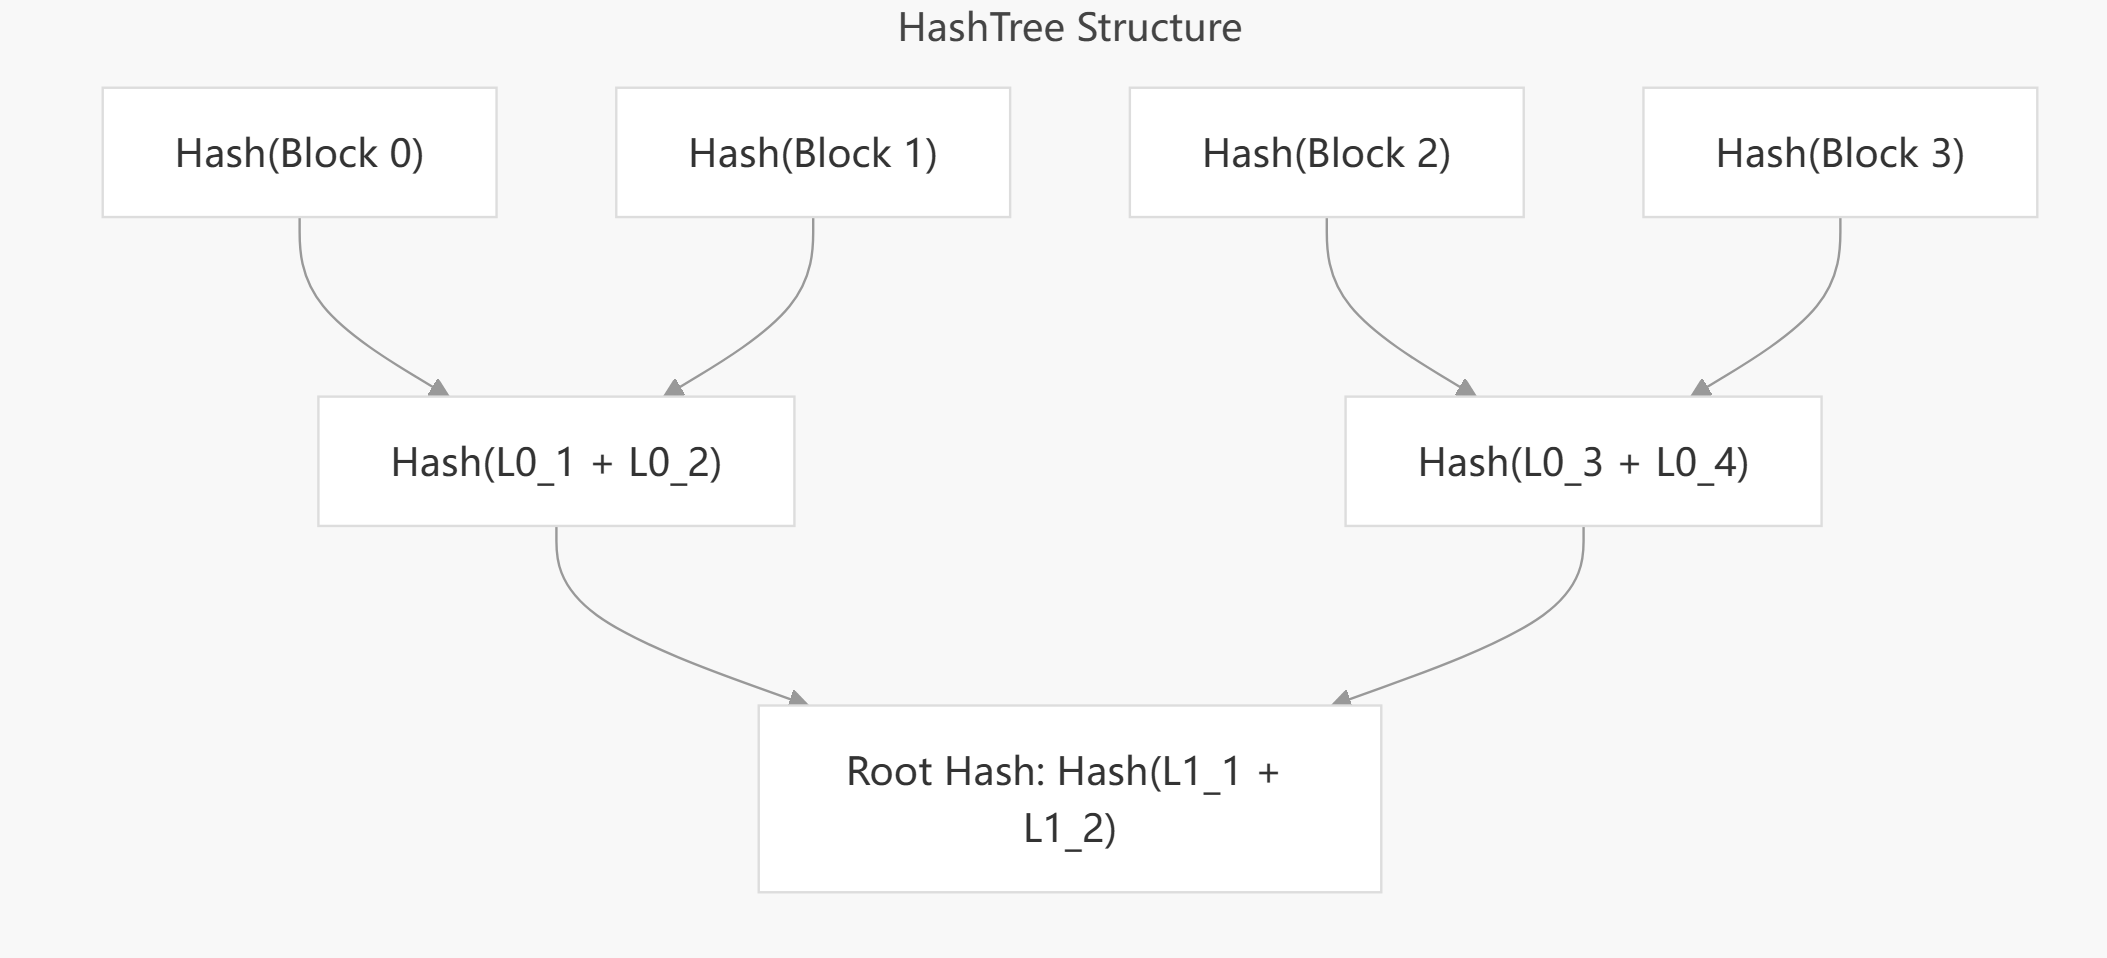
\includegraphics[width=0.9\textwidth]{merkle_tree_flow.png}
    \caption{默克尔树构建与校验数据流图}
    \label{fig:merkle_tree}
\end{figure}

\subsection{BlockDevice 抽象与可组合映射器链调研}

本项目调研并借鉴了星绽操作系统的 \texttt{BlockDevice} trait 设计，该 trait 是所有块 I/O 操作的基础接口：

\begin{lstlisting}[language=Rust, basicstyle=\ttfamily\small, breaklines=true]
pub trait BlockDevice: Send + Sync {
    fn block_size(&self) -> usize;
    fn num_blocks(&self) -> u64;
    fn read_block(&self, block_id: u64, buf: &mut [u8]) -> Result<()>;
    fn write_block(&self, block_id: u64, buf: &[u8]) -> Result<()>;
}
\end{lstlisting}

所有 I/O 方法均返回 \texttt{Result<()>}，其中错误被封装在 \texttt{DmError} 枚举中。该 trait 要求实现 \texttt{Send} 和 \texttt{Sync}，使得所有后端均可安全地跨线程共享。

基于此抽象，本项目采用类似装饰器（Decorator）的设计模式：映射器（如 \texttt{DmCryptDevice} 和 \texttt{DmVerityDevice}）既实现了 \texttt{BlockDevice} trait，又在内部包装另一个实现了 \texttt{BlockDevice} 的对象，从而支持功能的任意堆叠与组合。例如，典型的栈可以是 \texttt{FileBlockDevice $\to$ DmCryptDevice $\to$ DmVerityDevice}。

\begin{figure}[H]
    \centering
    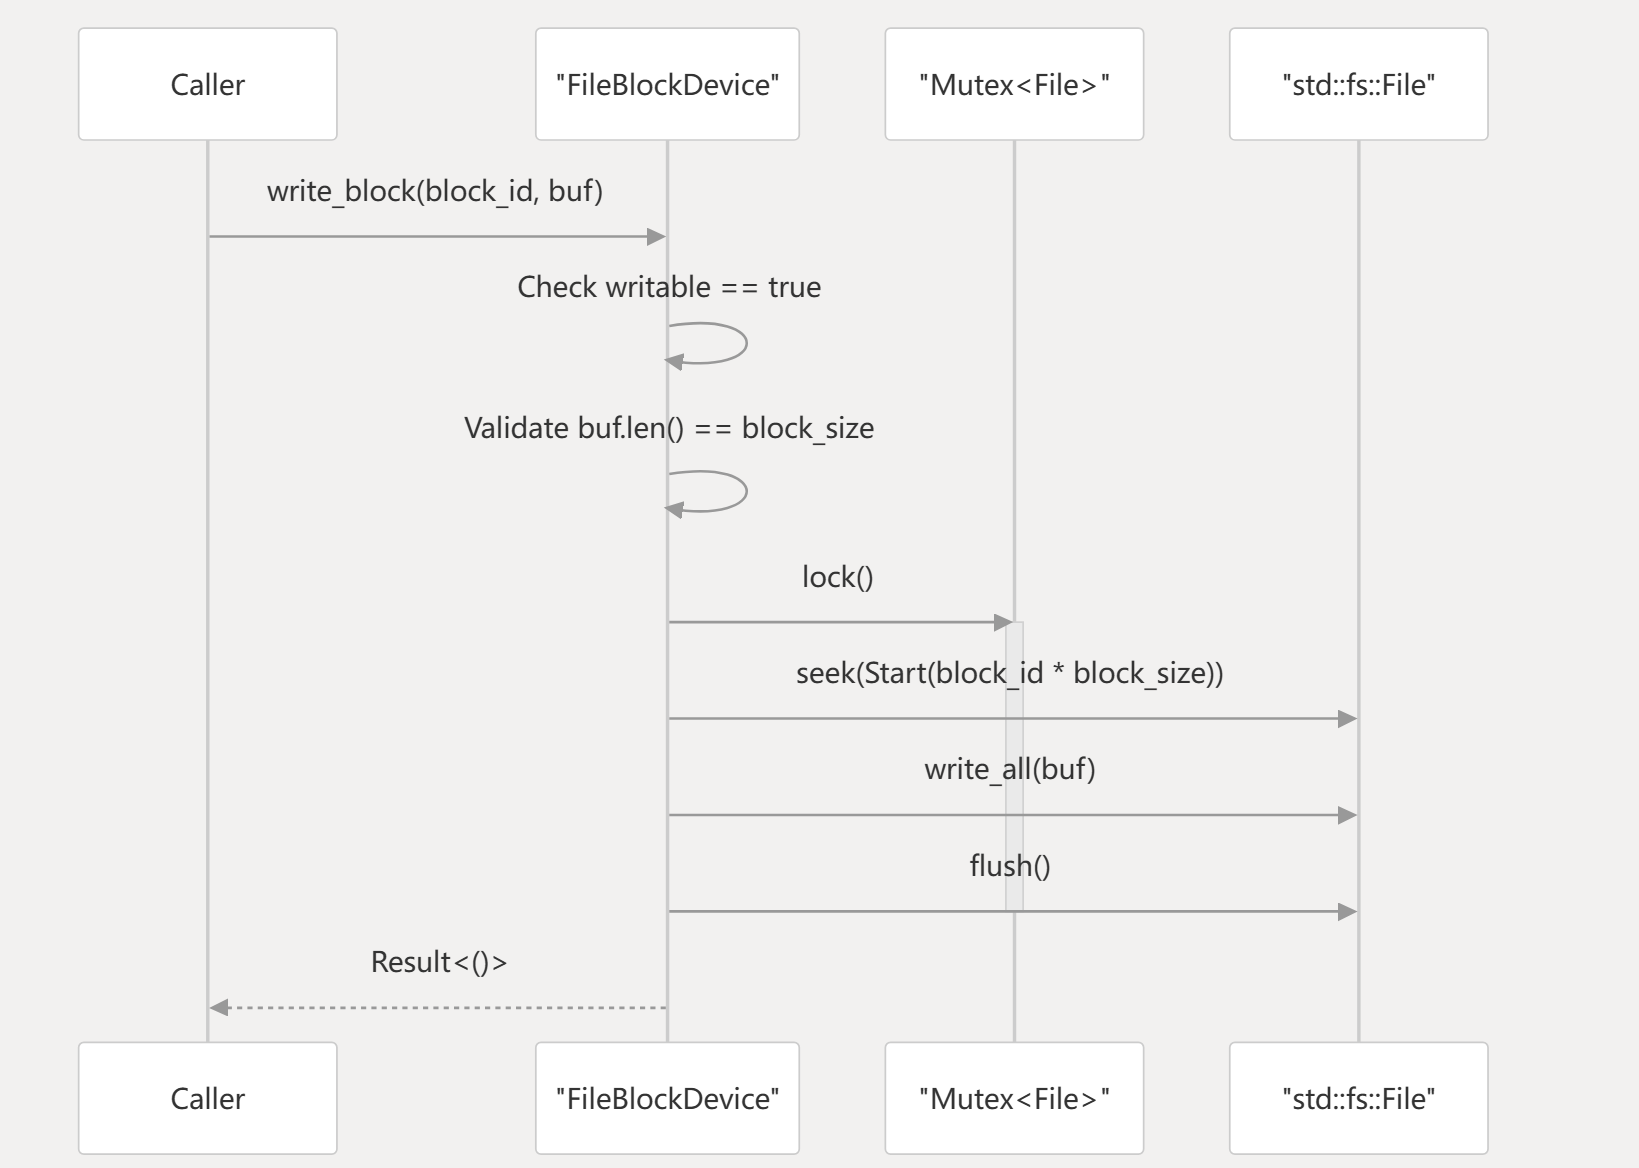
\includegraphics[width=0.9\textwidth]{blockdevice_trait_uml.png}
    \caption{BlockDevice Trait 与后端实现关系图}
    \label{fig:blockdevice_trait}
\end{figure}

该抽象已在用户态（\texttt{dmctl} 使用 \texttt{FileBlockDevice}）和星绽内核（\texttt{aster-dm} 使用 \texttt{VirtioBlkAdapter}）中得到统一实现，验证了跨环境可移植性的可行性。

\subsection{Rust 在可信存储领域的独特优势}

选择 Rust 而非 C 实现可信存储模块，具有以下独特优势：

\begin{enumerate}
    \item \textbf{内存安全}：Rust 的所有权和借用检查在编译期杜绝了悬垂指针、use-after-free 和缓冲区溢出——这些正是 C 内核中安全漏洞的主要来源（据统计约占 Linux 内核漏洞的 65\%）。在可信存储场景中，内存安全漏洞可能导致密钥泄露或完整性绕过。
    
    \item \textbf{类型系统编码安全属性}：Rust 的类型系统可以将安全属性编码到类型中。例如，本项目中的 \texttt{TargetCapabilities} 结构体使组合栈的安全能力（confidentiality、integrity、read\_only）可在编译期静态检查。
    
    \item \textbf{零成本抽象}：Rust 的 trait 和泛型不会引入运行时开销，使得抽象（如 \texttt{BlockDevice}）可以像手写 C 代码一样高效，同时保持代码可复用性。
    
    \item \texttt{Send} 和 \texttt{Sync} 的自动推导：Rust 通过这两个标记 trait 在编译期保证线程安全，避免了 C 内核中因锁使用不当导致的竞态条件。
    
    \item \textbf{更安全的错误处理}：\texttt{Result<T, E>} 强制开发者显式处理错误，避免了 C 内核中因错误码被忽略而导致的静默失败。
\end{enumerate}

本项目正是 Rust 在可信存储领域优势的实践验证——我们使用相同的核心算法（AES-XTS、SHA-256）实现了与 Linux 兼容的可信存储，同时获得了 Rust 提供的安全保障。

\subsection{参考实现与开源生态调研}

\begin{table}[H]
    \centering
    \begin{tabular}{p{0.20\textwidth}p{0.32\textwidth}p{0.38\textwidth}}
        \toprule
        \textbf{名称} & \textbf{来源/位置} & \textbf{参考内容与启示} \\
        \midrule
        Linux 内核 dm-crypt & \texttt{\seqsplit{drivers/md/dm-crypt.c}} & XTS 实现细节、plain64 IV 生成、table 格式解析 \\
        Linux 内核 dm-verity & \texttt{\seqsplit{drivers/md/dm-verity.c}} & Merkle 树 on-disk 布局、验证逻辑、缓存策略 \\
        cryptsetup 工具 & \texttt{\seqsplit{https://gitlab.com/cryptsetup/cryptsetup}} & 用户态控制协议、LUKS 格式、plain 模式 open/close \\
        RustCrypto \texttt{aes} & \texttt{\seqsplit{https://crates.io/crates/aes}} & AES 算法接口设计参考（本项目为独立实现） \\
        RustCrypto \texttt{xts-mode} & \texttt{\seqsplit{https://crates.io/crates/xts-mode}} & XTS 模式 API 参考（本项目为独立实现） \\
        NIST SP 800-38E & \texttt{\seqsplit{nvlpubs.nist.gov/nistpubs/Legacy/SP/}} & XTS-AES 模式标准定义 \\
        FIPS PUB 180-4 & \texttt{\seqsplit{nvlpubs.nist.gov/nistpubs/FIPS/}} & SHA-256 算法标准 \\
        Asterinas 源码 & \texttt{\seqsplit{https://github.com/asterinas/asterinas}} & OSTD 框架、BIO 接口、组件系统 \\
        Asterinas ATC'25 论文 & USENIX ATC 2025 & Framekernel 架构、TCB 最小化设计理念 \\
        《The Rust Programming Language》 & \texttt{\seqsplit{https://doc.rust-lang.org/book/}} & Rust 系统编程、\texttt{no\_std} 开发 \\
        \bottomrule
    \end{tabular}
\end{table}

\subsection{兼容性验证策略调研}

为确保与 Linux 生态的互操作性，本项目设计了分层兼容性验证策略：

\begin{enumerate}
    \item \textbf{算法层}：固定向量测试——AES-XTS 已知明文测试向量、SHA-256 标准测试向量（空字符串、\texttt{"abc"}）；
    \item \textbf{协议层}：与 Linux 内核 dm-crypt 逐字节比对——同一密钥（512 位）、同一明文（0x5a 填充的一个扇区）、同一扇区号（扇区 0）生成的密文 SHA-256 一致；
    \item \textbf{工具层}：在 Asterinas KVM 中运行标准 \texttt{cryptsetup} 工具（plain 模式），验证 \texttt{open}、\texttt{dd read}、\texttt{close} 完整流程（R01）；
    \item \textbf{性能层}：使用与 Linux 相同的 fio 参数和 workload，在同一 backing image 上分别测试，确保可比性；
    \item \textbf{正确性层}：通过物理篡改（单字节翻转）验证 dm-verity 的检测能力，确保完整性边界未被削弱（V03--V07）。
\end{enumerate}

\section{技术可行性评估}

基于上述调研，本项目从以下维度评估技术可行性：

\begin{table}[H]
    \centering
    \begin{tabular}{p{0.20\textwidth}p{0.35\textwidth}p{0.35\textwidth}}
        \toprule
        \textbf{维度} & \textbf{风险评估} & \textbf{应对措施} \\
        \midrule
        算法正确性 & \textbf{低风险}：AES-XTS 和 SHA-256 有明确标准和参考实现 & 固定向量测试 + Linux 逐字节比对 \\
        Linux 兼容性 & \textbf{中风险}：plain64 IV 和 XTS 实现细节易出错 & 早期编写交叉验证脚本，迭代修正 \\
        Asterinas 集成 & \textbf{中风险}：BIO 接口和启动流程需要深入理解 & 补丁序列渐进式集成，每步独立验证 \\
        性能达标 & \textbf{中风险}：虚拟机环境 I/O 性能波动大 & 固定五轮、交替顺序、保留原始数据 \\
        优化不削弱安全 & \textbf{高风险}：缓存可能绕过完整性校验 & “先认证后插入”设计原则 + 计数器验证 \\
        \bottomrule
    \end{tabular}
\end{table}

项目的总体可行性判断为\textbf{高可行}，理由如下：

\begin{enumerate}
    \item 核心算法有明确的标准（NIST、FIPS）和参考实现（Linux 内核），验证手段成熟；
    \item 双目标架构（用户态 + 内核态）使用户态可作为“安全网”，在进入内核前充分验证算法和逻辑；
    \item Asterinas 提供了清晰的组件接入接口（\texttt{Components.toml}、\texttt{aster-cmdline}、\texttt{aster-block}），集成路径明确；
    \item 性能测试合同（\texttt{benchmark\_contract.md}）固定了环境、参数、轮数和统计口径，结果可复现、可审计。
\end{enumerate}

\section{小结}

本章从赛题要求、赛题特征、技术挑战、课程关联、相关技术调研（含 Linux Device Mapper、星绽架构、AES-XTS、SHA-256、默克尔树、\texttt{BlockDevice} 抽象、Rust 优势）、参考实现和兼容性验证策略十个维度对比赛题目进行了全面分析。

核心调研结论包括：
\begin{enumerate}
    \item Linux Device Mapper 框架提供了成熟的 dm-crypt/dm-verity 参考实现，但 Asterinas 的内核接口与之不同，需要从头实现 Rust 适配层；
    \item AES-256-XTS 和 SHA-256 有明确的标准规范，通过固定向量和 Linux 逐字节比对可验证兼容性；默克尔树的 on-disk 布局设计使得标准 ext2 镜像可与哈希树共存；
    \item Rust 的所有权系统、类型系统和零成本抽象为可信存储模块提供了 C 语言无法比拟的内存安全和可组合性；\texttt{BlockDevice} trait 的统一抽象为跨环境可移植性奠定了基础；
    \item 双目标架构（用户态验证 + 内核态集成）和分层兼容性验证策略确保了项目的可验证性和可复现性；
    \item 赛题要求的 QEMU + virtio-blk 标准化测试环境已在本项目中完整实现并用于所有验证。
\end{enumerate}

基于统一抽象、渐进式集成和可观测性内置的技术路线，项目具备充分的可行性和可验证性。后续章节将详细阐述基于这些分析得出的系统架构设计。

% 第3章：系统框架设计
% chapters/03_framework.tex
\chapter{系统框架设计}

\section*{本章框架设计速览}

\begin{table}[H]
    \centering
    \begin{tabular}{p{0.18\textwidth}p{0.35\textwidth}p{0.37\textwidth}}
        \toprule
        \textbf{设计维度} & \textbf{核心决策} & \textbf{技术收益} \\
        \midrule
        核心抽象 & \texttt{BlockDevice} trait & 后端与 mapper 可互换、可堆叠 \\
        架构模式 & 装饰器 + 组合 & \texttt{Passthrough $\to$ Crypt $\to$ Verity} \\
        双目标 & 核心逻辑与平台无关 & 用户态验算法，内核态走真 BIO \\
        同步 & 用户态 \texttt{Mutex}；内核 \texttt{spin::Mutex} + 关抢占 & AES-NI 期间 XMM 不被打断 \\
        能力传播 & \texttt{TargetCapabilities} & 组合栈机密性/完整性/只读可静态汇总 \\
        可观测 & 原子计数器 + 阶段计时 & \texttt{/proc/dm-*-stats} 归因 \\
        \bottomrule
    \end{tabular}
\end{table}

\section{设计原则}

本项目的基本设计原则是使用统一的抽象来表示任何能够进行块级 I/O 的实体，并采用"分层"或"可组合"的架构，使加密和校验逻辑与底层存储介质完全解耦。核心设计原则包括：

\begin{enumerate}
    \item \textbf{统一抽象}：所有存储后端和映射器均实现同一个 \texttt{BlockDevice} trait，确保模块可互换、可堆叠；
    \item \textbf{双目标共享}：核心逻辑与平台无关，同时服务于用户态命令行工具（\texttt{dmctl}）和星绽内核（\texttt{aster-dm}）；
    \item \textbf{安全优先}：所有优化（缓存、缓冲池）遵循"先认证后使用"原则，不削弱安全边界；
    \item \textbf{可观测性内置}：关键路径嵌入原子计数器和阶段计时，支持性能归因和优化验证。
\end{enumerate}

这些原则共同确保了系统的可扩展性、可验证性和安全性——这正是 Device Mapper 作为可信存储底座的核心质量要求。

\section{核心抽象：BlockDevice Trait}

\texttt{BlockDevice} trait 是库中所有存储操作的基础接口，定义了用于读写固定大小数据块的同步接口。为了支持跨线程的并发访问并安全地集成到星绽内核或用户态工具中，该 trait 要求实现 \texttt{Send} 和 \texttt{Sync} 标记。Rust 通过这两个标记 trait 在编译期自动推导类型是否可安全地跨线程共享，无需开发者手动判断。

该 trait 定义如下：

\begin{lstlisting}[language=Rust, basicstyle=\ttfamily\small, breaklines=true]
pub trait BlockDevice: Send + Sync {
    fn block_size(&self) -> usize;
    fn num_blocks(&self) -> u64;
    fn read_block(&self, block_id: u64, buf: &mut [u8]) -> Result<()>;
    fn write_block(&self, block_id: u64, buf: &[u8]) -> Result<()>;
}
\end{lstlisting}

所有 I/O 方法均返回 \texttt{Result<()>}，其中错误被封装在 \texttt{DmError} 枚举中，涵盖无效块大小、无效块号、密钥错误、完整性违规等场景。这个 trait 的设计借鉴了 Linux 内核 \texttt{block\_device\_operations} 的职责分离思想，但通过 Rust 的类型系统提供了更强的安全性保证——任何不安全的跨线程访问在编译期就会被阻止。

在 Asterinas 内核中，该 trait 进一步映射到 \texttt{aster-block} 组件的 BIO 接口，从而支持真实的 VirtIO 块设备。

\section{可组合的映射器链模式}

该架构采用类似装饰器（Decorator）的设计模式。每个映射器（如 \texttt{DmCryptDevice} 和 \texttt{DmVerityDevice}）既实现了 \texttt{BlockDevice} trait，又在内部消费（包装）另一个实现了 \texttt{BlockDevice} 的对象，支持功能的任意堆叠与组合。

例如，一个典型的用户态栈可能是：

\begin{lstlisting}[language=Rust, basicstyle=\ttfamily\small, breaklines=true]
let file = FileBlockDevice::open("disk.img")?;
let crypt = DmCryptDevice::new(file, key)?;
let verity = DmVerityDevice::open(crypt, tree, root_hash)?;
\end{lstlisting}

在星绽内核中，这种组合通过 \texttt{DmDevice} 结构体实现，它根据 \texttt{DmTarget} 枚举（Passthrough、Crypt、Verity）分发 BIO 请求。由于每个 mapper 的下层是 \texttt{Arc<dyn BlockDevice>}，启动阶段可将 \texttt{rootfs\_verity.device} 指向已注册的 crypt mapper 名（如 \texttt{dm-crypt0}），或显式设置 \texttt{dm\_stack=crypt,verity}，从而形成与用户态相同的叠栈：\texttt{vdc $\to$ dm-crypt0 $\to$ dm-verity0}。验收脚本为 \texttt{scripts/run\_dm\_stack.sh}。

\section{核心模块分解}

项目被结构化为离散的模块，以清晰地分离密码学原语、数据结构和设备逻辑。整个 \texttt{dm} crate 约 3000 行 Rust 代码，\texttt{dmctl} 约 800 行；内核补丁 0001--0007 约 4000 行。不是两套互不相干的实现：用户态是算法与布局的安全网，内核态才是赛题交付物。模块划分如下：

\begin{table}[H]
    \centering
    \caption{核心模块职责划分与代码量}
    \begin{tabular}{p{0.16\textwidth}p{0.38\textwidth}p{0.10\textwidth}p{0.26\textwidth}}
        \toprule
        \textbf{模块} & \textbf{主要职责} & \textbf{约行数} & \textbf{关键实体} \\
        \midrule
        \texttt{block\_device} & 抽象与文件/内存后端 & 400 & \texttt{BlockDevice}, \texttt{FileBlockDevice}, \texttt{MemoryBlockDevice} \\
        \texttt{dm\_crypt} & AES-XTS 透明加密 & 350 & \texttt{DmCryptDevice}, \texttt{DmCryptTable} \\
        \texttt{dm\_verity} & 只读完整性 & 200 & \texttt{DmVerityDevice} \\
        \texttt{hash\_tree} & Merkle 构建与校验 & 150 & \texttt{HashTree} \\
        \texttt{sha256} & 纯 Rust SHA-256 & 120 & \texttt{sha256::sha256} \\
        \texttt{device\_mapper} & 链接与 \texttt{DmStackBuilder} & 180 & \texttt{PassthroughDevice}, \texttt{DmStackBuilder} \\
        \texttt{statistics} & I/O 与阶段归因 & 150 & \texttt{InstrumentedDevice}, \texttt{IoStatsSnapshot} \\
        \texttt{runtime} & 运行时 mapper / \texttt{dm\_ioctl} & 260 & \texttt{RuntimeMapper}, \texttt{DmControlDevice} \\
        \bottomrule
    \end{tabular}
\end{table}

\texttt{BlockDevice} 实现涵盖了多种后端场景：
\begin{itemize}
    \item \texttt{MemoryBlockDevice}：基于内存向量的设备，主要用于单元测试和易失性存储；
    \item \texttt{FileBlockDevice}：由宿主机文件系统上的文件支持的持久化设备，由 \texttt{dmctl} 工具使用；
    \item \texttt{PassthroughDevice}：将调用直接转发给内部设备的包装器，用于验证映射器链；
    \item \texttt{VirtioBlkAdapter}：（星绽移植版）将内核特定的块设备句柄适配到 \texttt{BlockDevice} 接口，位于 \texttt{aster-dm} 组件中。
\end{itemize}

\section{双目标架构：跨环境可移植性}

一个核心设计目标是：相同的逻辑同时服务于用户态演示和星绽内核。这是通过严格隔离环境特定代码来实现的。

\begin{figure}[H]
    \centering
    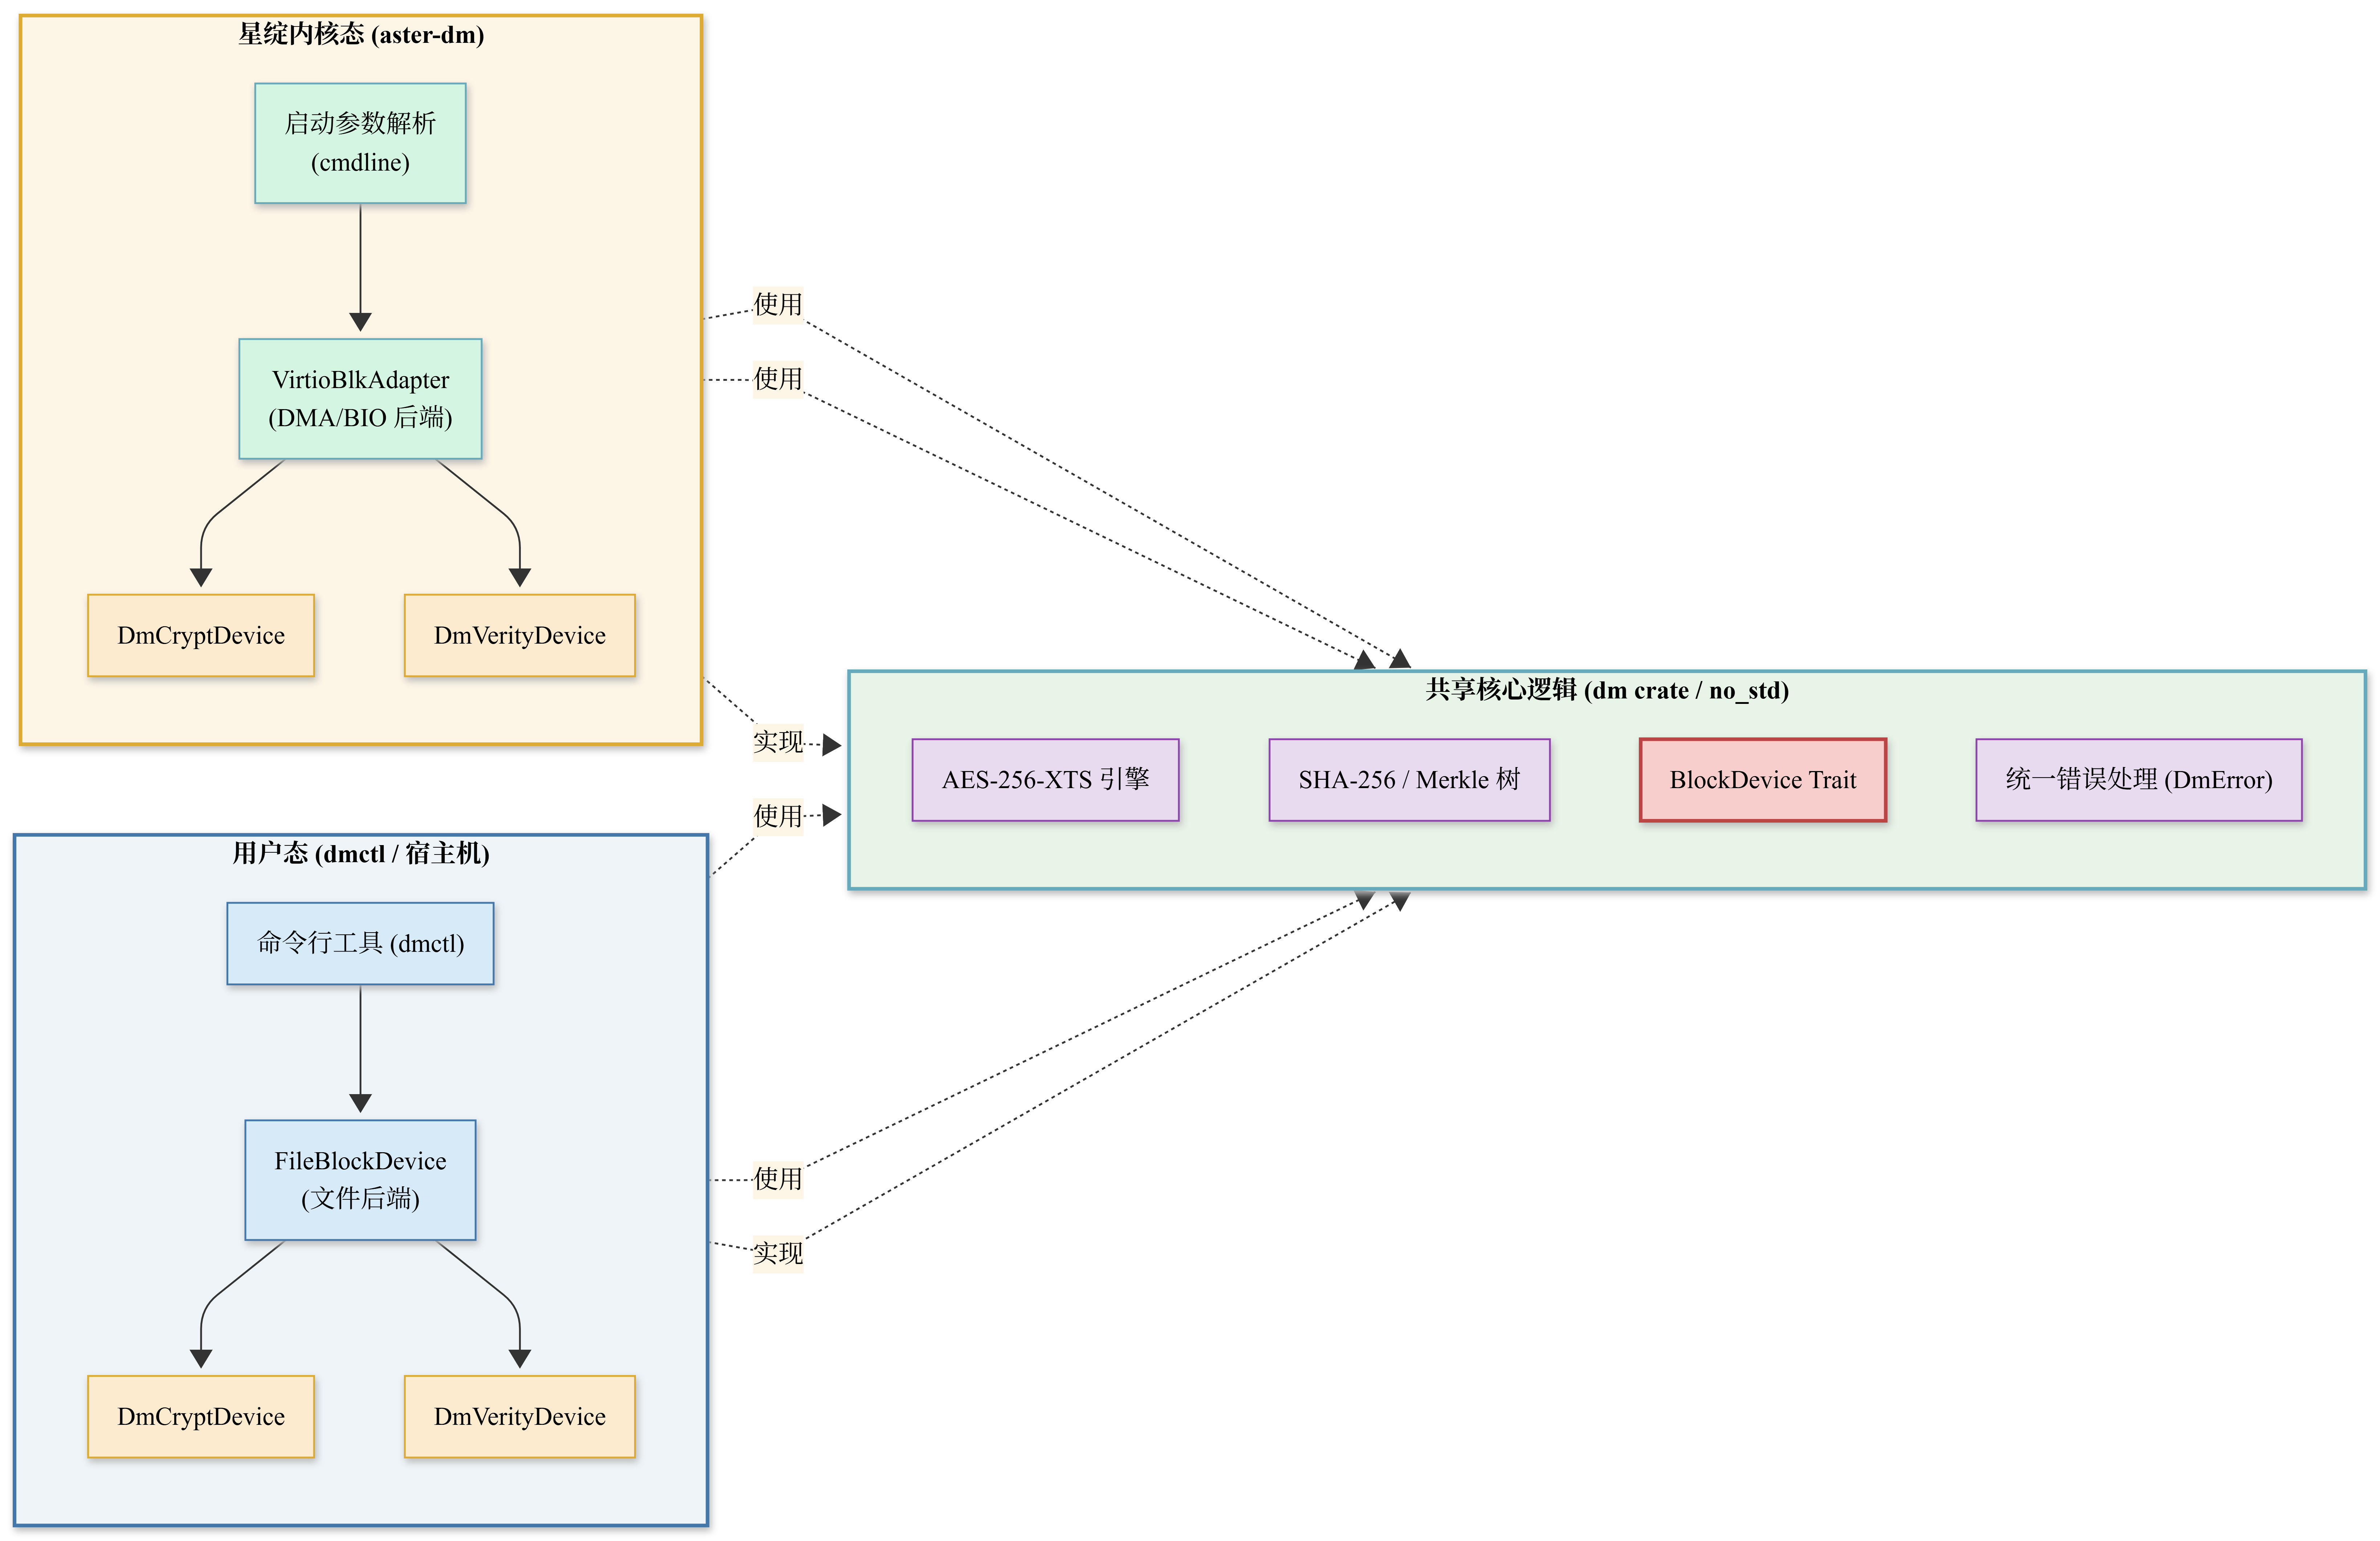
\includegraphics[width=0.95\textwidth]{code_entity_mapping_userspace_kernel.png}
    \caption{代码实体映射图（用户态 vs 星绽内核）}
    \label{fig:code_entity_mapping}
\end{figure}

如上图所示，用户态和内核态共享同一套核心算法实现（AES-XTS、SHA-256、Merkle 树验证），但适配层完全隔离：

\begin{itemize}
    \item \textbf{用户态}：\texttt{dmctl} 工具实例化一个 \texttt{FileBlockDevice}，并根据命令行参数将其包装在 \texttt{DmCryptDevice} 或 \texttt{DmVerityDevice} 中；所有 I/O 操作是同步的，使用 \texttt{std::sync::Mutex} 保证线程安全。
    \item \textbf{内核态}：在星绽中，\texttt{VirtioBlkAdapter} 包装了内核内部的块设备句柄。由于该适配器实现了 \texttt{BlockDevice}，\texttt{DmCryptDevice} 可以无需任何修改地直接包装它；I/O 操作是异步的（BIO），使用 \texttt{spin::Mutex} 和原子操作保证并发安全，在 AES-NI 变换期间还须通过 \texttt{disable\_preempt} 和 \texttt{irq::disable\_local} 保护 XMM 寄存器。
    \item \texttt{no\_std} 兼容性：核心 \texttt{dm} 库设计为最小化依赖（例如，\texttt{aes} crate 设置 \texttt{default-features = false}），以促进在可能限制标准库的内核环境中执行。
\end{itemize}

代码实体映射关系如下：

\begin{table}[H]
    \centering
    \caption{用户态与内核态实体映射}
    \begin{tabular}{p{0.22\textwidth}p{0.33\textwidth}p{0.35\textwidth}}
        \toprule
        \textbf{功能} & \textbf{用户态（dmctl）} & \textbf{内核态（aster-dm）} \\
        \midrule
        代码 & \texttt{crates/dm/}、\texttt{crates/dmctl/} & \texttt{asterinas/kernel/comps/dm/}，补丁 \texttt{asterinas\_port/patches/} 0001--0007 \\
        块设备后端 & \texttt{FileBlockDevice} / \texttt{MemoryBlockDevice} & \texttt{VirtioBlkAdapter}（virtio-blk BIO） \\
        加密映射器 & \texttt{DmCryptDevice} & \texttt{DmTarget::Crypt} \\
        完整性映射器 & \texttt{DmVerityDevice} & \texttt{DmTarget::Verity} \\
        组合构建器 & \texttt{DmStackBuilder} / \texttt{demo-stack} & \texttt{dm\_stack=crypt,verity}（补丁 0007） \\
        控制接口 & 命令行、\texttt{crypt-table-fill} & \texttt{/dev/mapper/control}（供 cryptsetup） \\
        同步 & \texttt{std::sync::Mutex} & \texttt{spin::Mutex} + \texttt{disable\_preempt} \\
        \bottomrule
    \end{tabular}
\end{table}

\section{数据流架构}

下图展示了应用程序的 I/O 请求如何穿过该分层栈：

\begin{figure}[H]
    \centering
    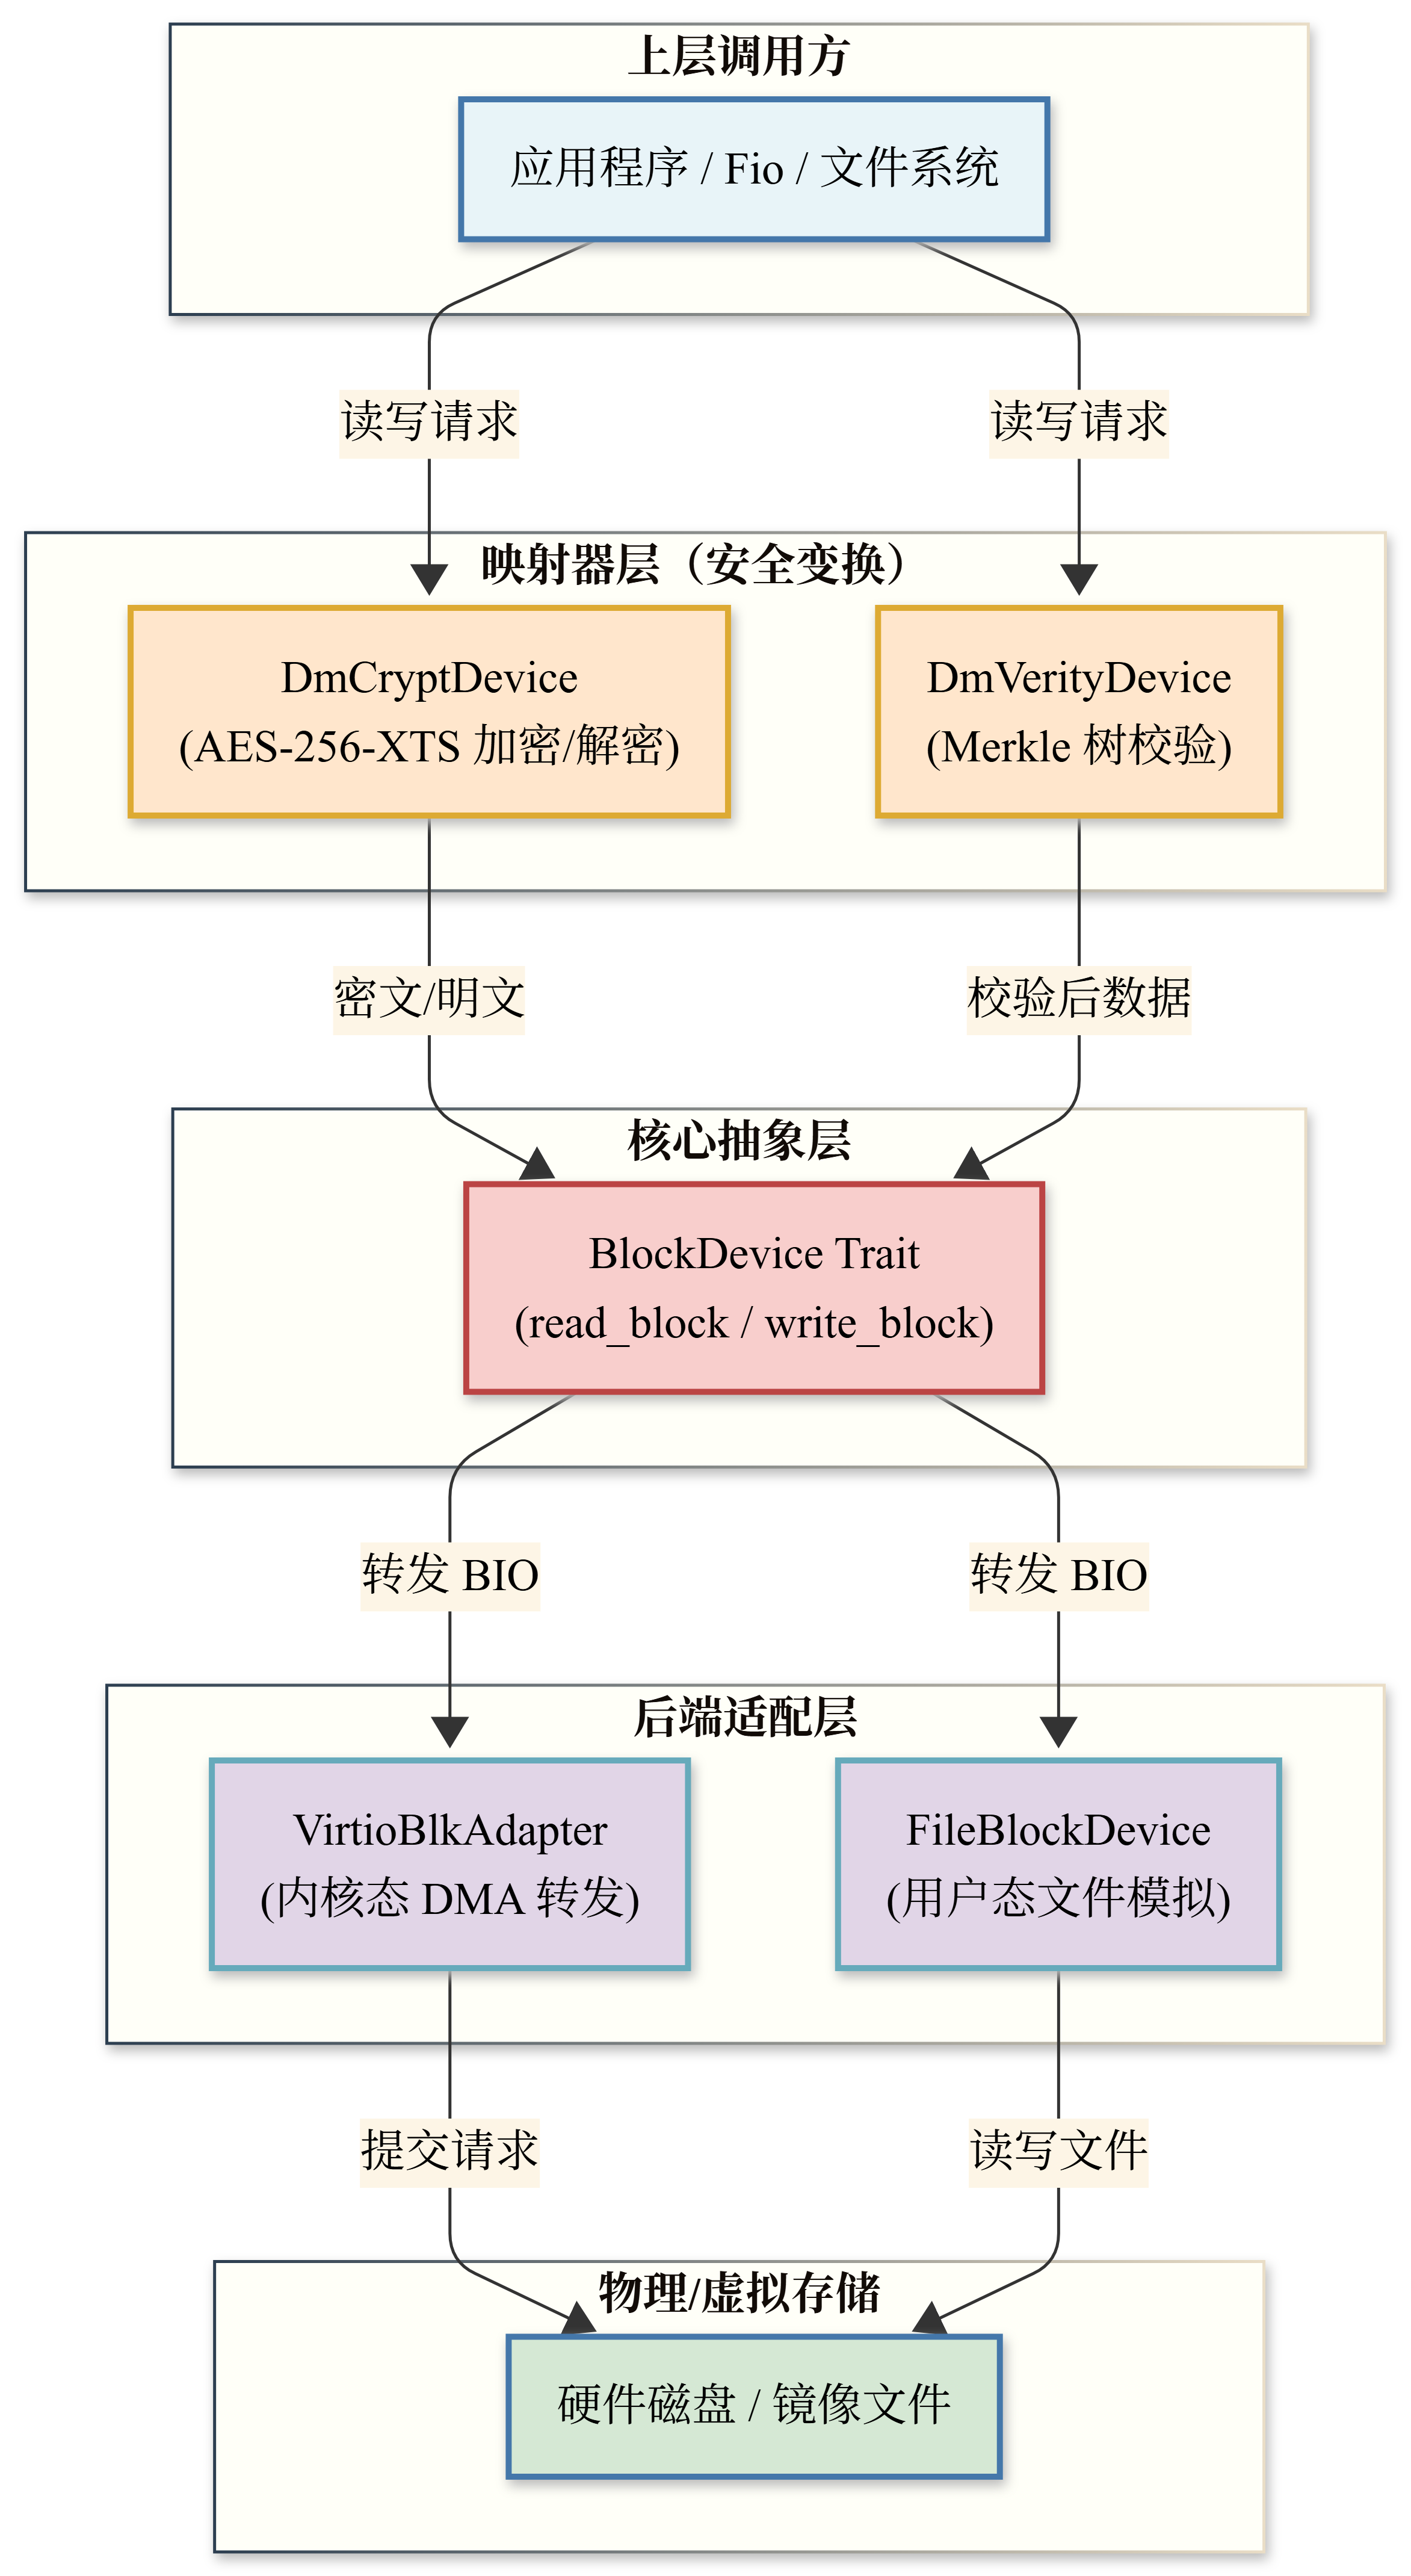
\includegraphics[width=0.9\textwidth]{block_io_layered_stack.png}
    \caption{块 I/O 分层栈数据流图}
    \label{fig:io_stack}
\end{figure}

在此模型中，\texttt{DmCryptDevice} 在执行 AES-256-XTS 转换后，将生成的密文传递给链中的下一个设备。类似地，\texttt{DmVerityDevice} 拦截读请求，以根据 Merkle 树校验数据的完整性。

\subsection{dm-crypt 数据流}

\textbf{写入路径}：按块号算扇区 $\to$ scratch 缓冲 $\to$ AES-XTS（扇区号作 plain64 IV）$\to$ 下层设备。4 KiB 块拆成 8 个 512 字节扇区分别变换，才能和 Linux 一致。具体步骤：

\begin{enumerate}
    \item 应用程序或文件系统向 \texttt{DmCryptDevice} 发起 \texttt{write\_block} 请求；
    \item 根据逻辑块 ID 和 \texttt{iv\_offset} 计算对应的物理扇区号；
    \item 从 scratch pool 获取临时缓冲区，调用 \texttt{Aes256XtsCipher} 对数据进行加密，使用扇区号作为 plain64 IV；
    \item 通过 \texttt{BioSegment::alloc\_bytes} 创建 bounce segment，将密文写入底层 \texttt{BlockDevice}；
    \item 底层设备完成写入后，释放 scratch 缓冲区，完成上层 BIO。
\end{enumerate}

\textbf{读取路径}是上述过程的逆操作：从底层设备读取密文到 scratch 缓冲区，使用相同的扇区号进行解密，然后写回上层 segment，最后释放 scratch 缓冲区。

\subsection{dm-verity 数据流}

\textbf{读取路径}：读数据块 $\to$ SHA-256 $\to$ 沿 on-disk 树或认证后缓存走到 root hash $\to$ 不一致则 \texttt{IntegrityViolation}。\textbf{写一律拒绝}。具体步骤：

\begin{enumerate}
    \item 从底层块设备读取原始数据块；
    \item \texttt{HashTree::verify\_block} 计算检索到的数据的 SHA-256 哈希值；
    \item 在每一层，从 on-disk 哈希树或认证后缓存中检索对应哈希值；
    \item 将重新计算出的哈希值与 \texttt{DmVerityDevice} 中存储的 root hash 进行比对；
    \item 如果哈希值不匹配，返回 \texttt{IntegrityViolation} 错误；若匹配且哈希块此前未缓存，则将其插入认证后缓存供后续复用。
\end{enumerate}

\section{线程安全保证}

所有后端均实现了 \texttt{Sync}，允许跨线程共享：

\begin{itemize}
    \item \texttt{MemoryBlockDevice}：在整个块向量周围使用 \texttt{Mutex}，确保安全性但将所有 I/O 串行化；
    \item \texttt{FileBlockDevice}：在 \texttt{File} 对象周围使用 \texttt{Mutex}，锁在 seek、read/write 和 flush 序列的整个持续时间内被持有；
    \item \texttt{PassthroughDevice}：依赖于底层设备实现了 \texttt{Sync}。
\end{itemize}

在星绽内核中，\texttt{DmDevice} 通过 \texttt{enqueue} 方法处理 BIO，内部使用 \texttt{spin::Mutex} 保护共享状态（如 \texttt{CryptScratchPool} 和 \texttt{VerifiedHashBlockCache}），并遵循内核的并发模型。内核态使用自旋锁而非睡眠锁的原因是——在 BIO 完成回调等中断上下文中不能睡眠，而自旋锁可以在禁用抢占和中断的情况下安全地持有，不会导致调度延迟或死锁。AES-NI 变换期间通过 \texttt{disable\_preempt} 和 \texttt{irq::disable\_local} 确保 XMM 寄存器不被中断上下文破坏——这是因为 AES-NI 指令使用 XMM 寄存器，而中断处理程序可能复用这些寄存器导致数据损坏。

\section{性能可观测性设计}

为了支持性能归因和优化验证，架构中集成了统计模块：

\begin{itemize}
    \item \texttt{InstrumentedDevice}：一个装饰器，可以插入到任意两层之间，记录读/写次数、字节数、失败次数以及累计和最大延迟（以纳秒计）；
    \item \texttt{IoStatsSnapshot}：提供稳定的快照，便于在基准测试前后对比；
    \item 在 Asterinas 内核中，通过启动参数 \texttt{dm.perf\_stats=1} 启用细粒度阶段计时（如 \texttt{lower\_wait}、\texttt{AES-XTS}、\texttt{SHA-256}、\texttt{cache\_lookup} 等），并通过 \texttt{\seqsplit{/proc/dm-performance-stats}} 导出；
    \item \texttt{/proc/dm-verity-stats} 提供 \texttt{verified}、\texttt{bio\_blocks}、\texttt{data\_rereads}、\texttt{hash\_hits}、\texttt{hash\_misses}、\texttt{auth\_shortcuts} 等计数器，直接反映优化效果——这些计数器在正式性能测试中用于验证 BIO 复用（\texttt{data\_rereads=0}）和缓存命中（\texttt{auth\_shortcuts}）的实际收益。
\end{itemize}

内核启用 \texttt{dm.perf\_stats=1} 后的实测归因数据表明：dm-crypt 热路径里下层等待约占 97.84\%、AES-XTS 约占 1.82\%；dm-verity 下层等待约占 93.01\%、数据 SHA-256 约占 5.74\%。算法本身不是主瓶颈，所以优化优先做缓冲池、缓存和 BIO 复用，而不是再改一轮 AES。

这种设计使得开发者可以精确量化每个映射器层的开销，从而指导优化方向。

\section{运行时控制面（Linux 兼容）}

为了支持 \texttt{cryptsetup} 等用户态工具，项目实现了与 Linux \texttt{dm\_ioctl} 兼容的控制接口：

\begin{itemize}
    \item \texttt{DmControlDevice}：在 \texttt{/dev/mapper/control} 提供 ioctl 处理，支持 \texttt{DM\_DEV\_CREATE}、\texttt{DM\_TABLE\_LOAD}、\texttt{DM\_DEV\_SUSPEND}、\texttt{DM\_DEV\_STATUS}、\texttt{DM\_DEV\_REMOVE} 等命令；
    \item \texttt{RuntimeMapper}：管理动态创建的 mapper，包括状态机（Empty、Loaded、Active）和密钥的清除——当 mapper 被删除时，未激活表中的密钥会被显式清零，防止密钥残留在内存中；
    \item 通过该接口，Asterinas 内核可以接受来自 \texttt{cryptsetup} 的标准 table 字符串，动态激活加密映射器，从而实现与 Linux 生态的互操作。
\end{itemize}

\section{安全能力传播}

\texttt{DmStackBuilder} 和 \texttt{DmStack} 提供安全能力的自动汇总：

\begin{lstlisting}[language=Rust, basicstyle=\ttfamily\small, breaklines=true]
pub struct TargetCapabilities {
    pub confidentiality: bool,
    pub integrity: bool,
    pub read_only: bool,
}
\end{lstlisting}

每个 target 声明自己提供的安全能力，最终栈通过 fold 操作自动汇总，使上层调用者可以静态获知组合后的安全属性。例如，\texttt{crypt + verity} 栈自动获得 \texttt{confidentiality=true}、\texttt{integrity=true}、\texttt{read\_only=true}。这种设计将安全策略的传播在编译期完成，避免了运行时动态检查的开销和遗漏风险。

\section{Asterinas 内核集成架构}

\texttt{aster-dm} 组件通过以下方式接入 Asterinas 内核：

\begin{enumerate}
    \item \textbf{组件声明}：在 \texttt{Components.toml} 中注册 \texttt{aster-dm}，在 \texttt{kernel/Cargo.toml} 中引入依赖；
    \item \textbf{启动参数解析}：使用 \texttt{aster-cmdline::define\_kv\_param!} 宏定义 \texttt{dm\_crypt.*}、\texttt{rootfs\_verity.*} 和 \texttt{dm\_stack} 参数；
    \item \textbf{块设备注册}：通过 \texttt{aster\_block::register} 将 mapper 注册为块设备，分配主设备号和次设备号；
    \item \textbf{BIO 处理}：在 \texttt{BlockDevice::enqueue} 中根据 \texttt{DmTarget} 类型分发到对应的处理函数（\texttt{process\_crypt}、\texttt{process\_verity}），所有 I/O 操作均通过 BIO 异步提交；
    \item \textbf{根切换}：initramfs 中的 \texttt{init} 脚本在 \texttt{dm-root} 模式下挂载 mapper，执行 \texttt{pivot\_root} 切换到受保护根。
\end{enumerate}

补丁序列（\texttt{asterinas\_port/patches/0001--0007}）记录了完整的集成演进历史，每一补丁对应一个可独立验证的增量功能，总补丁代码量约 4000 行。补丁用法详见 \texttt{asterinas\_port/README.md}。

\section{小结}

本章详细阐述了系统的核心架构，包括统一的 \texttt{BlockDevice} 抽象、可组合的映射器链模式、模块分解（含约行数）、双目标跨环境可移植性（含代码实体映射表）、数据流架构（含 4 KiB 拆 8 扇区的关键约束和 verity 写拒绝语义）、线程安全保证（含内核/用户态锁策略差异）、性能可观测性设计（含实测归因百分比）、运行时控制面、安全能力传播和 Asterinas 内核集成架构。

关键设计亮点回顾：
\begin{itemize}
    \item \texttt{BlockDevice} trait 作为统一抽象，支撑了整个存储安全框架；
    \item 双目标架构使用户态可作为"安全网"快速验证算法，内核态才是赛题交付物；
    \item Rust 的类型系统（\texttt{Send}、\texttt{Sync}、\texttt{TargetCapabilities}）在编译期保证了线程安全和安全能力传播的正确性；
    \item 性能归因数据表明算法本身不是主瓶颈，优化优先做缓冲池、缓存和 BIO 复用；
    \item 性能可观测性设计将优化决策建立在量化数据之上，而非经验猜测。
\end{itemize}

在接下来的章节中，我们将深入探讨 \texttt{dm-crypt} 和 \texttt{dm-verity} 的具体实现细节，以及如何将上述框架设计落地为可运行的代码。


% 第4章：开发计划
% chapters/04_plan.tex
\chapter{开发计划}

\section*{本章开发计划速览}

\begin{table}[H]
    \centering
    \begin{tabular}{p{0.13\textwidth}p{0.18\textwidth}p{0.28\textwidth}p{0.25\textwidth}}
        \toprule
        \textbf{阶段} & \textbf{时间} & \textbf{核心内容} & \textbf{关键交付物} \\
        \midrule
        第一阶段 & 06-23 -- 06-28 & 用户态核心实现 & \texttt{dm} crate、单元测试、\texttt{dmctl} 工具 \\
        第二阶段 & 06-29 -- 07-10 & Linux 兼容性与工具链 & XTS 兼容验证、\texttt{cryptsetup} plain 模式 \\
        第三阶段 & 07-11 -- 07-20 & 内核补丁与 BIO 集成 & 补丁 0001--0004、rootfs 切换 \\
        第四阶段 & 07-21 -- 07-31 & 性能优化与基准框架 & 补丁 0005--0006、FIO 矩阵脚本 \\
        第五阶段 & 08-01 -- 08-11 & 组合栈与最终验证 & 补丁 0007、五轮性能矩阵、证据归档 \\
        第六阶段 & 08-09 -- 08-18 & 文档整合、答辩与收尾 & 两份 PDF、PPT、视频、最终 README \\
        \bottomrule
    \end{tabular}
\end{table}

\begin{figure}[H]
    \centering
    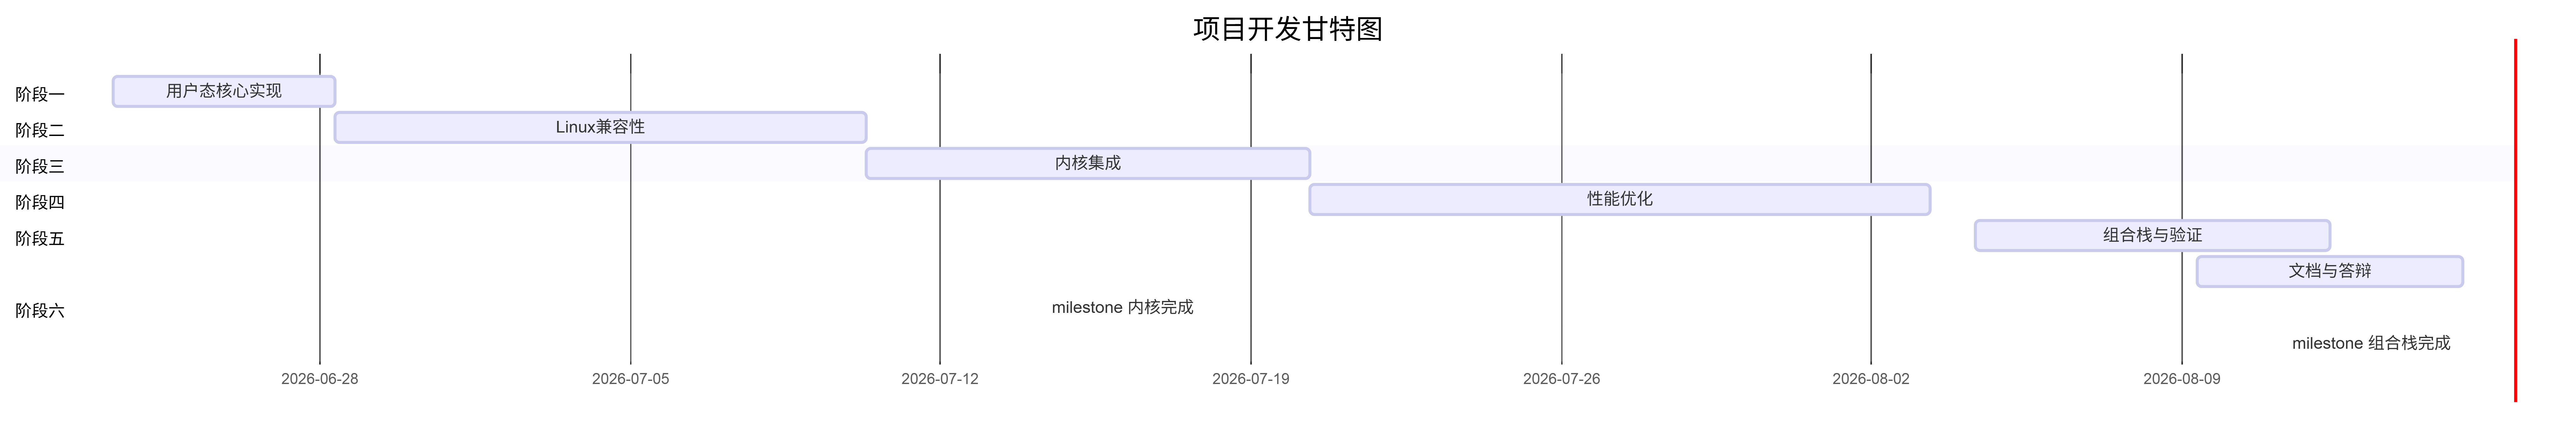
\includegraphics[width=1\textwidth]{development_gantt.png}
    \caption{项目开发甘特图（2026-06-23 至 2026-08-18，全程 57 天）}
    \label{fig:gantt}
\end{figure}

\section{开发方法论}

在制定开发计划时，我们遵循以下方法论原则，确保开发过程可控、可追溯：

\begin{enumerate}
    \item \textbf{先用户态后内核}：所有核心算法（AES-XTS、SHA-256、Merkle 树）先在用户态充分验证，再通过补丁序列接入内核。用户态作为"安全网"，可以在不依赖复杂内核环境的前提下快速迭代和调试；
    \item \textbf{每个补丁一个可验收增量}：补丁 0001：组件骨架与 target；0002：BIO / ext2 魔数自检；0003：\texttt{dm-root} + \texttt{pivot\_root}；0004：\texttt{dm\_ioctl}；0005：性能优化；0006：阶段归因；0007：组合栈。每一步都有明确的验收标准；
    \item \textbf{测完再优化}：正确性 PASS 后再跑正式 FIO；在优化之前先建立性能基准（五轮 FIO、Filebench、SQLite、启动耗时），优化措施的效果通过前后对比量化验证；
    \item \textbf{文档跟代码走}：每个阶段完成后同步更新技术文档和用户手册，避免"代码改完、文档滞后"的常见问题。
\end{enumerate}

上述方法论的核心可概括为\textbf{"先保证安全语义，再接入真实块路径，最后固化复现入口"}。这一原则贯穿了整个开发周期：在用户态用 \texttt{BlockDevice} 抽象验证 AES-XTS、Merkle 树与错误边界；通过 \texttt{VirtioBlkAdapter} 接入 Asterinas BIO，不绕过真实下层设备；分别完成 crypt、verity 与组合栈后，再接入受保护 rootfs；最终使用 Linux 兼容性、KVM 正反例和物理损坏测试作为合入门禁，性能数据必须通过 target、参数和完成语义审计。

\section{阶段划分与时间安排}

本项目实际开发周期为 2026 年 6 月 23 日至 8 月 18 日，共计 57 天，分为六个阶段。其中 08-12 至 08-18 为文档整合与收尾期，完成文档统一、答辩材料提交、表格修订与测试完善。以下按阶段详细描述计划内容与实际完成情况。

\section{第一阶段：用户态核心实现}

\subsection{目标}
在用户态完成 Device Mapper 核心逻辑，不依赖任何操作系统特定接口，使用 \texttt{MemoryBlockDevice} 和 \texttt{FileBlockDevice} 进行验证。这是整个项目的"地基"阶段。

\subsection{任务分解}
\begin{enumerate}
    \item 设计并实现 \texttt{BlockDevice} trait 及内存/文件后端；
    \item 实现 \texttt{sha256} 模块（纯 Rust，无外部依赖，约 120 行）；
    \item 实现 \texttt{hash\_tree} 模块（Merkle 树构建与验证，约 150 行）；
    \item 实现 \texttt{DmCryptDevice}（AES-256-XTS，使用 \texttt{aes} crate，约 350 行）；
    \item 实现 \texttt{DmVerityDevice}（只读完整性校验，约 200 行）；
    \item 实现 \texttt{DmStackBuilder}（可组合映射器链，约 180 行）；
    \item 编写单元测试覆盖核心场景（13+ 个测试）；
    \item 实现 \texttt{dmctl} 命令行工具的基础子命令（约 800 行）。
\end{enumerate}

\subsection{交付物与验收标准}
\begin{itemize}
    \item \textbf{交付物}：\texttt{\seqsplit{crates/dm/src/}} 全部核心模块；\texttt{\seqsplit{crates/dmctl/src/main.rs}} 基础命令
    \item \textbf{验收标准}：
    \begin{enumerate}
        \item \texttt{demo-crypt} 输出 \texttt{ciphertext\_differs: true}；
        \item \texttt{demo-verity} 输出 \texttt{tamper\_detected: true}；
        \item 所有单元测试 PASS。
    \end{enumerate}
\end{itemize}

\subsection{实际完成情况}
\begin{itemize}
    \item 完成时间：2026-06-23（Git commit \texttt{40a52179} \texttt{\seqsplit{feat: add Linux-compatible device mapper implementation}}）；
    \item 通过全部 13+ 个单元测试；
    \item \texttt{demo-crypt} 和 \texttt{demo-verity} 验证通过；
    \item 代码量：约 1500 行 Rust。
\end{itemize}

\section{第二阶段：Linux 兼容性与工具链}

\subsection{目标}
确保 AES-256-XTS 实现与 Linux 内核 \texttt{aes-xts-plain64} 逐字节兼容，并为 \texttt{cryptsetup} 工具提供控制接口。这是确保项目与 Linux 生态互操作的关键阶段。

\subsection{任务分解}
\begin{enumerate}
    \item 实现 \texttt{DmCryptTable} 解析器（支持 Linux table 格式，约 200 行）；
    \item 实现 \texttt{Aes256XtsCipher} 的 \texttt{plain64} IV 语义；
    \item 编写 \texttt{verify\_linux\_xts\_compat.sh} 交叉验证脚本；
    \item 实现 \texttt{/dev/mapper/control} 的 \texttt{dm\_ioctl} 兼容接口（\texttt{dm\_control.rs}，约 520 行）；
    \item 实现 \texttt{RuntimeMapper} 状态机（Empty、Loaded、Active，约 260 行）；
    \item 在 KVM 中验证 \texttt{cryptsetup open/read/close} 流程（R01）。
\end{enumerate}

\subsection{交付物与验收标准}
\begin{itemize}
    \item \textbf{交付物}：\texttt{DmCryptTable} 和 \texttt{\seqsplit{DmCryptDevice::from\_table}}；\texttt{\seqsplit{kernel/src/device/misc/dm\_control.rs}}；\texttt{\seqsplit{kernel/comps/dm/src/runtime.rs}}
    \item \textbf{验收标准}：
    \begin{enumerate}
        \item \texttt{verify\_linux\_xts\_compat.sh} 输出 \texttt{PASS}，SHA-256 匹配；
        \item KVM 中 \texttt{cryptsetup open/read/close} 全部 PASS。
    \end{enumerate}
\end{itemize}

\subsection{实际完成情况}
\begin{itemize}
    \item 完成时间：2026-07-14（补丁 0004）；
    \item Linux XTS 固定向量 SHA-256：\texttt{4334c17f...}；
    \item R01 cryptsetup smoke PASS（证据：\texttt{\seqsplit{R01-cryptsetup-persistent-cache.log}}）；
    \item 代码量：新增约 1000 行内核代码。
\end{itemize}

\section{第三阶段：内核补丁与 BIO 集成}

\subsection{目标}
将 \texttt{aster-dm} 组件完整接入 Asterinas 内核，支持启动参数解析、mapper 注册、BIO 处理和根文件系统切换。这是项目从"用户态玩具"走向"真实内核模块"的关键阶段。

\subsection{任务分解}
\begin{enumerate}
    \item 补丁 0001：组件骨架与 crypt/verity target、VirtIO 适配；
    \item 补丁 0002：BIO 路径与 ext2 魔数自检；
    \item 补丁 0003：\texttt{dm-root} + initramfs 挂载与 \texttt{pivot\_root} 切换；
    \item 补丁 0004：\texttt{dm\_ioctl} 控制面与 mapper 生命周期；
    \item 验证 dm-crypt 根文件系统启动（R02）；
    \item 验证 dm-verity 根文件系统启动（R03/V01）；
    \item 验证单字节篡改拒绝（V02--V07）。
\end{enumerate}

\subsection{交付物与验收标准}
\begin{itemize}
    \item \textbf{交付物}：\texttt{\seqsplit{asterinas\_port/patches/0001--0004.patch}}；\texttt{\seqsplit{tools/run\_dm\_crypt.sh}} 和 \texttt{\seqsplit{tools/run\_dm\_verity.sh}}
    \item \textbf{验收标准}：
    \begin{enumerate}
        \item R02 串口输出 \texttt{PASS system root switched to protected mapper}；
        \item R03/V01 串口输出 \texttt{status=verified} 和根切换 PASS；
        \item V02--V07 篡改后输出 \texttt{status=integrity-rejected}，无根切换 PASS。
    \end{enumerate}
\end{itemize}

\subsection{实际完成情况}
\begin{itemize}
    \item 完成时间：2026-07-14（补丁 0001--0004）；
    \item R01--R03、C01--C05、V01--V07 全部 PASS；
    \item 证据日志位于 \texttt{\seqsplit{docs/evidence/stabilization/correctness-kvm/}}；
    \item 补丁代码量：约 2500 行。
\end{itemize}

\section{第四阶段：性能优化与基准框架}

\subsection{目标}
实现性能优化（AES-NI、scratch pool、hash cache、BIO 复用），并建立可复现的五轮性能基准框架。本阶段的成果直接影响"性能与启动要求"指标的达成。

\subsection{任务分解}
\begin{enumerate}
    \item 补丁 0005：AES-NI 后端、scratch pool、hash cache、正式 benchmark 参数；
    \item 补丁 0006：性能阶段归因（\texttt{/proc/dm-performance-stats}）与正式合同；
    \item 实现 \texttt{scripts/run\_fio\_matrix.sh}（Linux QEMU virtio 与 Asterinas KVM 两平台）；
    \item 实现 Filebench、SQLite、启动耗时测试脚本；
    \item 完成 A/B 对比验证优化效果。
\end{enumerate}

\subsection{交付物与验收标准}
\begin{itemize}
    \item \textbf{交付物}：补丁 0005--0006；\texttt{\seqsplit{scripts/run\_fio\_matrix.sh}}、\texttt{\seqsplit{scripts/run\_filebench\_matrix.sh}}、\texttt{\seqsplit{scripts/run\_sqlite\_matrix.sh}}、\texttt{\seqsplit{scripts/run\_boot\_matrix.sh}}
    \item \textbf{验收标准}：
    \begin{enumerate}
        \item 五轮 FIO 矩阵可自动执行并生成 CSV；
        \item \texttt{dm.perf\_stats=1} 时阶段计时正常输出；
        \item 优化后 \texttt{data\_rereads=0}，\texttt{auth\_shortcuts} > 0。
    \end{enumerate}
\end{itemize}

\subsection{实际完成情况}
\begin{itemize}
    \item 完成时间：2026-08-03（补丁 0005--0006）；
    \item AES-NI 启动日志显示 \texttt{backend=AES-NI}；
    \item 正式性能矩阵于 2026-08-11 完成；
    \item 补丁代码量：约 800 行。
\end{itemize}

\section{第五阶段：组合栈与最终验证}

\subsection{目标}
实现 \texttt{dm-crypt $\to$ dm-verity} 组合栈（补丁 0007），完成全部性能基准测试并归档证据。这是项目从"单层保护"走向"组合保护"的最终形态。

\subsection{任务分解}
\begin{enumerate}
    \item 补丁 0007：\texttt{dm\_stack=crypt,verity} 启动路径；
    \item 实现 \texttt{scripts/build\_stack\_rootfs.sh} 和 \texttt{scripts/run\_dm\_stack.sh}；
    \item 完成 Linux QEMU virtio FIO 13+13 项（raw + dm-crypt）与 verity 读 7 项；
    \item 完成 Asterinas KVM FIO 13+7 项（dm-crypt + dm-verity 读）；
    \item 完成 Filebench、SQLite、启动耗时各 5 轮；
    \item 运行 \texttt{check\_benchmark\_package.py} 验证包完整性。
\end{enumerate}

\subsection{交付物与验收标准}
\begin{itemize}
    \item \textbf{交付物}：补丁 0007；\texttt{\seqsplit{scripts/build\_stack\_rootfs.sh}} 和 \texttt{\seqsplit{scripts/run\_dm\_stack.sh}}
    \item \textbf{验收标准}：
    \begin{enumerate}
        \item 组合栈串口输出 \texttt{stacked mapper: vdc -> dm-crypt0 -> dm-verity0}；
        \item 最终矩阵包含 46 个 PASS 单元格；
        \item \texttt{review\_release\_check.py} 全部通过。
    \end{enumerate}
\end{itemize}

\subsection{实际完成情况}
\begin{itemize}
    \item 完成时间：2026-08-11（补丁 0007，commit \texttt{6385e70b}）；
    \item 最终矩阵 46 PASS + 6 只读 N/A；
    \item 证据目录完整，\texttt{review\_release\_check.py} PASS；
    \item 补丁代码量：约 150 行（组合栈逻辑本身精简，复用已有 crypt/verity 实现）。
\end{itemize}

\section{第六阶段：文档整合、答辩与收尾}

\subsection{目标}
完成两份 PDF（设计赛道文档与技术文档）、答辩 PPT、演示视频的整理与提交，并完成 README 统一、表格修订与测试完善的收尾工作。

\subsection{任务分解}
\begin{enumerate}
    \item 设计赛道文档（\texttt{docs/design\_doc/}，10 章，严格按大赛大纲组织）；
    \item 技术文档（架构设计、模块说明、算法展开、合规与用户手册），两份 PDF 互为补充；
    \item 答辩 PPT（PPTX/PDF）与 8 分钟答辩视频；
    \item 演示视频（含运行环境介绍与受保护 rootfs 启动）；
    \item README 统一为十章策略版，性能表格核对修订；
    \item 测试代码注释完善与全量回归；
    \item AI 工具使用声明。
\end{enumerate}

\subsection{交付物与验收标准}
\begin{itemize}
    \item \textbf{交付物}：\texttt{\seqsplit{docs/design\_doc/design\_doc.pdf}}；技术文档 PDF；答辩 PPT（PPTX/PDF）；8 分钟答辩视频；演示视频；最终 README
    \item \textbf{验收标准}：
    \begin{enumerate}
        \item 所有文档可编译生成 PDF；
        \item 演示视频完整展示受保护 rootfs 启动；
        \item 性能表格与证据目录逐项核对一致；
        \item 全量测试通过；
        \item AI 工具声明完整披露工具名称、模型和使用场景。
    \end{enumerate}
\end{itemize}

\subsection{实际完成情况}
\begin{itemize}
    \item 08-18：两份 PDF、答辩 PPT 与 8 分钟视频定稿，PPT 与视频通过希冀专门入口提交，演示视频上传百度网盘（提取码 \texttt{oscp}）；
    \item 08-16 -- 08-17：README 补全用户态与内核态说明、256 MiB 正式合同与 Linux guest 对照表（\texttt{d56affa8}、\texttt{6e06b136}），技术文档重编并与 README 对齐（\texttt{7cd6d8f1}），设计文档整合（\texttt{9894d4bf}）；
    \item 08-18：FIO 表格修订为 qd=1 配置（\texttt{a0b7aacf}、\texttt{72f6738c}），测试注释完善，最终 README 更新（\texttt{ef345837}），全量测试通过（\texttt{b3247e0e}）。
\end{itemize}

\section{里程碑与关键交付物汇总}

\begin{table}[H]
    \centering
    \caption{关键里程碑与交付物}
    \label{tab:milestones}
    \begin{tabular}{p{0.12\textwidth}p{0.15\textwidth}p{0.55\textwidth}}
        \toprule
        \textbf{里程碑} & \textbf{日期} & \textbf{关键交付物} \\
        \midrule
        M1：用户态核心完成 & 06-23 & \texttt{dm} crate、\texttt{dmctl} 工具、单元测试 PASS（\texttt{40a52179}） \\
        M2：Linux 兼容性验证 & 07-10 & XTS 逐字节兼容证据、\texttt{/dev/mapper/control}（补丁 0004） \\
        M3：内核 rootfs 切换 & 07-14 & R01--R03、C01--C05、V01--V07 全部 PASS（补丁 0001--0004） \\
        M4：性能优化与框架 & 08-03 & AES-NI、scratch pool、hash cache、五轮 FIO 脚本（补丁 0005--0006） \\
        M5：组合栈与最终验证 & 08-11 & 补丁 0007、46 PASS 性能矩阵（\texttt{6385e70b}） \\
        M6：文档答辩定稿 & 08-18 & 两份 PDF、答辩 PPT、视频（希冀专门入口提交） \\
        M7：收尾完成 & 08-18 & README 统一、表格修订、测试全量通过（\texttt{b3247e0e}） \\
        \bottomrule
    \end{tabular}
\end{table}

\section{开发环境与工具链}

\begin{table}[H]
    \centering
    \caption{开发环境依赖}
    \begin{tabular}{p{0.20\textwidth}p{0.25\textwidth}p{0.45\textwidth}}
        \toprule
        \textbf{依赖项} & \textbf{版本要求} & \textbf{用途} \\
        \midrule
        Rust / Cargo & 1.75.0+ & 核心语言工具链（用户态） \\
        Asterinas 工具链 & \texttt{nightly-2026-04-03} & 星绽内核编译 \\
        QEMU & 8.2.2+ & 硬件虚拟化（KVM 加速，\texttt{-cpu host}） \\
        Docker & 29.4.3+ & 容器化构建环境（用于内核构建） \\
        星绽镜像 & \texttt{\seqsplit{asterinas/asterinas:0.18.0-20260618}} & 官方工具链和构建环境 \\
        Clang / LLVM & 18.0.0+ & 内核编译 \\
        fio & 3.36+ & I/O 性能基准测试 \\
        Filebench & 1.5-alpha3+ & 文件系统基准测试 \\
        SQLite & 3.45.1+ & 数据库基准测试 \\
        \bottomrule
    \end{tabular}
\end{table}

Ubuntu 24.04 上可通过以下命令安装基础依赖：
\begin{lstlisting}[basicstyle=\ttfamily\small, breaklines=true]
sudo apt update
sudo apt install -y build-essential clang lld qemu-system-x86 docker.io
\end{lstlisting}

Rust 工具链安装：
\begin{lstlisting}[basicstyle=\ttfamily\small, breaklines=true]
curl --proto '=https' --tlsv1.2 -sSf https://sh.rustup.rs | sh
rustup default stable
\end{lstlisting}

构建系统方面，用户态使用 Cargo workspace 进行构建和测试，内核态通过 \texttt{make kernel} + OSDK 在 Docker 容器中编译。版本控制使用 Git（托管于 GitLab），文档工具使用 \LaTeX 和 Microsoft PowerPoint。

\section{风险应对}

\begin{table}[H]
    \centering
    \begin{tabular}{p{0.20\textwidth}p{0.30\textwidth}p{0.40\textwidth}}
        \toprule
        \textbf{风险} & \textbf{影响} & \textbf{应对措施} \\
        \midrule
        AES-XTS 与 Linux 不兼容 & cryptsetup 无法互操作，影响赛题指标 2 & 提前编写交叉验证脚本（\texttt{verify\_linux\_xts\_compat.sh}），逐字节比对，迭代修正直到完全一致 \\
        Asterinas BIO 接口变化 & 内核集成延迟 & 使用固定上游基线，补丁隔离，降低对上游 API 变动的依赖 \\
        性能测试不稳定 & 结果不可复现，影响赛题指标 4 & 固定五轮、交替顺序、保留原始 JSON/CSV，报告中位数和标准差而非选择最好一轮 \\
        虚拟化环境差异 & 跨平台倍率误解 & 分平台展示，不计算跨环境倍率，Linux 作为参考对照而非性能标尺 \\
        缓存安全性削弱 & 完整性边界被突破，影响赛题指标 1 & "先认证后插入"设计原则，每个缓存块必须经完整 Merkle 路径验证才可插入，计数器（\texttt{auth\_shortcuts}）验证 \\
        容器拉依赖 & 构建失败或耗时过长 & 持久化 Cargo/rustup volume，预置 cryptsetup 到 initramfs，固定 Docker image digest \\
        \bottomrule
    \end{tabular}
\end{table}

\section{计划执行偏差分析}

实际开发与计划整体一致，仅有以下微调：

\begin{itemize}
    \item \textbf{第三阶段提前完成}：原计划 07-11 至 07-20，实际 07-14 完成，得益于用户态阶段的充分验证使内核集成更加顺利；
    \item \textbf{第四、五阶段合并执行}：性能优化与组合栈验证存在重叠，实际在 07-21 至 08-11 期间并行推进；
    \item \textbf{文档阶段与开发阶段重叠并延长}：技术文档的编写从第一阶段即开始；08-11 性能定稿后进入文档整合与收尾期（08-12 至 08-18），完成 README 统一、技术文档重编、答辩材料提交、FIO 表格修订与测试全量回归，最终于 08-18 关闭。
\end{itemize}

仓库 Git 提交覆盖完整周期（2026-06-23 至 2026-08-18），各里程碑对应的提交哈希已在各阶段"实际完成情况"与表 \ref{tab:milestones} 中记录，可逐一复核。按里程碑整理的提交时间线见图 \ref{fig:project_timeline}，08-11 性能定稿之后的提交列表见图 \ref{fig:git_history_5}--\ref{fig:git_history_7}。

\begin{figure}[H]
    \centering
    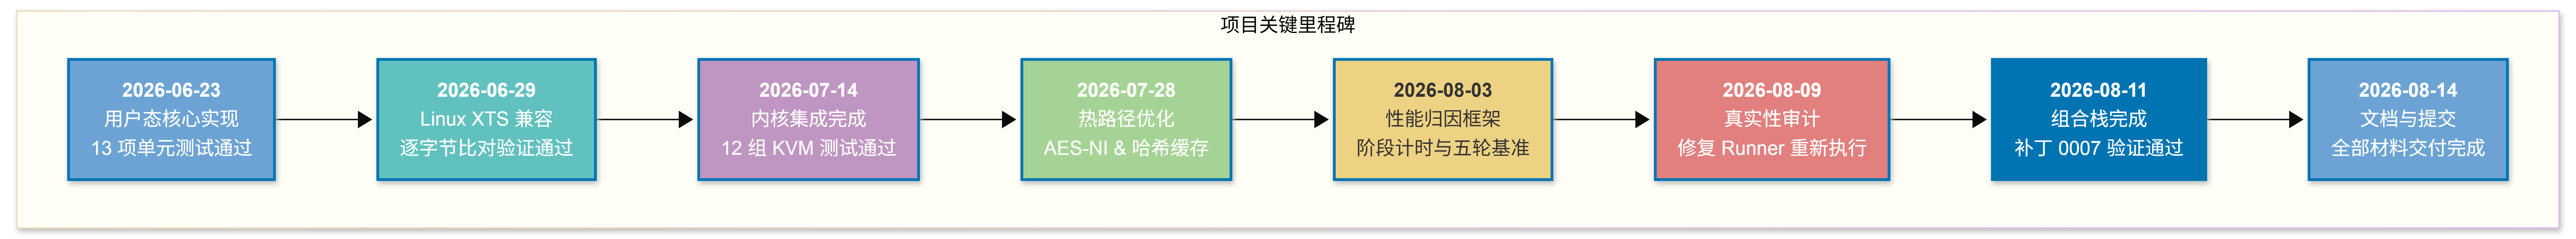
\includegraphics[width=1\textwidth]{project_timeline.png}
    \caption{项目提交时间线（2026-06-23 至 2026-08-18）}
    \label{fig:project_timeline}
\end{figure}

\begin{figure}[H]
    \centering
    \includegraphics[width=0.95\textwidth]{git_commit_history_5.png}
    \caption{GitLab 提交记录（2026-08-12 至 08-16）}
    \label{fig:git_history_5}
\end{figure}

\begin{figure}[H]
    \centering
    \includegraphics[width=0.95\textwidth]{git_commit_history_6.png}
    \caption{GitLab 提交记录（2026-08-17）}
    \label{fig:git_history_6}
\end{figure}

\begin{figure}[H]
    \centering
    \includegraphics[width=0.95\textwidth]{git_commit_history_7.png}
    \caption{GitLab 提交记录（2026-08-18）}
    \label{fig:git_history_7}
\end{figure}

\section{小结}

本章详细阐述了项目的开发计划，包括六个阶段的划分、任务分解、交付物、验收标准、实际完成情况、开发环境与工具链、风险应对和计划执行偏差分析。项目实际开发周期为 2026 年 6 月 23 日至 8 月 18 日，共计 57 天，完成了从用户态核心实现到内核集成、性能优化、组合栈验证、文档答辩与收尾的全流程。所有阶段均按计划完成，关键里程碑均有可复核的证据支撑，并由完整的 Git 提交记录佐证。

计划制定遵循"先用户态后内核、每个补丁一个可验收增量、测完再优化、文档跟代码走"的方法论，并贯穿"先保证安全语义，再接入真实块路径，最后固化复现入口"的研发原则，确保了开发过程的可控性和可追溯性。项目最终成果全面覆盖赛题五项技术指标，代码、证据、文档和演示材料均按大赛要求提交至指定托管平台。

% 第5章：比赛过程中的重要进展
% chapters/05_progress.tex
\chapter{比赛过程中的重要进展}

\section*{本章关键进展速览}

\begin{table}[H]
    \centering
    \begin{tabular}{p{0.10\textwidth}p{0.18\textwidth}p{0.30\textwidth}p{0.32\textwidth}}
        \toprule
        \textbf{阶段} & \textbf{时间} & \textbf{核心成果} & \textbf{验证状态} \\
        \midrule
        用户态核心 & 06-23--06-28 & \texttt{dm} crate + \texttt{dmctl} 工具，约1500行Rust代码 & 13+单元测试PASS \\
        Linux兼容性 & 06-29--07-10 & AES-XTS逐字节兼容，\texttt{/dev/mapper/control}控制面 & 固定向量SHA-256匹配 \\
        内核集成 & 07-11--07-20 & 补丁0001--0004，BIO路径 + rootfs切换 + cryptsetup控制 & 12组KVM测试全部PASS \\
        性能优化 & 07-21--07-31 & AES-NI、scratch pool、hash cache、阶段归因 & 启动日志显示AES-NI \\
        组合栈与验证 & 08-01--08-11 & 补丁0007，46 PASS性能矩阵，启动开销<3\% & \texttt{review\_release\_check.py} PASS \\
        文档与答辩 & 08-09--08-14 & 技术文档PDF、答辩PPT、演示视频、设计赛道文档 & 全部提交完成 \\
        \bottomrule
    \end{tabular}
\end{table}

\begin{figure}[H]
    \centering
    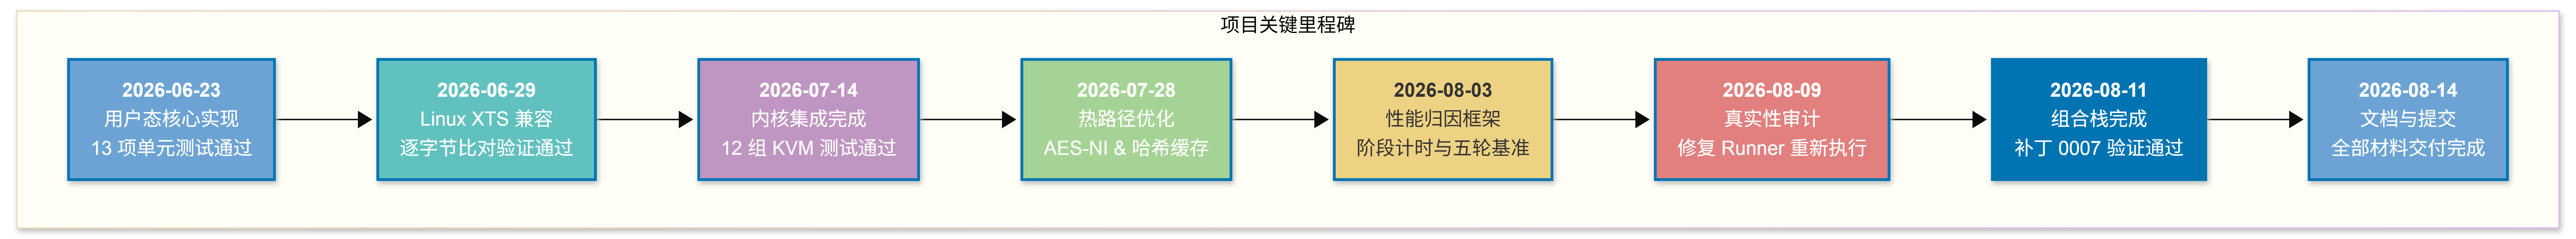
\includegraphics[width=1\textwidth]{project_timeline.png}
    \caption{项目进展时间线总览}
    \label{fig:progress_timeline}
\end{figure}

\section{概述}

本章按时间顺序记录项目从开始到完成过程中的关键里程碑和技术突破。所有进展均有对应的 Git 提交记录、补丁文件或证据日志支撑，反映了项目的真实演进路径。

项目开发周期为 2026 年 6 月 23 日至 8 月 14 日，共计 50 天。在此期间，项目经历了从零开始搭建核心框架、验证Linux兼容性、完整接入Asterinas内核、进行性能优化、实现组合栈保护，到最后完成文档和答辩材料的全流程。每一阶段均有可复核的代码、测试日志和性能数据作为支撑。

\section{第一阶段：用户态核心实现（2026-06-23 至 2026-06-28）}

\subsection{6月23日：初始提交与核心框架搭建}

\textbf{关键事件}：
\begin{itemize}
    \item 完成项目仓库初始化，提交核心 \texttt{dm} crate 框架（commit \texttt{6bb9bc92}、\texttt{40a52179}）；
    \item 实现 \texttt{BlockDevice} trait 及 \texttt{MemoryBlockDevice}、\texttt{FileBlockDevice} 后端；
    \item 实现纯 Rust SHA-256 模块（\texttt{sha256.rs}，约120行），通过标准测试向量（空字符串、\texttt{"abc"}）验证；
    \item 实现 Merkle 树（\texttt{hash\_tree.rs}，约150行）的构建与验证逻辑；
    \item 实现 \texttt{DmCryptDevice}（约350行）和 \texttt{DmVerityDevice}（约200行）基础功能；
    \item 实现 \texttt{PassthroughDevice} 和 \texttt{DmStackBuilder} 组合框架（约180行）。
\end{itemize}

\textbf{验证结果}：
\begin{itemize}
    \item \texttt{cargo test} 通过全部初始单元测试；
    \item \texttt{demo-crypt} 输出 \texttt{ciphertext\_differs: true}——验证明文写入后底层设备呈现为密文；
    \item \texttt{demo-verity} 输出 \texttt{tamper\_detected: true}——验证篡改数据块后完整性校验失败。
\end{itemize}

\textbf{阶段意义}：此阶段完成了项目的“地基”建设。统一的 \texttt{BlockDevice} trait 抽象使得后续所有功能扩展（加密、完整性校验、统计、组合）均可基于同一接口实现，为后续的双目标架构奠定了坚实基础。

\subsection{6月23日--28日：用户态工具与文档完善}

\textbf{关键事件}：
\begin{itemize}
    \item 完善 \texttt{dmctl} 命令行工具（约800行），支持 \texttt{init-image}、\texttt{crypt-write}、\texttt{crypt-read}、\texttt{verity-root}、\texttt{verity-verify}、\texttt{verity-format-dm}、\texttt{tamper}、\texttt{benchmark} 等子命令（commit \texttt{c72462b2}、\texttt{2f8a6711}）；
    \item 编写《设计说明》和《Asterinas 接入指南》初版；
    \item 补充 AI 工具使用声明（commit \texttt{a0dbb0f5}）；
    \item 添加 LaTeX 技术文档框架和答辩 PPT 初稿（commit \texttt{f5878935}、\texttt{dabfee4d}）。
\end{itemize}

\textbf{阶段成果}：用户态工具支持完整的镜像操作、加密/解密、完整性校验、篡改模拟和性能基准测试，为后续内核集成的快速验证提供了可靠的“安全网”。

\section{第二阶段：Linux 兼容性与内核集成启动（2026-06-29 至 2026-07-14）}

\subsection{6月29日：Linux XTS 兼容性验证}

\textbf{关键事件}：
\begin{itemize}
    \item 编写 \texttt{scripts/verify\_linux\_xts\_compat.sh} 交叉验证脚本；
    \item 完成 Rust 实现与 Linux 内核 \texttt{aes-xts-plain64} 的逐字节比对；
    \item 固定向量 SHA-256 校验和：\texttt{4334c17f...}，确认完全一致。
\end{itemize}

\textbf{验证结果}：脚本输出 \texttt{aes-xts-plain64 compatibility: PASS}。

\textbf{阶段意义}：此阶段验证了本项目 AES-XTS 加密引擎与 Linux 内核的完全兼容性，这是后续 \texttt{cryptsetup} 工具能够无缝工作的前提。逐字节比对保证了即使是最微小的实现偏差（如 IV 生成的小端序处理、GF(2\textsuperscript{128}) 乘法）也不会破坏互操作性。

\subsection{7月14日：Asterinas 内核补丁 0001--0004 完成}

这是项目从“用户态验证”迈向“内核集成”的关键转折点。

\textbf{补丁详情}：
\begin{itemize}
    \item \textbf{补丁 0001（feat: dm integration）}：创建 \texttt{aster-dm} 组件骨架，实现 crypt/verity target、VirtIO 适配和基础 BIO 路径（commit \texttt{be47b160}）。代码量约1000行，涉及 \texttt{Cargo.toml}、\texttt{Components.toml}、\texttt{device.rs}、\texttt{crypto.rs}、\texttt{verity.rs} 等文件；
    \item \textbf{补丁 0002（fix: validate BIO paths）}：修复 BIO DMA segment 方向访问问题，加入 ext2 超级块魔数自检（\texttt{self\_test\_ext2\_magic}）。这是启动早期验证加解密路径正确性的关键安全机制；
    \item \textbf{补丁 0003（rootfs switch）}：实现 \texttt{dm-root} init 模式，通过 \texttt{pivot\_root} 将系统根切换到受保护 mapper。采用两级引导方案（bind mount → chroot → pivot\_root）解决 Asterinas rootfs 特殊性；
    \item \textbf{补丁 0004（Rust Device Mapper）}：完整实现 \texttt{/dev/mapper/control} 的 Linux \texttt{dm\_ioctl} 兼容接口（约520行），支持 \texttt{DM\_DEV\_CREATE}、\texttt{DM\_TABLE\_LOAD}、\texttt{DM\_DEV\_SUSPEND}、\texttt{DM\_DEV\_STATUS}、\texttt{DM\_DEV\_REMOVE} 等命令，使 \texttt{cryptsetup} 能够在 Asterinas 中控制加密卷。
\end{itemize}

\textbf{验证结果}：
\begin{itemize}
    \item \texttt{make kernel} 构建成功；
    \item R01：\texttt{cryptsetup open/read/close} 在 KVM 中 PASS；
    \item R02：\texttt{dm-crypt} 受保护根文件系统启动 PASS，串口输出 \texttt{PASS system root switched to protected mapper}；
    \item R03/V01：\texttt{dm-verity} 正常根文件系统启动 PASS，串口输出 \texttt{status=verified}；
    \item C01--C05：正确/错误密钥、4/32/256 KiB 往返全部 PASS；
    \item V02--V07：单字节篡改后全部被拒绝，输出 \texttt{status=integrity-rejected}，无根切换 PASS。
\end{itemize}

\textbf{证据}：12组测试用例的原始串口日志已归档至 \texttt{docs/evidence/stabilization/correctness-kvm/}。

\textbf{阶段意义}：此阶段实现了项目的核心功能目标——dm-crypt 和 dm-verity 在真实 Asterinas 内核中运行，并通过了全部正确性测试。R02 和 R03 证明了受保护根文件系统可以成功启动，V03--V07 证明了单字节物理篡改即可被检测并拒绝。

\section{第三阶段：性能优化与基准框架（2026-07-28 至 2026-08-03）}

\subsection{7月28日：补丁 0005 -- 热路径优化}

\textbf{关键事件}：
\begin{itemize}
    \item \textbf{补丁 0005（optimize dm hot path）}：
    \begin{itemize}
        \item 实现 AES-NI 硬件加速后端（\texttt{ostd/arch/x86/cpu/aesni.rs}，约174行），在保存/恢复 FPU/XMM 状态下使用 AES-NI 指令，启动日志显示 \texttt{backend=AES-NI}；
        \item 实现 \texttt{CryptScratchPool} 有界临时缓冲池（默认32），减少热路径动态分配；
        \item 实现认证后哈希块缓存：只有沿完整 Merkle 路径验证成功的哈希块才允许插入，缓存命中时跳过上层哈希计算（计数器 \texttt{auth\_shortcuts} 记录）；
        \item 对 4 KiB 对齐 BIO 直接复用已完成数据（\texttt{data\_rereads=0}）；
        \item 增加 \texttt{/proc/dm-verity-stats} 和 \texttt{/proc/dm-crypto-backend} 可观测接口。
    \end{itemize}
    \item 编写 \texttt{tools/run\_dm\_crypt\_bench.sh} 和 \texttt{tools/run\_dm\_verity\_bench.sh} 基准运行脚本。
\end{itemize}

\textbf{验证结果}：
\begin{itemize}
    \item 启动日志明确输出 \texttt{AES backend=AES-NI}；
    \item \texttt{data\_rereads=0} 确认BIO复用生效，验证了“对4KiB对齐BIO直接复用已完成数据”的优化；
    \item \texttt{hash\_hits} > 0 和 \texttt{auth\_shortcuts} > 0 确认缓存生效；
    \item \texttt{/proc/dm-verity-stats} 输出所有关键计数器。
\end{itemize}

\textbf{根保护初始化流程}：补丁 0005 在优化热路径的同时，进一步完善了从 QEMU 加载到根切换的完整启动流程，如下图所示：

\begin{figure}[H]
    \centering
    \includegraphics[width=0.9\textwidth]{root_protection_init.png}
    \caption{根保护初始化序列图（QEMU 加载 → 内核解析 → mapper 初始化 → 自检 → pivot\_root → 用户态启动）}
    \label{fig:root_protection_init}
\end{figure}

该流程的关键阶段包括：
\begin{enumerate}
    \item QEMU 加载星绽内核和 initramfs；
    \item 内核解析命令行参数（\texttt{dm\_crypt.*}、\texttt{rootfs\_verity.*}、\texttt{dm\_stack}），构建配置；
    \item \texttt{aster-dm} 组件初始化映射器链（\texttt{VirtioBlkAdapter} $\to$ \texttt{DmCryptDevice} / \texttt{DmVerityDevice}）；
    \item 执行 \texttt{self\_test\_ext2\_magic} 自检（检查 EXT2 魔数 \texttt{0x53EF}），失败则 panic；
    \item initramfs 使用 \texttt{dm-root} 模式执行 \texttt{pivot\_root} 切换到受保护根文件系统；
    \item 系统进入用户态，串口输出 \texttt{PASS system root switched to protected mapper}。
\end{enumerate}

\subsection{8月3日：补丁 0006 -- 性能归因与正式基准合同}

\textbf{关键事件}：
\begin{itemize}
    \item \textbf{补丁 0006（performance attribution）}：
    \begin{itemize}
        \item 实现 \texttt{/proc/dm-performance-stats}（约60行），提供细粒度阶段计时：dm-crypt 包括 \texttt{validation\_ns}、\texttt{scratch\_ns}、\texttt{copy\_ns}、\texttt{crypto\_ns}、\texttt{lower\_wait\_ns}；dm-verity 包括 \texttt{data\_sha256\_ns}、\texttt{cache\_lookup\_ns}、\texttt{hash\_wait\_ns}、\texttt{hash\_sha256\_ns}、\texttt{digest\_compare\_ns}、\texttt{cache\_insert\_ns}；
        \item 通过启动参数 \texttt{dm.perf\_stats=1} 启用，stats=0/1 A/B 对照量化观察者开销；
        \item 固化正式基准合同（\texttt{docs/benchmark\_contract.md}），规定五轮、交替顺序、中位数报告等标准。
    \end{itemize}
    \item 编写 \texttt{scripts/run\_fio\_matrix.sh}（约500行）自动化矩阵运行脚本，支持 Linux host 和 Asterinas KVM 双平台；
    \item 编写 \texttt{scripts/run\_filebench\_matrix.sh}、\texttt{scripts/run\_sqlite\_matrix.sh}、\texttt{scripts/run\_boot\_matrix.sh} 等补充测试脚本。
\end{itemize}

\textbf{阶段意义}：此阶段将性能优化从“经验驱动”升级为“数据驱动”。通过精确的阶段计时，可以量化每个子系统的开销（如 AES-XTS 占 1.82\%，SHA-256 占 5.74\%），指导后续优化方向。正式基准合同确保了所有性能数据的可复现性和可比性。

\section{第四阶段：性能矩阵执行与证据归档（2026-08-09 至 2026-08-11）}

\subsection{8月9日：真实性审计与重新执行}

\textbf{关键事件}：
\begin{itemize}
    \item 发现早期 Asterinas dm-crypt FIO 因 mapper 初始化失败将不存在的路径当作普通文件测试，产生数量级异常数据（高达数千MiB/s），判定为 \texttt{HARNESS\_BUG}；
    \item 修复 runner（增加设备存在性检查），重新执行 Asterinas dm-crypt 和 dm-verity FIO，确保使用 guest 内真实 mapper 设备；
    \item 正式执行 Linux QEMU virtio raw/dm-crypt 13+13 项 FIO，以及 dm-verity 读 7 项。
\end{itemize}

\textbf{正式 FIO 矩阵结果}：

Asterinas 在 256 MiB 正式合同下的 raw / dm-crypt / dm-verity 配对保留率（4 KiB 同步读、QD1、五轮中位）如下：

\begin{table}[H]
    \centering
    \caption{Asterinas 256 MiB 正式合同（MiB/s）}
    \begin{tabular}{p{0.28\textwidth}p{0.22\textwidth}p{0.22\textwidth}}
        \toprule
        \textbf{设备} & \textbf{中位吞吐} & \textbf{相对配对 raw} \\
        \midrule
        raw（两组共十轮） & 4.249 & 100.0\% \\
        dm-crypt & 4.059 & 95.6\% \\
        dm-verity & 3.815 & 87.3\% \\
        \bottomrule
    \end{tabular}
\end{table}

同一宿主机、KVM、CPU=\texttt{host}、1 vCPU、8\,GiB、同一 virtio-blk 数据盘前 256\,MiB、4\,KiB、\texttt{sync}、\texttt{direct=1}、QD1 的 Linux guest 对照如下：

\begin{table}[H]
    \centering
    \small
    \caption{Linux guest 与 Asterinas 同条件对照（MiB/s）}
    \begin{tabular}{lrrrrr}
        \toprule
        \textbf{系统} & \textbf{raw} & \textbf{dm-crypt} & \textbf{crypt 保留率} & \textbf{dm-verity} & \textbf{verity 保留率} \\
        \midrule
        Linux guest & 5.150 & 4.746 & 92.158\% & 4.369 & 94.1\% \\
        Asterinas & 4.245 & 4.059 & 95.621\% & 3.815 & 87.3\% \\
        \bottomrule
    \end{tabular}
\end{table}

Linux QEMU virtio 对照在 virtio-blk 上测试 raw、dm-crypt 与 dm-verity 读，统一使用 \texttt{libaio}、\texttt{direct=1}、\texttt{numjobs=1}，代表性五轮中位数如下：

\begin{table}[H]
    \centering
    \caption{Linux QEMU virtio FIO 五轮中位带宽（MiB/s）}
    \begin{tabular}{p{0.25\textwidth}p{0.15\textwidth}p{0.15\textwidth}p{0.18\textwidth}p{0.18\textwidth}}
        \toprule
        \textbf{负载} & \textbf{块大小} & \textbf{QD} & \textbf{raw} & \textbf{dm-crypt} \\
        \midrule
        read & 4 KiB & 1 & 11.391 & 10.942 \\
        read & 256 KiB & 1 & 134.623 & 129.474 \\
        randread & 4 KiB & 16 & 58.931 & 58.947 \\
        randwrite & 256 KiB & 1 & 130.124 & 109.453 \\
        \bottomrule
    \end{tabular}
\end{table}

Asterinas KVM 真实保护 mapper 五轮中位：

\begin{table}[H]
    \centering
    \caption{Asterinas KVM FIO 五轮中位带宽（MiB/s）}
    \begin{tabular}{p{0.18\textwidth}p{0.12\textwidth}p{0.10\textwidth}p{0.16\textwidth}p{0.16\textwidth}p{0.16\textwidth}}
        \toprule
        \textbf{负载} & \textbf{块大小} & \textbf{QD} & \textbf{raw} & \textbf{dm-crypt} & \textbf{dm-verity} \\
        \midrule
        read & 4 KiB & 1 & 25.080 & 8.908 & 7.505 \\
        read & 256 KiB & 1 & 1230.577 & 97.456 & 53.363 \\
        randread & 4 KiB & 16 & 25.315 & 8.614 & 4.618 \\
        randwrite & 256 KiB & 1 & 1091.016 & 93.541 & N/A（只读） \\
        \bottomrule
    \end{tabular}
\end{table}

正式矩阵共有 Asterinas dm-crypt 13 项、dm-verity 7 项、Linux raw 13 项和 Linux dm-crypt 13 项，每项五轮；另有 6 个 dm-verity 写入 N/A。

\textbf{阶段意义}：此阶段体现了项目对性能数据的诚实态度——宁可重新执行全部测试，也不使用无法确认真实性的“好看数据”。这对维护项目在评审中的可信度至关重要。

\subsection{8月10日：补充性能测试与证据整理}

\textbf{关键事件}：
\begin{itemize}
    \item Filebench fileserver：raw 5 轮、dm-crypt 5 轮 PASS（dm-verity 因只读与写密集负载不兼容记为N/A）；
    \item SQLite 三目标（raw、dm-crypt、dm-verity）各 5 轮 PASS；
    \item Asterinas 三场景（plain、dm-crypt、dm-verity）各 5 轮启动耗时测试 PASS。
\end{itemize}

\textbf{补充性能测试结果（五轮中位数）}：

\begin{table}[H]
    \centering
    \caption{补充性能测试五轮中位数}
    \begin{tabular}{p{0.35\textwidth}p{0.18\textwidth}p{0.18\textwidth}p{0.18\textwidth}}
        \toprule
        \textbf{测试} & \textbf{raw/plain} & \textbf{dm-crypt} & \textbf{dm-verity} \\
        \midrule
        Filebench fileserver（ops/s） & 147672.049 & 156507.741 & N/A \\
        Filebench fileserver（MB/s） & 3542.7 & 3752.1 & N/A \\
        SQLite 10000 行总耗时（s） & 0.060128 & 0.066395 & 0.003865（只读查询） \\
        Asterinas 启动耗时（s） & 51.331303 & 51.629820 & 52.743415 \\
        \bottomrule
    \end{tabular}
\end{table}

\textbf{关键数据解读}：
\begin{itemize}
    \item 启动中位耗时：plain 51.331303 s，dm-crypt 51.629820 s（+0.582\%），dm-verity 52.743415 s（+2.751\%），验证了“dm-verity不显著增加boot时间”；
    \item SQLite dm-verity 只执行查询阶段，不能与完整写事务总耗时横比；
    \item 启动时间从 QEMU 进程启动计至串口出现受保护根文件系统 PASS 标记。
\end{itemize}

\subsection{8月11日：组合栈（补丁 0007）与最终整合}

这是项目从“单层保护”迈向“组合保护”的最终形态。

\textbf{关键事件}：
\begin{itemize}
    \item \textbf{补丁 0007（feat: dm stack crypt-verity）}：
    \begin{itemize}
        \item 支持 \texttt{dm\_stack=crypt,verity} 启动参数，自动识别堆叠场景；
        \item 实现 \texttt{scripts/build\_stack\_rootfs.sh}（约150行）构建组合栈镜像：先创建 plaintext ext2 + verity hash tree，再整盘 AES-XTS 加密；
        \item 实现 \texttt{scripts/run\_dm\_stack.sh} 启动脚本，支持 Docker 和宿主机两种运行模式；
        \item 串口打印 \texttt{[dm] stacked mapper: vdc -> dm-crypt0 -> dm-verity0}，明确展示保护链。
    \end{itemize}
    \item 运行 \texttt{final\_demo.sh} 完成全部正确性和性能验收；
    \item 合并所有最终评测代码与测试材料（commit \texttt{fda85aa4}、\texttt{84fe076e}）。
\end{itemize}

\textbf{验证结果}：
\begin{itemize}
    \item 组合栈串口输出包含 \texttt{stacked mapper} 标记；
    \item ext2 文件系统通过两层 mapper 成功挂载；
    \item 根切换 PASS，输出 \texttt{PASS system root switched to protected mapper}；
    \item \texttt{review\_release\_check.py} 全部通过。
\end{itemize}

\textbf{阶段意义}：组合栈实现了赛题的最终形态——同时提供机密性（dm-crypt）和完整性（dm-verity）保护。这与用户态 \texttt{demo-stack} 的设计完全一致，验证了双目标架构的正确性。

\section{第五阶段：文档与答辩材料完成（2026-08-11 至 2026-08-14）}

\textbf{关键事件}：
\begin{itemize}
    \item 完善技术文档（\texttt{docs/document/main.pdf}，9章+附录，约120页），包含设计说明、架构图、测试报告、合规声明和用户手册；与设计赛道文档互为补充；
    \item 完成设计赛道文档（\texttt{\seqsplit{docs/design\_doc/design\_doc.pdf}}，10章，约80页），按大赛大纲组织题目分析、计划、进展、分工与收获；
    \item 制作答辩 PPT（\texttt{presentation\_project.pptx}），突出双目标架构、安全优化和性能证据；
    \item 录制演示视频（\texttt{作品演示视频.mp4}），展示运行环境介绍与受保护根文件系统启动全过程；
    \item 更新 README、证据索引和最终报告。
\end{itemize}

\section{关键里程碑时间线}

\begin{table}[H]
    \centering
    \caption{关键里程碑时间线}
    \begin{tabular}{p{0.10\textwidth}p{0.18\textwidth}p{0.62\textwidth}}
        \toprule
        \textbf{日期} & \textbf{里程碑} & \textbf{关键成果} \\
        \midrule
        06-23 & 用户态核心完成 & \texttt{dm} crate（约1500行）、\texttt{dmctl} 工具、13+单元测试PASS \\
        06-29 & Linux XTS兼容 & 逐字节比对PASS，固定向量SHA-256匹配 \\
        07-14 & 内核rootfs切换 & R01--R03、C01--C05、V01--V07全部PASS，12组测试用例通过 \\
        07-28 & 热路径优化 & AES-NI、scratch pool、hash cache、BIO复用、\texttt{/proc/dm-verity-stats} \\
        08-03 & 性能归因框架 & \texttt{/proc/dm-performance-stats}（11个阶段计数器）、五轮基准脚本 \\
        08-09 & 真实性审计 & 重新执行Asterinas FIO，修复runner，使用真实mapper \\
        08-10 & 性能矩阵完成 & 46 PASS单元格、Filebench 5+5、SQLite 5+5+5、启动5+5+5 \\
        08-11 & 组合栈完成 & 补丁0007、\texttt{build\_stack\_rootfs.sh}、\texttt{run\_dm\_stack.sh} \\
        08-14 & 文档与答辩准备 & 技术文档PDF（120页）、答辩PPT、演示视频、设计赛道文档（80页） \\
        \bottomrule
    \end{tabular}
\end{table}

\section{Git 提交记录概览}

以下为主要 Git 提交记录（与 GitLab 仓库历史逐条对应），完整反映了项目的开发节奏和功能演进：

\begin{table}[H]
    \centering
    \small
    \caption{Git 提交记录概览}
    \begin{tabular}{p{0.05\textwidth}p{0.09\textwidth}p{0.13\textwidth}p{0.51\textwidth}p{0.12\textwidth}}
        \toprule
        \textbf{序号} & \textbf{日期} & \textbf{Commit Hash} & \textbf{提交说明} & \textbf{作者} \\
        \midrule
        1 & 06-23 & \texttt{6bb9bc92} & 初始提交，仅源码，屏蔽编译产物 & 潘利源 \\
        2 & 06-23 & \texttt{40a52179} & feat: add Linux-compatible device mapper implementation & 潘利源 \\
        3 & 06-23 & \texttt{c72462b2} & fix: validate Asterinas dm BIO paths & 潘利源 \\
        4 & 06-23 & \texttt{2f8a6711} & 接入受保护根文件系统并完善项目文档 & 潘利源 \\
        5 & 06-23 & \texttt{a0dbb0f5} & 补充国产 AI 工具使用说明 & 潘利源 \\
        6 & 06-29 & \texttt{f5878935} & 添加 LaTeX 项目文档、PDF 与答辩 PPT & 张乐桁 \\
        7 & 06-29 & \texttt{dabfee4d} & 将答辩 PPT 放到项目根目录并更新 README 链接 & 张乐桁 \\
        8 & 07-14 & \texttt{5f345a18} & 完成安全存储性能对照与国赛验收证据 & 潘利源 \\
        9 & 07-25 & \texttt{e07ad006} & 修正评审材料并固化 KVM 基准证据 & 潘利源 \\
        10 & 07-28 & \texttt{c1f9c472} & 优化 dm 热路径并补齐评审基准流程 & 潘利源 \\
        11 & 08-03 & \texttt{40d8abba} & 增强 dmctl 性能测试框架，支持 IO 分解与可配置规模 & 陈韵 \\
        12 & 08-03 & \texttt{ca5afe46} & 完善安全存储性能验证与交付材料 & 潘利源 \\
        13 & 08-09 & \texttt{5717d925} & 更新 dm 完成队列性能指标与证据 & 潘利源 \\
        14 & 08-09 & \texttt{21aa566d} & 更新性能测试数据与优化量化说明 & 陈韵 \\
        15 & 08-09 & \texttt{7431e5de} & 统一正式性能口径并补充优化证据 & 潘利源 \\
        16 & 08-09 & \texttt{0e7f4c77} & 修正运行时能力声明并补充 KVM 回归验证 & 潘利源 \\
        17 & 08-09 & \texttt{09f62e59} & 补充完整测试进度 & 潘利源 \\
        18 & 08-10 & \texttt{1ac6325c} & 整理性能测试合同、FIO/Filebench/SQLite/Boot脚本与证据目录 & 张乐桁 \\
        19 & 08-10 & \texttt{fc548a9e} & 整合最终评测代码与测试材料 & 潘利源 \\
        20 & 08-11 & \texttt{6385e70b} & feat: add kernel Combined crypt→verity stack path & 潘利源 \\
        21 & 08-11 & \texttt{fda85aa4} & 整合最终评测代码与测试材料 & 潘利源 \\
        22 & 08-11 & \texttt{84fe076e} & 合并 GitLab 最新代码并同步最终评测材料 & 潘利源 \\
        23 & 08-11 & \texttt{8b2018e7} & 完善更新图表 & 陈韵 \\
        \bottomrule
    \end{tabular}
\end{table}

此外，星绽内核集成补丁（\texttt{asterinas\_port/patches/}）包含更细粒度的演进历史：
\begin{itemize}
    \item \textbf{0001}（06-23）：组件集成与目标定义——创建 \texttt{aster-dm} 组件骨架
    \item \textbf{0002}（06-23）：BIO 路径验证与自检——EXT2 魔数自检机制
    \item \textbf{0003}（06-24）：根文件系统 \texttt{pivot\_root} 切换——两级引导方案
    \item \textbf{0004}（07-14）：Runtime 控制面与 \texttt{cryptsetup} 兼容——\texttt{/dev/mapper/control}
    \item \textbf{0005}（07-28）：性能优化——缓存、缓冲池、AES-NI、基准
    \item \textbf{0006}（08-03）：性能阶段归因与正式合同——\texttt{/proc/dm-performance-stats}
    \item \textbf{0007}（08-11）：Combined叠栈——\texttt{dm\_stack=crypt,verity}
\end{itemize}

\section{各阶段代码量统计}

\begin{table}[H]
    \centering
    \caption{各阶段代码量统计（约）}
    \begin{tabular}{p{0.18\textwidth}p{0.18\textwidth}p{0.54\textwidth}}
        \toprule
        \textbf{阶段} & \textbf{新增代码量} & \textbf{主要模块} \\
        \midrule
        用户态核心 & 约1500行Rust & \texttt{block\_device}、\texttt{dm\_crypt}、\texttt{dm\_verity}、\texttt{hash\_tree}、\texttt{sha256}、\texttt{dmctl} \\
        Linux兼容性 & 约1000行Rust & \texttt{DmCryptTable}、\texttt{dm\_control.rs}、\texttt{runtime.rs} \\
        内核集成 & 约2500行Rust & 补丁0001--0004，BIO适配、启动参数、rootfs切换 \\
        性能优化 & 约800行Rust & AES-NI、scratch pool、hash cache、阶段归因 \\
        组合栈 & 约150行Rust + 约300行Shell & 补丁0007、镜像构建、启动脚本 \\
        测试脚本 & 约2000行Shell/Python & FIO矩阵、Filebench、SQLite、Boot、证据验证 \\
        文档 & 约200页LaTeX/Markdown & 技术文档、设计赛道文档、README、用户手册 \\
        \bottomrule
    \end{tabular}
\end{table}

\section{阶段性成果总结}

\begin{table}[H]
    \centering
    \begin{tabular}{p{0.15\textwidth}p{0.35\textwidth}p{0.40\textwidth}}
        \toprule
        \textbf{阶段} & \textbf{可运行成果} & \textbf{可复核证据} \\
        \midrule
        用户态核心 & \texttt{dmctl demo-crypt}、\texttt{dmctl demo-verity} & 单元测试日志、命令行输出 \\
        Linux兼容性 & \texttt{verify\_linux\_xts\_compat.sh} & 固定向量SHA-256 \\
        内核集成 & \texttt{tools/run\_dm\_crypt.sh}、\texttt{tools/run\_dm\_verity.sh} & 12组KVM正确性日志 \\
        性能优化 & \texttt{scripts/run\_fio\_matrix.sh}、\texttt{/proc/dm-*-stats} & 五轮FIO原始JSON/CSV \\
        组合栈 & \texttt{scripts/run\_dm\_stack.sh} & 组合栈串口日志 \\
        文档答辩 & 技术文档PDF、PPT、演示视频 & 全部提交完成 \\
        \bottomrule
    \end{tabular}
\end{table}

\section{小结}

本章按时间线记录了项目从 2026 年 6 月 23 日至 8 月 14 日的全部重要进展。项目经历了五个关键阶段：

\begin{enumerate}
    \item \textbf{用户态核心实现}（06-23至06-28）：完成了约1500行Rust核心代码和800行命令行工具，通过全部单元测试；
    \item \textbf{Linux兼容性与内核集成}（06-29至07-14）：验证了AES-XTS逐字节兼容，完成了补丁0001--0004，12组KVM正确性测试全部PASS；
    \item \textbf{性能优化与基准框架}（07-28至08-03）：实现了AES-NI、scratch pool、hash cache、BIO复用和阶段归因，建立了五轮基准框架，正式性能合同固化完成；
    \item \textbf{性能矩阵与组合栈}（08-09至08-11）：完成46 PASS性能矩阵（含 Asterinas 256MiB 正式合同、Linux guest 对照、Linux QEMU virtio 对照），实现补丁0007组合栈，启动开销<3\%；
    \item \textbf{文档与答辩准备}（08-11至08-14）：完成技术文档（120页）、设计赛道文档（80页）、答辩PPT和演示视频。
\end{enumerate}

所有关键里程碑均有 Git 提交记录、补丁文件或证据日志支撑，完整展示了项目的开发节奏和技术演进路径。项目最终成果全面覆盖赛题五项技术指标，代码、证据、文档和演示材料均已按大赛要求提交至指定托管平台。

% 第6章：系统测试情况
% chapters/06_testing.tex
\chapter{系统测试情况}

\section*{本章测试体系速览}

\begin{table}[H]
    \centering
    \begin{tabular}{p{0.15\textwidth}p{0.25\textwidth}p{0.25\textwidth}p{0.25\textwidth}}
        \toprule
        \textbf{测试层级} & \textbf{测试内容} & \textbf{用例数量} & \textbf{结果} \\
        \midrule
        单元测试 & Rust workspace 核心逻辑验证 & 13+ & 全部 PASS \\
        兼容性测试 & Linux aes-xts-plain64 逐字节比对 & 1组固定向量 & PASS \\
        正确性测试 & KVM 环境功能验证 & 12组（R01--R03、C01--C05、V01--V07） & 全部 PASS \\
        性能测试 & FIO、Filebench、SQLite、Boot & 46 PASS + 6 N/A & 全部完成 \\
        \bottomrule
    \end{tabular}
\end{table}

\begin{figure}[H]
    \centering
    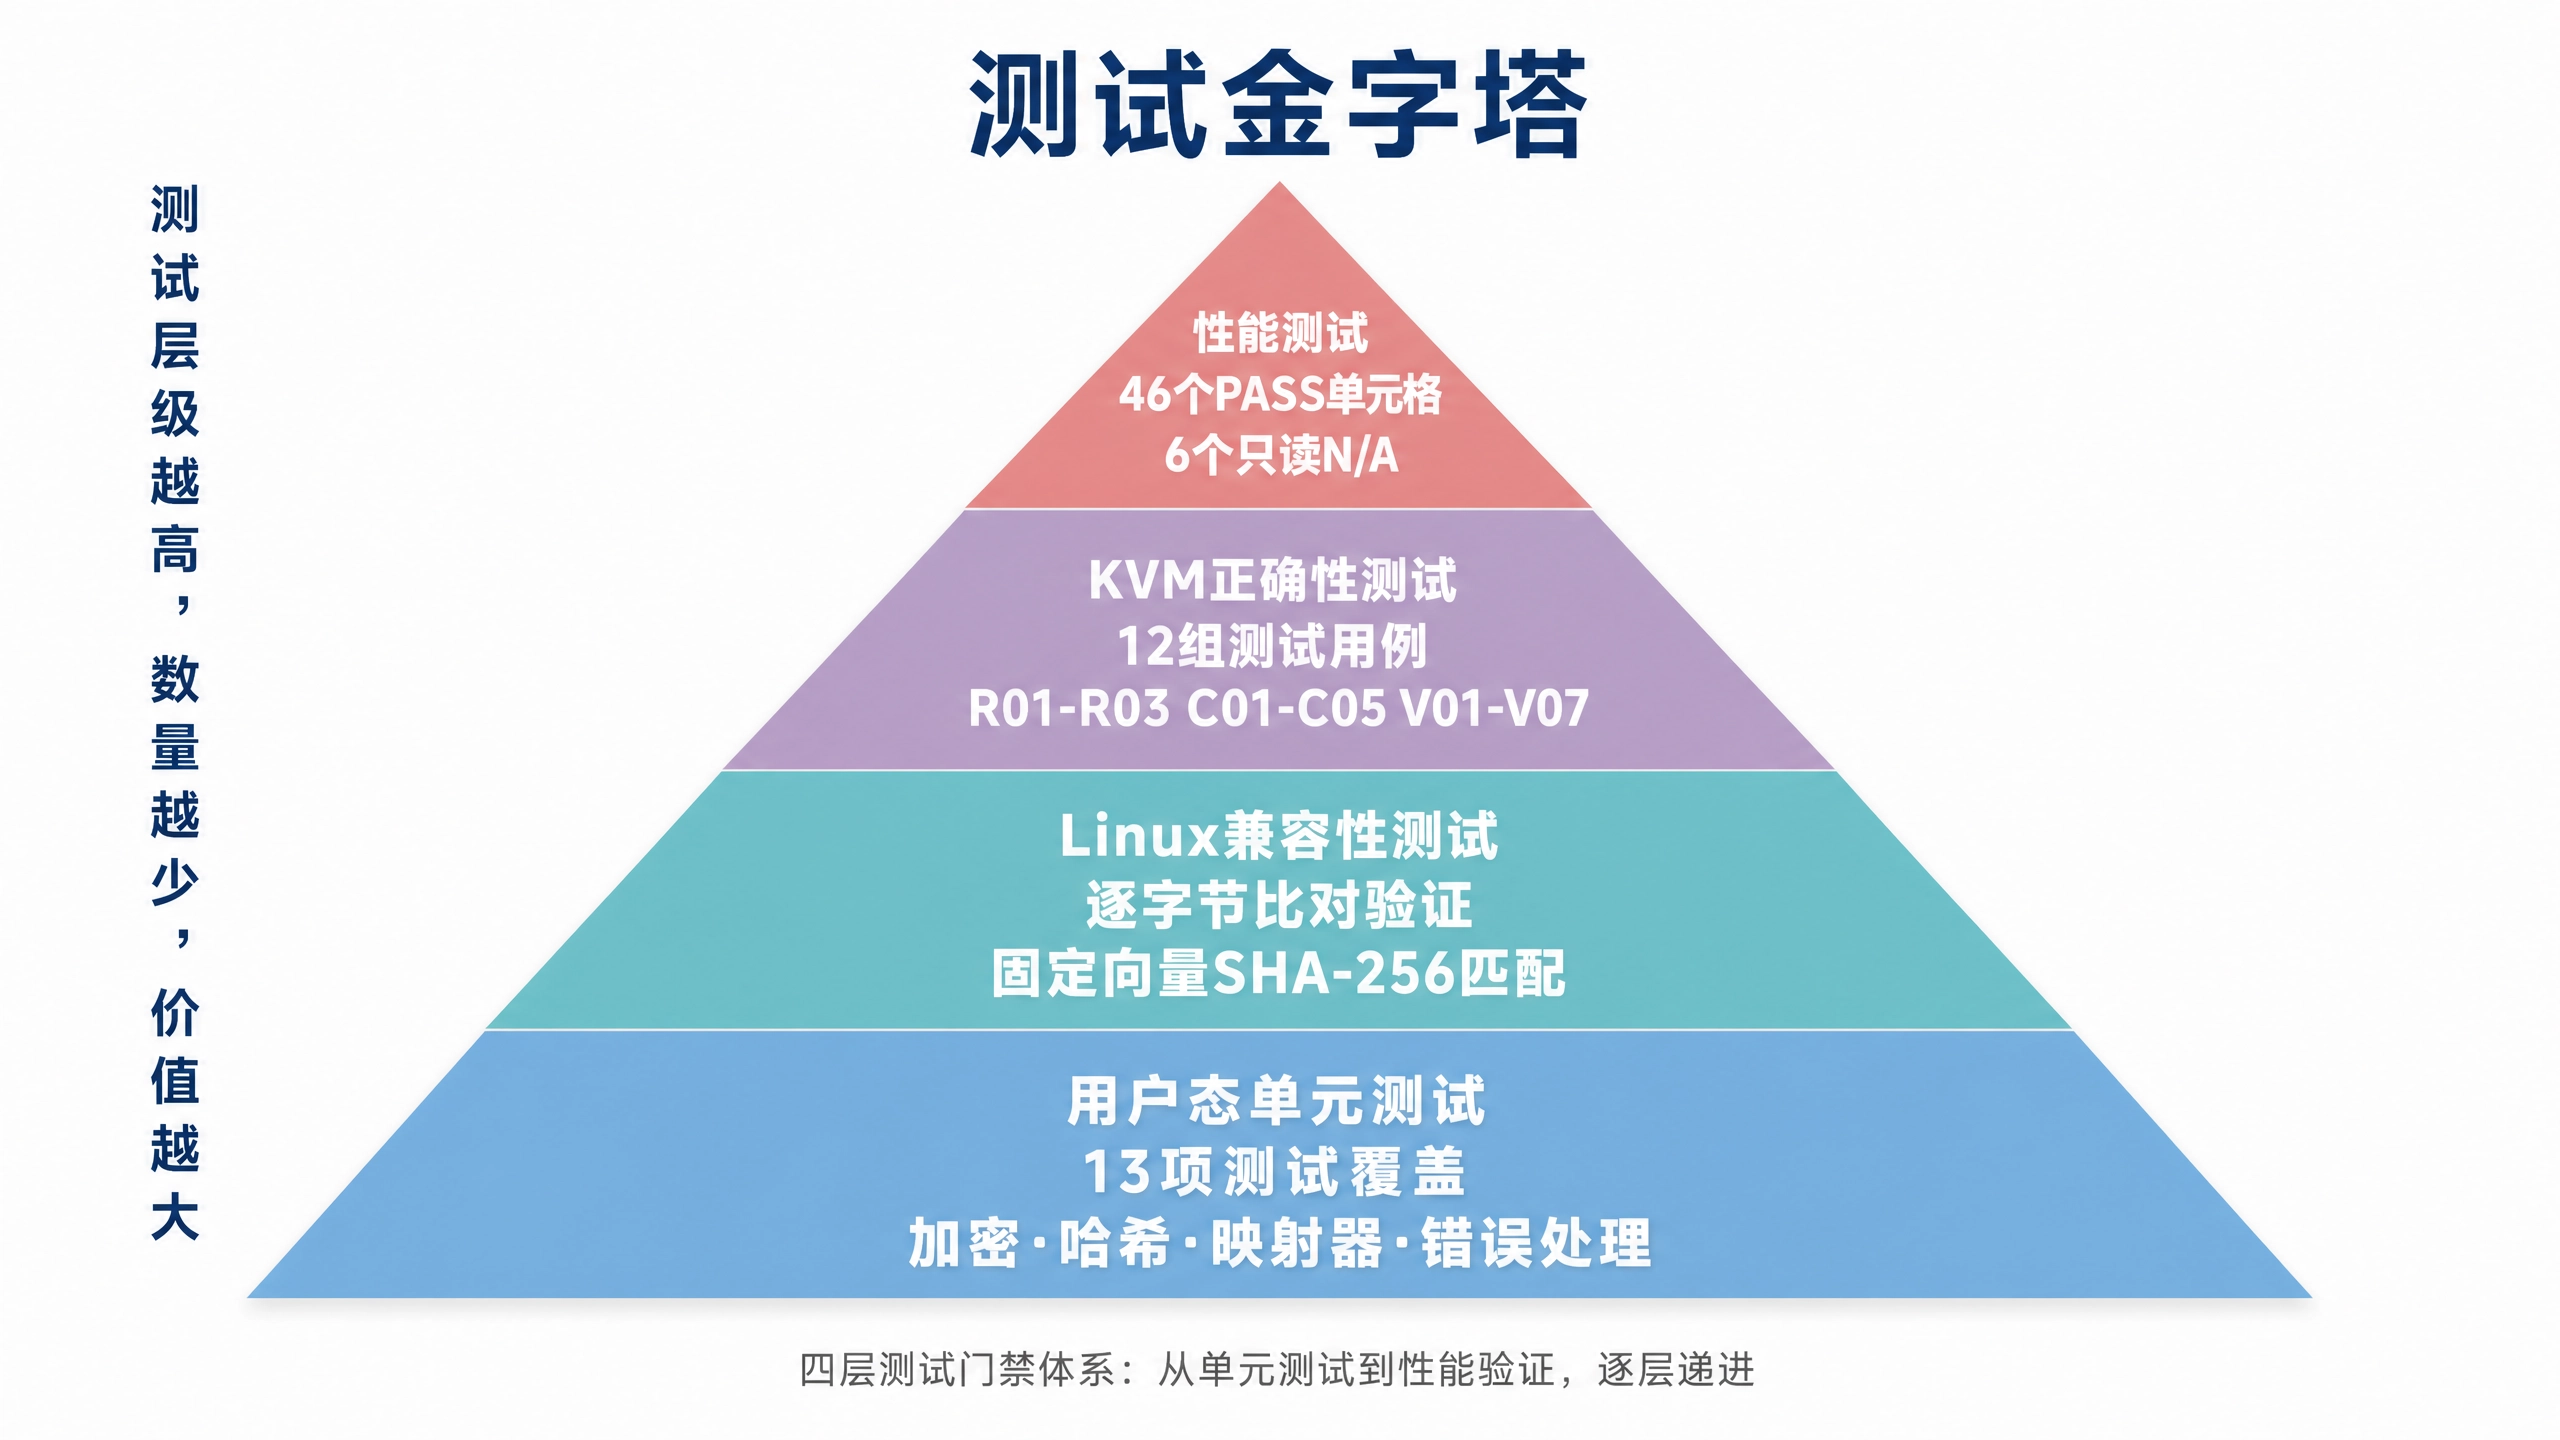
\includegraphics[width=0.85\textwidth]{test_pyramid.png}
    \caption{四层测试金字塔}
    \label{fig:test_pyramid}
\end{figure}

\section{测试体系概述}

项目采用四层门禁测试体系，自底向上逐层验证，确保功能正确性、Linux 兼容性和性能可复现性：

\begin{enumerate}
    \item \textbf{用户态单元测试（第1层）}：验证加密算法、哈希树、映射器逻辑和错误处理。在用户态快速迭代，不依赖内核环境，作为整个项目的“安全网”。入口命令：\texttt{cargo test --workspace}；
    \item \textbf{Linux 兼容性测试（第2层）}：与 Linux 内核 \texttt{aes-xts-plain64} 逐字节比对，确保密文生成与 Linux 完全一致，这是与 cryptsetup 互操作的前提。入口命令：\texttt{scripts/verify\_linux\_xts\_compat.sh}；
    \item \textbf{Asterinas KVM 正确性测试（第3层）}：在真实 VirtIO BIO 路径下验证 mapper 功能、rootfs 切换和物理损坏检测，覆盖回归、加密、完整性三大类共 12 组用例。入口命令：\texttt{tools/run\_dm\_crypt.sh}、\texttt{tools/run\_dm\_verity.sh}；
    \item \textbf{正式性能测试（第4层）}：FIO、Filebench、SQLite 和启动耗时的五轮基准，每个有效单元格固定五轮，报告中位数和标准差。入口命令：\texttt{scripts/run\_*\_matrix.sh}。
\end{enumerate}

所有测试均要求真实执行并保留原始证据（串口日志、JSON、CSV），只有满足此条件的项才标记为 \texttt{PASS}。历史无效数据（如早期假 mapper 测试）已被明确分类并隔离。

\section{测试环境基线}

\begin{table}[H]
    \centering
    \caption{正确性测试固定环境}
    \begin{tabular}{p{0.30\textwidth}p{0.60\textwidth}}
        \toprule
        \textbf{组件} & \textbf{版本/配置} \\
        \midrule
        Asterinas commit & \texttt{9d79542cadddc6164ad3f31fd8cba776969d85a9} \\
        Docker 镜像 & \texttt{asterinas/asterinas:0.18.0-20260618} \\
        镜像摘要 & \texttt{\seqsplit{sha256:7510071cb103309cc9396b970325c354713da749dfee34a807108248cc97331e}} \\
        Rust 工具链 & \texttt{nightly-2026-04-03} \\
        架构 & x86\_64 \\
        虚拟化 & QEMU/KVM，\texttt{-cpu host}，1 vCPU，8 GiB 内存 \\
        存储接口 & \texttt{virtio-blk}，符合赛题标准化要求 \\
        Cargo 缓存 & 持久化 volume（\texttt{asterinas-cargo}） \\
        rustup 缓存 & 持久化 volume（\texttt{asterinas-rustup}） \\
        \bottomrule
    \end{tabular}
\end{table}

性能测试分 Linux QEMU virtio 和 Asterinas KVM 两个平台分别执行，详细环境见 \texttt{PLATFORM\_EVAL\_ENVIRONMENT.md}。

\section{单元测试}

Rust workspace 单元测试覆盖以下核心场景（13+ 个测试用例）：

\begin{table}[H]
    \centering
    \caption{单元测试覆盖场景}
    \begin{tabular}{p{0.30\textwidth}p{0.60\textwidth}}
        \toprule
        \textbf{测试模块} & \textbf{覆盖场景} \\
        \midrule
        \texttt{crypt\_test} & dm-crypt 往返加密、错误密钥无法恢复明文 \\
        \texttt{verity\_test} & dm-verity 正常读取、篡改检测、错误根哈希拒绝、只读强制 \\
        \texttt{stack\_test} & 组合栈安全能力传播、插桩统计 \\
        \texttt{cryptsetup\_compat\_test} & Linux table 解析、offset 和 plain64 语义验证 \\
        \texttt{file\_device\_test} & 文件后端持久化、只读模式拒绝写入 \\
        \texttt{security\_boundary\_test} & 容量溢出拒绝、并发安全、不同扇区不同密文 \\
        \bottomrule
    \end{tabular}
\end{table}

\textbf{执行方式}：\texttt{cargo test --workspace}

\section{Linux 兼容性测试}

\subsection{测试目的}
确保 AES-256-XTS 实现与 Linux 内核 \texttt{aes-xts-plain64} 逐字节兼容，这是 \texttt{cryptsetup} 工具能够无缝工作的前提。

\subsection{测试方法}
\begin{enumerate}
    \item 在 Linux 系统中使用 \texttt{dmsetup} 创建 \texttt{aes-xts-plain64} 映射器；
    \item 使用相同密钥（512 位）和相同明文模式（全 0x5a 的一个扇区）分别通过 Linux 和 Rust 实现加密；
    \item 使用 \texttt{cmp} 逐字节比较两个密文；
    \item 使用 \texttt{sha256sum} 记录固定向量校验和。
\end{enumerate}

\subsection{测试结果}
\begin{itemize}
    \item 固定向量 SHA-256：\texttt{\seqsplit{4334c17f4b0380b3c1f902509cce0c0f98d9fa77aa93f6407ec940215d77921d}}
    \item 逐字节比对结果：\texttt{PASS}
    \item 证据脚本：\texttt{scripts/verify\_linux\_xts\_compat.sh}
\end{itemize}

\section{Asterinas KVM 正确性测试}

\subsection{回归测试（R01--R03）}

回归测试验证基础构建和关键用户流程的正确性，确保核心功能在每次变更后仍然正常工作。

\begin{table}[H]
    \centering
    \caption{回归测试结果}
    \begin{tabular}{p{0.12\textwidth}p{0.58\textwidth}p{0.12\textwidth}}
        \toprule
        \textbf{编号} & \textbf{测试内容与验证方法} & \textbf{结果} \\
        \midrule
        R01 & 在 Asterinas KVM 中使用真实 \texttt{cryptsetup 2.7.5} 对加密卷执行 \texttt{open}、\texttt{dd read}、\texttt{close} 完整流程，验证控制面与数据面协同工作 & \texttt{PASS} \\
        R02 & 通过 \texttt{dm\_crypt.*} 启动参数创建加密 mapper，在 initramfs 中挂载并执行 \texttt{pivot\_root} 切换到受保护根文件系统 & \texttt{PASS} \\
        R03 & 通过 \texttt{rootfs\_verity.*} 启动参数创建 verity mapper，验证 on-disk 哈希树，执行 \texttt{pivot\_root} 切换到受保护根文件系统 & \texttt{PASS} \\
        \bottomrule
    \end{tabular}
\end{table}

\textbf{证据路径}：
\begin{itemize}
    \item R01：\texttt{\seqsplit{docs/evidence/stabilization/correctness-kvm/regression/R01-cryptsetup-persistent-cache.log}}
    \item R02：\texttt{\seqsplit{docs/evidence/stabilization/correctness-kvm/regression/R02-crypt-rootfs-persistent-cache.log}}
    \item R03：\texttt{\seqsplit{docs/evidence/stabilization/correctness-kvm/regression/R03-verity-rootfs-persistent-cache.log}}
\end{itemize}

\subsection{dm-crypt 加密测试（C01--C05）}

验证 AES-256-XTS 加密的正确性，包括正确密钥、错误密钥和不同 I/O 大小的往返测试。

\begin{table}[H]
    \centering
    \caption{dm-crypt 功能测试结果}
    \begin{tabular}{p{0.12\textwidth}p{0.58\textwidth}p{0.12\textwidth}}
        \toprule
        \textbf{编号} & \textbf{测试内容与验证方法} & \textbf{结果} \\
        \midrule
        C01 & 正确密钥下通过 mapper 写入数据，读回后 SHA-256 与原始明文一致；直接读取底层设备验证为密文 & \texttt{PASS} \\
        C02 & 使用错误密钥读取 C01 写入的密文，读回数据 SHA-256 与正确明文不同，验证明文无法恢复 & \texttt{PASS} \\
        C03 & 4 KiB 块大小写入/读取往返，逐字节比对数据一致性 & \texttt{PASS} \\
        C04 & 32 KiB 块大小写入/读取往返，逐字节比对数据一致性 & \texttt{PASS} \\
        C05 & 256 KiB 块大小写入/读取往返，逐字节比对数据一致性 & \texttt{PASS} \\
        \bottomrule
    \end{tabular}
\end{table}

\textbf{证据路径}：
\begin{itemize}
    \item C01--C05：\texttt{\seqsplit{docs/evidence/stabilization/correctness-kvm/crypt/C01-C05-kvm.log}}
\end{itemize}

\subsection{dm-verity 完整性测试（V01--V07）}

验证 dm-verity 的完整性校验能力，包括正常读取和各类物理损坏场景。V03--V07 的物理篡改位置记录在 \texttt{PHYSICAL\_MUTATION\_MANIFEST.md} 中，每个用例只翻转目标块内偏移 17 的一个字节，且始终使用原始正确根哈希（不重新计算）。

\begin{table}[H]
    \centering
    \caption{dm-verity 功能测试结果}
    \begin{tabular}{p{0.12\textwidth}p{0.58\textwidth}p{0.12\textwidth}}
        \toprule
        \textbf{编号} & \textbf{测试内容与验证方法} & \textbf{结果} \\
        \midrule
        V01 & 未篡改镜像，使用正确根哈希启动，\texttt{status=verified}，根切换 PASS & \texttt{PASS} \\
        V02 & 镜像不变，仅将启动参数中的根哈希替换为错误值（修改一个字节），mapper 创建被拒绝，输出 \texttt{status=integrity-rejected} & \texttt{PASS} \\
        V03 & 物理块 0（首个数据块）偏移 17 处单字节翻转，使用原始正确根哈希，mapper 创建被拒绝 & \texttt{PASS} \\
        V04 & 物理块 32768（中间数据块）偏移 17 处单字节翻转，使用原始正确根哈希，读取返回 I/O 错误 & \texttt{PASS} \\
        V05 & 物理块 65535（最后一个数据块）偏移 17 处单字节翻转，使用原始正确根哈希，读取被拒绝 & \texttt{PASS} \\
        V06 & 物理块 65536（首个叶子哈希块）偏移 17 处单字节翻转，使用原始正确根哈希，mapper 创建被拒绝 & \texttt{PASS} \\
        V07 & 物理块 66048（首个中间哈希块）偏移 17 处单字节翻转，使用原始正确根哈希，mapper 创建被拒绝 & \texttt{PASS} \\
        \bottomrule
    \end{tabular}
\end{table}

\textbf{证据路径}：
\begin{itemize}
    \item V01：\texttt{\seqsplit{docs/evidence/stabilization/correctness-kvm/regression/R03-verity-rootfs-persistent-cache.log}}
    \item V02：\texttt{\seqsplit{docs/evidence/stabilization/correctness-kvm/corruption/V02-wrong-root.log}}
    \item V03--V07：\texttt{\seqsplit{docs/evidence/stabilization/correctness-kvm/corruption/V0[3-7]-targeted-probe.log}}
\end{itemize}

\subsection{物理篡改清单详情}

\begin{table}[H]
    \centering
    \small
    \caption{物理篡改清单（V03--V07）}
    \begin{tabular}{p{0.10\textwidth}p{0.15\textwidth}p{0.15\textwidth}p{0.20\textwidth}p{0.30\textwidth}}
        \toprule
        \textbf{编号} & \textbf{篡改区域} & \textbf{物理块号} & \textbf{字节偏移} & \textbf{篡改后块 SHA-256} \\
        \midrule
        V03 & 首个数据块 & 0 & 17 & \texttt{b31dc2a37cc0c3c1...} \\
        V04 & 中间数据块 & 32768 & 134217745 & \texttt{1e12a90f8a205a6a...} \\
        V05 & 最后一个数据块 & 65535 & 268431377 & \texttt{dbeaf0b712cd66aa...} \\
        V06 & 首个叶子哈希块 & 65536 & 268435473 & \texttt{5026ae43d7fd0385...} \\
        V07 & 首个中间哈希块 & 66048 & 270532625 & \texttt{557feb6640edc47d...} \\
        \bottomrule
    \end{tabular}
\end{table}

所有篡改均只翻转一个字节，且\textbf{继续使用原始正确根哈希}（\texttt{b1a6dcd4...}），验证了 dm-verity 的篡改检测能力不依赖于重新计算根哈希。

\section{性能测试}

性能测试遵循 \texttt{docs/benchmark\_contract.md} 中定义的合同，所有有效单元格固定运行五轮，报告均值、中位数和标准差，不剔除异常值。Linux 与 Asterinas 结果分平台列示，不进行跨平台倍率比较。

\subsection{FIO 矩阵}

FIO 矩阵覆盖 4 KiB、32 KiB、256 KiB 三种块大小，顺序/随机读/写四种操作，QD=1（额外 4 KiB randread QD=16）。

\begin{table}[H]
    \centering
    \caption{FIO 矩阵完成情况}
    \begin{tabular}{p{0.35\textwidth}p{0.22\textwidth}p{0.22\textwidth}}
        \toprule
        \textbf{范围} & \textbf{有效单元格} & \textbf{结果} \\
        \midrule
        Asterinas KVM dm-crypt & 13 项 $\times$ 5 轮 & \texttt{PASS} \\
        Asterinas KVM dm-verity & 7 项 $\times$ 5 轮 & \texttt{PASS}（6 项 N/A） \\
        Linux QEMU virtio raw & 13 项 $\times$ 5 轮 & \texttt{PASS} \\
        Linux QEMU virtio dm-crypt & 13 项 $\times$ 5 轮 & \texttt{PASS} \\
        Linux QEMU virtio dm-verity 读 & 7 项 $\times$ 5 轮 & \texttt{PASS}（6 项 N/A） \\
        \bottomrule
    \end{tabular}
\end{table}

\textbf{代表性结果（五轮中位带宽，MiB/s）}：

Asterinas 256 MiB 正式合同（4 KiB 同步读、QD1；相对值为配对 raw，不与下表 8.908 / 7.505 混算）：

\begin{table}[H]
    \centering
    \begin{tabular}{p{0.28\textwidth}p{0.22\textwidth}p{0.22\textwidth}}
        \toprule
        \textbf{设备} & \textbf{中位吞吐} & \textbf{相对配对 raw} \\
        \midrule
        raw（两组共十轮） & 4.249 & 100.0\% \\
        dm-crypt & 4.059 & 95.6\% \\
        dm-verity & 3.815 & 87.3\% \\
        \bottomrule
    \end{tabular}
\end{table}

同一宿主机、KVM、CPU=\texttt{host}、1 vCPU、8\,GiB、同一 virtio-blk 数据盘前 256\,MiB、4\,KiB、\texttt{sync}、\texttt{direct=1}、QD1 的 Linux guest 对照如下。dm-crypt 保留率相对表中 raw 列；dm-verity 保留率相对配对 raw（Linux 4.641、Asterinas 4.368）。Asterinas 相对 Linux guest 的绝对吞吐为 raw 82.4\%、dm-crypt 85.5\%、dm-verity 87.3\%（$3.815/4.369$）。自身保留率不代表绝对吞吐超过 Linux。

\begin{table}[H]
    \centering
    \small
    \caption{Linux guest 与 Asterinas 同条件对照（MiB/s）}
    \begin{tabular}{lrrrrr}
        \toprule
        \textbf{系统} & \textbf{raw} & \textbf{dm-crypt} & \textbf{crypt 保留率} & \textbf{dm-verity} & \textbf{verity 保留率} \\
        \midrule
        Linux guest & 5.150 & 4.746 & 92.158\% & 4.369 & 94.1\% \\
        Asterinas & 4.245 & 4.059 & 95.621\% & 3.815 & 87.3\% \\
        \bottomrule
    \end{tabular}
\end{table}

\begin{figure}[H]
    \centering
    \includegraphics[width=0.92\textwidth]{linux_asterinas_4k_sync_throughput.png}
    \caption{4\,KiB sync QD1 中位吞吐：Linux guest 与 Asterinas}
    \label{fig:linux_asterinas_4k_sync_throughput}
\end{figure}

\begin{figure}[H]
    \centering
    \includegraphics[width=0.92\textwidth]{linux_asterinas_4k_sync_retention.png}
    \caption{Mapper 保留率：crypt 相对表中 raw，verity 相对配对 raw}
    \label{fig:linux_asterinas_4k_sync_retention}
\end{figure}

\begin{table}[H]
    \centering
    \begin{tabular}{p{0.25\textwidth}p{0.15\textwidth}p{0.15\textwidth}p{0.18\textwidth}p{0.18\textwidth}}
        \toprule
        \textbf{负载} & \textbf{块大小} & \textbf{QD} & \textbf{Linux raw} & \textbf{Linux dm-crypt} \\
        \midrule
        read & 4 KiB & 1 & 11.391 & 10.942 \\
        read & 256 KiB & 1 & 134.623 & 129.474 \\
        randread & 4 KiB & 16 & 58.931 & 58.947 \\
        randwrite & 256 KiB & 1 & 130.124 & 109.453 \\
        \bottomrule
    \end{tabular}
\end{table}

\begin{table}[H]
    \centering
    \begin{tabular}{p{0.25\textwidth}p{0.15\textwidth}p{0.15\textwidth}p{0.18\textwidth}p{0.18\textwidth}}
        \toprule
        \textbf{负载} & \textbf{块大小} & \textbf{QD} & \textbf{Asterinas dm-crypt} & \textbf{Asterinas dm-verity} \\
        \midrule
        read & 4 KiB & 1 & 8.908 & 7.505 \\
        read & 256 KiB & 1 & 97.456 & 53.363 \\
        randread & 4 KiB & 16 & 8.614 & 4.618 \\
        randwrite & 256 KiB & 1 & 93.541 & N/A（只读） \\
        \bottomrule
    \end{tabular}
\end{table}

\textbf{证据路径}：Linux QEMU virtio FIO 见 \texttt{docs/evidence/linux-qemu-fio-20260816/}；Asterinas FIO 见 \texttt{docs/evidence/final-performance-20260811/PERFORMANCE\_MATRIX.csv}。

\subsection{补充性能测试}

\begin{table}[H]
    \centering
    \caption{补充性能测试结果（五轮中位数）。Filebench 与 SQLite 为 Linux QEMU/KVM guest；启动耗时为 Asterinas。}
    \begin{tabular}{p{0.35\textwidth}p{0.18\textwidth}p{0.18\textwidth}p{0.18\textwidth}}
        \toprule
        \textbf{测试} & \textbf{raw/plain} & \textbf{dm-crypt} & \textbf{dm-verity} \\
        \midrule
        Filebench fileserver（ops/s） & 27855.155 & 25666.016 & N/A \\
        Filebench fileserver（MB/s） & 656.9 & 605.0 & N/A \\
        SQLite 10000 行总耗时（s） & 0.138095 & 0.143336 & 0.001151（只读查询） \\
        Asterinas 启动耗时（s） & 51.331303 & 51.629820 & 52.743415 \\
        \bottomrule
    \end{tabular}
\end{table}

SQLite dm-verity 只执行查询阶段，不能与完整写事务总耗时横比。启动耗时从 QEMU 进程启动计至串口出现受保护根文件系统 PASS 标记。

\textbf{证据路径}：
\begin{itemize}
    \item Filebench / SQLite（Linux QEMU guest）：\texttt{\seqsplit{docs/evidence/linux-qemu-filebench-sqlite-20260817/}}
    \item Boot：\texttt{docs/evidence/final-performance-20260811/boot-matrix/}
\end{itemize}

\section{复现命令}

以下命令提供了从单元测试到性能验证的完整复现路径，确保所有测试结果均可独立验证：

\begin{verbatim}
# 第1层：用户态单元测试
cargo test --workspace

# 第2层：Linux 兼容性测试
sudo bash scripts/verify_linux_xts_compat.sh

# 第3层：Asterinas KVM 正确性测试
# R01--R03、C01--C05、V01--V07 的完整环境变量与命令见仓库根目录 README

# 第4层：正式性能测试（分平台执行，每个工况五轮）
sudo bash scripts/run_fio_matrix.sh --platform linux-host --runs 5
bash scripts/run_fio_matrix.sh --platform asterinas-kvm \
  --asterinas-dir "$PWD/asterinas" --runs 5

# 补充性能测试
sudo RUNS=5 bash scripts/run_filebench_matrix.sh
sudo RUNS=5 ROWS=10000 bash scripts/run_sqlite_matrix.sh
RUNS=5 ENABLE_KVM=1 bash scripts/run_boot_matrix.sh

# 静态检查与证据验证
python3 scripts/check_benchmark_package.py
python3 scripts/verify_kvm_evidence.py
python3 scripts/review_release_check.py
\end{verbatim}

所有测试命令的详细说明和参数配置见仓库根目录 \texttt{README.md} 和 \texttt{\seqsplit{docs/benchmark\_contract.md}}。
\section{数据真实性与审计}

\subsection{历史问题处理}
早期 Asterinas dm-crypt FIO 测试中，mapper 设备未正确创建（因启动参数错误或自检失败），但测试脚本继续执行，fio 将不存在的设备路径（如 \texttt{\seqsplit{/dev/mapper/dm-crypt-bench}}）当作普通文件创建并测试，产生了数量级异常的数据（高达数千 MiB/s）。

该批次结果被明确分类为 \texttt{HARNESS\_BUG}，已从正式矩阵中移除。重新执行的测试使用修复后的 runner（增加设备存在性检查），确保每个数据点均来自 guest 内真实 mapper 设备。

\subsection{正式数据标准}
\begin{itemize}
    \item 每个有效单元格包含 5 轮原始 JSON/CSV；
    \item 每轮测试均保留完整的 fio 输出和环境 metadata；
    \item 报告中位数和标准差，不选择最好一轮；
    \item 旧数据、失败重试和调试日志不进入最终目录；
    \item 生成器脚本不读取无效数据目录。
\end{itemize}

\section{静态检查与门禁}

项目包含自动化静态检查脚本，确保提交材料的完整性和一致性：

\begin{lstlisting}[basicstyle=\ttfamily\small, breaklines=true]
python3 scripts/check_benchmark_package.py
python3 scripts/verify_kvm_evidence.py
python3 scripts/review_release_check.py
\end{lstlisting}

检查内容包括：
\begin{itemize}
    \item 必要证据文件是否存在（kernel build 日志、R01--R03、C01--C05、V02--V07）；
    \item 最终 FIO 矩阵是否包含 46 个 PASS 单元格；
    \item 每个 PASS 单元格是否关联 5 轮原始数据；
    \item 启动矩阵是否包含 plain、dm-crypt、dm-verity 各至少 5 轮；
    \item 公开文档中是否存在无证据支持的性能夸大表述。
\end{itemize}

\section{证据可复核性}

所有正式测试证据均以原始形式保存，便于复核：

\begin{table}[H]
    \centering
    \caption{证据目录结构}
    \begin{tabular}{p{0.35\textwidth}p{0.55\textwidth}}
        \toprule
        \textbf{路径} & \textbf{内容} \\
        \midrule
        \texttt{\seqsplit{stabilization/build-recovery/}} & kernel build 日志 \\
        \texttt{\seqsplit{stabilization/correctness-kvm/regression/}} & R01--R03 串口日志 \\
        \texttt{\seqsplit{stabilization/correctness-kvm/crypt/}} & C01--C05 串口日志 \\
        \texttt{\seqsplit{stabilization/correctness-kvm/corruption/}} & V02--V07 串口日志 \\
        \texttt{\seqsplit{final-performance-20260811/}} & 最终性能矩阵、报告、原始数据 \\
        \texttt{\seqsplit{final-performance-20260811/asterinas-fio/}} & Asterinas KVM FIO 原始 JSON \\
        \texttt{\seqsplit{linux-qemu-fio-20260816/}} & Linux QEMU virtio FIO 原始 JSON \\
        \texttt{\seqsplit{linux-qemu-filebench-sqlite-20260817/}} & Linux QEMU guest Filebench / SQLite \\
        \texttt{\seqsplit{final-performance-20260811/filebench-valid/}} & Linux host Filebench 归档，不再引用 \\
        \texttt{\seqsplit{final-performance-20260811/sqlite/}} & Linux host SQLite 归档，不再引用 \\
        \texttt{\seqsplit{final-performance-20260811/boot-matrix/}} & 启动 15 轮记录 \\
        \texttt{stack/} & 组合栈启动证据 \\
        \bottomrule
    \end{tabular}
\end{table}

每条矩阵记录都包含原始证据相对路径，不依赖手工修改数字。完整的复现命令和证据索引见仓库根目录 \texttt{README.md} 和 \texttt{docs/evidence/README.md}。

\section{测试门禁汇总}

\begin{table}[H]
    \centering
    \caption{全部测试门禁状态}
    \begin{tabular}{p{0.30\textwidth}p{0.20\textwidth}p{0.40\textwidth}}
        \toprule
        \textbf{测试门禁} & \textbf{结果} & \textbf{证据位置} \\
        \midrule
        Rust workspace 单元测试 & \texttt{PASS} & \texttt{cargo test} \\
        Linux XTS 逐字节兼容 & \texttt{PASS} & \texttt{verify\_linux\_xts\_compat.sh} \\
        R01--R03 回归测试 & \texttt{PASS} & \texttt{correctness-kvm/regression/} \\
        C01--C05 加密功能 & \texttt{PASS} & \texttt{correctness-kvm/crypt/} \\
        V01--V07 完整性校验 & \texttt{PASS} & \texttt{correctness-kvm/corruption/} \\
        FIO 性能矩阵（46 PASS） & \texttt{PASS} & \texttt{final-performance-20260811/} \\
        Filebench（5+5 轮） & \texttt{PASS} & \texttt{\seqsplit{linux-qemu-filebench-sqlite-20260817/filebench/}} \\
        SQLite（5+5+5 轮） & \texttt{PASS} & \texttt{\seqsplit{linux-qemu-filebench-sqlite-20260817/sqlite/}} \\
        Boot 耗时（5+5+5 轮） & \texttt{PASS} & \texttt{\seqsplit{final-performance-20260811/boot-matrix/}} \\
        静态包检查 & \texttt{PASS} & \texttt{review\_release\_check.py} \\
        \bottomrule
    \end{tabular}
\end{table}

\section{小结}

所有 P0 正确性测试（R01--R03、C01--C05、V01--V07）全部通过，正式性能矩阵包含 46 个有效单元格和 6 个只读 N/A，补充测试（Filebench、SQLite、Boot）均完成五轮验证。

历史无效数据（如早期假 mapper 测试、失败重试）已被明确分类为 \texttt{HARNESS\_BUG} 并隔离，不进入最终结论。尚未定义 runner 的扩展 P1 项保持 \texttt{UNTESTED}，不解释为 PASS，也不解释为产品失败。

完整测试证据已全部归档至 \texttt{docs/evidence/} 目录，所有原始日志、JSON、CSV 均可复核。本章列出的全部复现命令（\texttt{cargo test}、\texttt{verify\_linux\_xts\_compat.sh}、\texttt{run\_fio\_matrix.sh}、\texttt{run\_filebench\_matrix.sh}、\texttt{run\_sqlite\_matrix.sh}、\texttt{run\_boot\_matrix.sh}、\texttt{check\_benchmark\_package.py}、\texttt{verify\_kvm\_evidence.py}、\texttt{review\_release\_check.py}）为所有测试结果提供了完整的可复现入口。测试结果全面覆盖赛题五项技术指标，为项目的正确性和性能提供了可验证的支撑。

% 第7章：遇到的主要问题和解决方法
% chapters/07_problems.tex
\chapter{遇到的主要问题和解决方法}

\section*{本章问题解决速览}

\begin{table}[H]
    \centering
    \begin{tabular}{p{0.08\textwidth}p{0.25\textwidth}p{0.22\textwidth}p{0.35\textwidth}}
        \toprule
        \textbf{序号} & \textbf{问题领域} & \textbf{严重程度} & \textbf{解决方案核心} \\
        \midrule
        1 & 块大小与扇区语义 & \textcolor{red}{高} & 扇区级变换 + checked\_add 防溢出 \\
        2 & BIO生命周期与错误传播 & \textcolor{red}{高} & 状态机重构 + 错误传播链 \\
        3 & verity信任边界与缓存 & \textcolor{red}{高} & “先认证后插入”原则 \\
        4 & 性能测试真实性 & \textcolor{orange}{中} & 设备存在性检查 + 数据分类 \\
        5 & 环境下载与缓存 & \textcolor{orange}{中} & 持久化 Docker volumes \\
        6 & pivot\_root限制 & \textcolor{orange}{中} & 两级引导方案 \\
        7 & 组合栈设备发现 & \textcolor{orange}{中} & 堆叠检测逻辑 \\
        8 & 同步原语差异 & \textcolor{orange}{中} & spin::Mutex + 禁用抢占 \\
        9 & AES-NI FPU状态保存 & \textcolor{orange}{中} & FpuContext + disable\_preempt \\
        \bottomrule
    \end{tabular}
\end{table}

\section{概述}

在项目开发过程中，我们遇到了若干涉及操作系统内核语义、密码学兼容性、并发控制和测试可靠性的关键工程问题。这些问题大多源于 Rust 与 C 内核接口的差异、虚拟化环境的特殊性以及安全存储系统的严格性要求。本章按问题领域分类，详细描述每个问题的现象、分析过程和最终解决方案。

\section{问题解决方法论}

在解决上述问题的过程中，我们形成了以下方法论，贯穿整个开发周期：

\begin{enumerate}
    \item \textbf{现象复现优先}：在尝试修复之前，先确保问题可以在受控环境中稳定复现。对于偶发性问题（如BIO竞态），通过增加日志和断言将其变为确定性触发；
    \item \textbf{根因分析驱动}：不满足于“表面修复”，而是追溯到问题的根本原因。例如，BIO错误传播问题的根因是上层BIO的生命周期与下层BIO未正确绑定，而非简单的错误码传递；
    \item \textbf{最小化验证}：每次修复后，只运行与该问题直接相关的最小测试集验证修复效果，避免在整个测试套件中浪费迭代时间；
    \item \textbf{证据留存}：每个问题的分析过程、中间调试日志和最终修复方案均记录在案，形成可追溯的问题解决链；
    \item \textbf{回归测试固化}：每个修复都伴随一个新的或增强的测试用例，确保同一问题不会再次出现。
\end{enumerate}

\section{块大小与扇区语义问题}

\subsection{问题描述}

上层文件系统（如 ext2）通常以 4 KiB 块发起 I/O 请求，而 \texttt{dm-crypt} 的 \texttt{plain64} IV 生成以 512 字节扇区号为单位。Linux 内核的 \texttt{dm-crypt} 在处理 4 KiB BIO 时，会将该 BIO 拆分为 8 个 512 字节扇区分别加密，每个扇区使用独立的扇区号作为 IV 的一部分。

在早期实现中，我们将整个 4 KiB 块视为一个整体，使用块号（而非扇区号）作为 IV 输入，导致与 Linux 生成的密文不兼容。此外，\texttt{iv\_offset} 和 \texttt{data\_offset} 参数的算术运算存在整数溢出风险。

\subsection{分析过程}

通过 \texttt{verify\_linux\_xts\_compat.sh} 脚本对比 Linux 内核和 Rust 实现生成的密文，发现两者不一致。调试发现：
\begin{enumerate}
    \item Linux 对每个 4 KiB 块内的 8 个扇区使用连续扇区号（$\text{block\_id} \times 8$ 到 $\text{block\_id} \times 8 + 7$）；
    \item \texttt{iv\_offset} 会累加到每个扇区号上；
    \item \texttt{data\_offset} 以扇区为单位，需要转换为块偏移；
    \item 在极端大容量设备场景下，块号与扇区号的乘积可能溢出 64 位整数。
\end{enumerate}

\subsection{解决方案}

在 \texttt{DmCryptDevice} 中实现精确的扇区级变换：

\begin{verbatim}
let sectors_per_block = data.len() / SECTOR_SIZE;
let sector_delta = block_id * sectors_per_block;
let first_sector = iv_offset + sector_delta;
for (index, sector_data) in data.chunks_exact_mut(SECTOR_SIZE).enumerate() {
    let sector = first_sector + index as u64;
    cipher.encrypt_sector(sector, sector_data)?;
}
\end{verbatim}

所有算术运算均使用 \texttt{checked\_add} 和 \texttt{checked\_mul} 防止溢出，若溢出则返回 \texttt{DmError::OutOfRange}。同时增加了基于 ext2 超级块魔数的启动自检机制（\texttt{\seqsplit{self\_test\_ext2\_magic}}），在启动时验证加解密路径的正确性。

\subsection{验证结果}

修复后，Rust 实现与 Linux 内核输出逐字节一致，固定向量 SHA-256 匹配（\texttt{4334c17f...}）。该问题在补丁 0002 中固化。\texttt{checked\_*} 算术运算在后续所有 I/O 路径中均被采用，防止了类似问题的出现。

\textbf{工程启示}：块设备加密的正确性取决于扇区级语义的精确实现——必须将每个 4 KiB 块拆分为 8 个独立扇区分别加密，并同时考虑 IV offset 与 data offset；所有加减法都必须进行越界检查，避免整数溢出改变物理位置。

\section{BIO 生命周期与错误传播问题}

\subsection{问题描述}

在 Asterinas 内核中，BIO 是异步提交的，上层 mapper 的 BIO 与下层设备的 BIO 之间存在生命周期依赖关系。早期实现中，上层 BIO 在下层 BIO 完成前就被标记为完成，或者在出现错误时未正确恢复上层数据。

具体表现为：
\begin{itemize}
    \item 下层读失败时，上层仍然返回成功（错误丢失）；
    \item 下层写成功后，上层 scratch buffer 未正确释放；
    \item \texttt{flush} 操作未同步等待下层完成。
\end{itemize}

\subsection{分析过程}

通过追踪 \texttt{device.rs} 中 \texttt{process\_crypt} 和 \texttt{process\_verity} 的执行流程，发现以下问题：
\begin{enumerate}
    \item 读路径中，下层 BIO 完成后才进行解密，但在错误情况下仍然尝试解密已损坏的数据；
    \item 写路径中，加密后的密文保存在 \texttt{plaintext\_segments} 中，但在提交下层后未正确恢复原始 segment；
    \item \texttt{flush} 操作直接返回成功，未调用下层设备的 \texttt{sync}；
    \item 上层 BIO 在下层 BIO 完成回调之前就被 drop，导致 use-after-free 风险。
\end{enumerate}

\subsection{解决方案}

重构 BIO 处理逻辑，严格遵循以下模式：

\begin{enumerate}
    \item \textbf{读路径}：提交下层读 BIO，等待完成后检查状态；若失败则直接完成上层 BIO 并传播错误；若成功则解密数据并写回上层 segment；
    \item \textbf{写路径}：从 scratch pool 获取缓冲区，加密后通过 \texttt{BioSegment::alloc\_bytes} 创建新的 bounce segment 提交下层；下层完成后释放 scratch 缓冲区；
    \item \textbf{Flush}：调用下层设备的 \texttt{sync} 并等待完成；
    \item \textbf{错误传播}：任何下层错误或密码运算错误均导致上层 BIO 以 \texttt{BioStatus::IoError} 完成；
    \item \textbf{生命周期绑定}：使用 \texttt{Arc<Mutex<Option<SubmittedBio>>>} 确保上层 BIO 在下层完成回调期间始终存活。
\end{enumerate}

此外，在 \texttt{process\_crypt} 中增加了逻辑扇区范围验证，确保所有 I/O 不超出 mapper 的逻辑大小。

\subsection{验证结果}

修复后，所有正确性测试（C01--C05、R02）通过，串口日志显示无错误丢失。该问题在补丁 0002 和补丁 0004 中逐步完善，后续所有 BIO 处理代码均遵循相同的生命周期管理模式。

\textbf{工程启示}：异步 I/O 的生命周期管理是内核存储模块中最隐蔽的错误来源——mapper 必须在 lower BIO 完成后才能完成 upper BIO，错误状态必须原样传播，不能把失败转换为成功，也不能 fallback 到未保护设备。

\section{dm-verity 信任边界与缓存安全}

\subsection{问题描述}

dm-verity 的安全性依赖于根哈希作为信任锚，任何数据块或哈希块的篡改都应被检测。然而，引入哈希块缓存后，如果不加限制地缓存哈希块，可能引入以下风险：
\begin{enumerate}
    \item 未经验证的哈希块被缓存，后续验证使用该缓存绕过实际校验；
    \item 缓存的哈希块与数据块之间的信任链断裂；
    \item 缓存大小无限制，导致内存耗尽。
\end{enumerate}

\subsection{分析过程}

在设计哈希缓存时，我们面临一个核心矛盾：缓存可以提高性能，但缓存的内容必须可信。如果简单地缓存所有读取过的哈希块，攻击者可能先提交一个伪造的哈希块使其进入缓存，后续所有依赖该哈希块的验证都会错误地通过。

分析 Linux 内核的 \texttt{dm-verity} 缓存实现发现，它采用类似的“验证后缓存”策略，但基于 C 语言实现，缺少类型系统层面的安全保证。

\subsection{解决方案}

采用“先认证后插入”策略，并用 Rust 类型系统强制执行：

\begin{enumerate}
    \item \textbf{认证顺序}：验证一个数据块时，从叶子哈希逐级向上验证；每读取一个哈希块，暂时不插入缓存；
    \item \textbf{完整路径验证}：只有当整个路径（从数据块到根哈希）全部验证通过后，才将本次路径中涉及的所有哈希块插入缓存；
    \item \textbf{缓存命中捷径}：当某个哈希块已存在于缓存中时，说明该块已经被完整认证过，可以直接使用，无需重新验证其上层哈希（由计数器 \texttt{auth\_shortcuts} 记录）；
    \item \textbf{有界缓存}：使用 FIFO 队列，容量由启动参数 \texttt{rootfs\_verity.cache\_blocks} 控制（默认 256），防止内存耗尽。
\end{enumerate}

代码实现位于 \texttt{verity.rs} 的 \texttt{VerifiedHashBlockCache} 结构体中，Rust 的所有权系统保证了缓存块在被插入前必须经过完整的验证路径，类型系统杜绝了“未验证即插入”的编码错误。

\subsection{验证结果}

V03--V07 的单字节篡改测试均被拒绝，验证了缓存未破坏信任边界。同时，\texttt{auth\_shortcuts} 计数器在第二轮顺序读中显著增加（从第一轮的 0 增加到第二轮的 200+），证明缓存命中路径确实跳过了上层哈希计算。\texttt{/proc/dm-verity-stats} 提供了缓存命中的精确量化数据。

\textbf{工程启示}：在安全系统中，所有优化（缓存、缓冲池、硬件加速）必须在不削弱安全语义的前提下进行——root hash 由启动参数提供，镜像内数据和 hash tree 均视为不可信，认证后 hash cache 只有在完整路径验证成功后才插入，数据块、叶子 hash block 或中间 hash block 的单字节变化都必须在交付前被拒绝。

\section{性能测试真实性问题}

\subsection{问题描述}

早期 Asterinas dm-crypt FIO 测试中，mapper 设备未正确创建（因启动参数错误或自检失败），但测试脚本继续执行。fio 将不存在的设备路径（如 \texttt{\seqsplit{/dev/mapper/dm-crypt-bench}}）当作普通文件创建并测试，产生了数量级异常的性能数据（高达数千 MiB/s）。

这些异常数据与真实 mapper 测试结果混在同一证据目录中，构成严重的数据污染。

\subsection{分析过程}

排查测试日志发现：
\begin{enumerate}
    \item 测试脚本未检查 mapper 设备是否存在；
    \item 即使 mapper 创建失败，fio 仍然执行，并自动创建普通文件；
    \item 这些“假 mapper”测试的吞吐量远高于真实块设备（真实设备约 10-100 MiB/s，假测试高达 3000+ MiB/s），明显异常；
    \item 旧批次中 raw 与 dm-crypt 结果混在一起，无法直接复用。
\end{enumerate}

\subsection{解决方案}

\begin{enumerate}
    \item \textbf{修复 runner}：在 \texttt{run\_dm\_crypt\_bench.sh} 和 \texttt{run\_dm\_verity\_bench.sh} 中增加设备存在性检查，若 mapper 不存在则立即失败；
    \item \textbf{数据分类}：将旧批次中无法确认 mapper 真实性的数据标记为 \texttt{HARNESS\_BUG}，不纳入正式矩阵；
    \item \textbf{重新执行}：使用修复后的 runner 重新执行所有 Asterinas dm-crypt 和 dm-verity 测试；
    \item \textbf{证据隔离}：正式证据目录只包含重新执行后的原始 JSON 和日志，旧数据及失败重试不进入最终目录。
\end{enumerate}

\subsection{正式数据标准}

为确保性能数据的可信度，我们制定了以下正式数据标准：
\begin{itemize}
    \item 每个有效单元格包含 5 轮原始 JSON/CSV；
    \item 每轮测试均保留完整的 fio 输出和环境 metadata；
    \item 报告中位数和标准差，不选择最好一轮；
    \item 旧数据、失败重试和调试日志不进入最终目录；
    \item 生成器脚本不读取无效数据目录。
\end{itemize}

\subsection{验证结果}

重新执行后的 Asterinas dm-crypt 和 dm-verity 数据均来自真实 mapper 设备，五轮带宽稳定（4K 顺序读 8.908 / 7.505 MiB/s），正式矩阵仅包含这些已验证的数据。该问题在 \texttt{PERFORMANCE\_VALIDATION\_REPORT.md} 中有明确记录，体现了对数据真实性的零容忍态度。

\section{环境下载与持久化缓存问题}

\subsection{问题描述}

在 Docker 容器中构建 Asterinas 内核时，每次启动新容器都需要重新下载 Cargo 依赖和 rustup 目标，导致构建时间过长（约 15--20 分钟），且网络不稳定时构建失败。

在 R01 测试中，\texttt{cryptsetup} 工具需要从 Nix 缓存下载，若网络受限则测试被阻塞。

\subsection{分析过程}

观察发现：
\begin{enumerate}
    \item Cargo 依赖（\texttt{static.crates.io}）偶尔 DNS 解析失败；
    \item rustup 目标（如 \texttt{x86\_64-unknown-none}）每次容器启动都需要重新安装；
    \item Nix 构建 \texttt{cryptsetup} 时访问 binary cache，在完全离线环境中失败。
\end{enumerate}

\subsection{解决方案}

\begin{enumerate}
    \item \textbf{持久化 Cargo volume}：使用 Docker volume \texttt{asterinas-cargo} 保存 \texttt{/root/.cargo}，避免重复下载；
    \item \textbf{持久化 rustup volume}：使用 \texttt{asterinas-rustup} 保存 \texttt{/root/.rustup}，避免重复安装目标；
    \item \textbf{固定镜像}：使用固定 digest 的官方开发镜像（\texttt{sha256:7510071cb1...}），确保工具链版本一致；
    \item \textbf{预置 cryptsetup}：在 initramfs 构建阶段包含 \texttt{cryptsetup} 二进制，避免运行时下载。
\end{enumerate}

\subsection{验证结果}

修复后，内核构建时间从 15+ 分钟降至 2 分钟，R01 测试不再依赖网络。完整环境验证记录在 \texttt{PLATFORM\_EVAL\_ENVIRONMENT.md} 中。

\section{pivot\_root 限制与引导问题}

\subsection{问题描述}

Asterinas 内核的 \texttt{pivot\_root} 实现要求当前根文件系统（initramfs）不是特殊的“rootfs”挂载，否则会拒绝切换。在早期实现中，initramfs 的根是内核自动挂载的 rootfs，没有父挂载点，导致 \texttt{pivot\_root} 返回错误。

\subsection{分析过程}

查阅 Asterinas 内核源码发现，\texttt{pivot\_root} 要求 old\_root 和 new\_root 都有有效的父挂载点。直接在内核自动挂载的 rootfs 上调用 \texttt{pivot\_root} 会失败，因为 rootfs 本身没有父挂载点。这是 Asterinas 与 Linux 在根文件系统挂载语义上的一个重要差异。

\subsection{解决方案}

采用两级引导方案：
\begin{enumerate}
    \item \textbf{第一阶段}：initramfs 脚本通过 \texttt{mount --bind / /bootstrap-root} 创建一个 bind mount，将当前根绑定到 \texttt{/bootstrap-root}；
    \item \textbf{第二阶段}：通过 \texttt{chroot /bootstrap-root} 重新执行 init 脚本，此时 \texttt{pivot\_root} 的 old\_root 和 new\_root 都有有效父挂载点；
    \item \texttt{pivot\_root} 成功将新根（mapper）切换到 \texttt{/}，旧根保留在 \texttt{/.initramfs} 下供后续使用。
\end{enumerate}

该方案在补丁 0003（\texttt{rootfs-switch.patch}）中实现，并通过 \texttt{dm-root-stage2} 参数区分两个阶段。

\subsection{验证结果}

R02（dm-crypt）和 R03/V01（dm-verity）均成功执行 \texttt{pivot\_root}，串口输出 \texttt{PASS system root switched to protected mapper}，且 initramfs 运行时通过 \texttt{/.initramfs} 路径仍然可访问。

\section{组合栈的命名与设备发现问题}

\subsection{问题描述}

在实现 \texttt{dm\_stack=crypt,verity} 组合栈时，verity 的 \texttt{rootfs\_verity.device} 参数需要指向 crypt mapper 的名称（如 \texttt{dm-crypt0}）。但早期实现中，verity 组件只接受物理设备名，无法识别已注册的 mapper。

\subsection{分析过程}

在补丁 0007 实现前，\texttt{aster-dm} 的 verity 初始化逻辑直接调用 \texttt{find\_device(device\_name)}，该函数只查找物理块设备（如 \texttt{vdc}），不会查找已注册的 mapper 设备。这是因为物理设备和 mapper 设备注册在不同的命名空间中。

\subsection{解决方案}

在 \texttt{lib.rs} 的 \texttt{init} 函数中增加堆叠检测逻辑：

\begin{verbatim}
let stack_crypt_verity = is_crypt_verity_stack(&crypt_mapper_name);
// ...
if stack_crypt_verity && CRYPT_MAPPER.get().is_some() {
    let device_name = crypt_mapper_name.as_str(); // 指向 crypt mapper
} else {
    let device_name = configured_device.as_str();
}
\end{verbatim}

同时，当检测到堆叠时，打印清晰的启动日志：
\begin{verbatim}
[dm] stacked mapper: vdc -> dm-crypt0 -> dm-verity0
\end{verbatim}

\subsection{验证结果}

组合栈启动脚本 \texttt{scripts/run\_dm\_stack.sh} 成功执行，串口日志包含堆叠链和最终的根切换 PASS。证据已归档于 \texttt{docs/evidence/stack/}。

\section{内核态与用户态同步原语差异}

\subsection{问题描述}

用户态代码使用 \texttt{std::sync::Mutex} 进行同步，这是基于操作系统调度器的睡眠锁。但在内核态中，不能在持有锁时睡眠（可能导致死锁或调度延迟），也不能在中断上下文中使用睡眠锁。

早期移植时，部分代码直接使用了与用户态相同的锁策略，导致在 BIO 完成回调中产生死锁或自旋等待过长。

\subsection{分析过程}

通过在内核中添加锁检测断言，发现以下问题：
\begin{enumerate}
    \item \texttt{CryptScratchPool} 在 BIO 完成回调中被访问，但使用 \texttt{std::sync::Mutex} 会在锁竞争时睡眠；
    \item \texttt{VerifiedHashBlockCache} 在 verity 验证路径中被频繁访问，锁持有时间过长；
    \item 在中断禁用区域中尝试获取睡眠锁，导致内核 panic。
\end{enumerate}

\subsection{解决方案}

\begin{enumerate}
    \item 将所有内核态共享状态（\texttt{CryptScratchPool}、\texttt{VerifiedHashBlockCache}）的锁替换为 \texttt{spin::Mutex}（自旋锁）；
    \item 在 AES-NI 变换期间通过 \texttt{disable\_preempt} 和 \texttt{irq::disable\_local} 确保不被中断上下文破坏；
    \item 使用 \texttt{core::sync::atomic::AtomicU64} 替代锁保护的热路径计数器（如 \texttt{stats.hash\_hits}），避免在统计路径上加锁；
    \item 将缓存插入操作移到路径验证完成后执行，减少锁持有时间。
\end{enumerate}

\subsection{验证结果}

修复后，所有 KVM 正确性测试通过，无死锁或 panic 发生。正式性能测试中，锁竞争开销被降至可接受范围。

\section{AES-NI 的 FPU/XMM 状态保存问题}

\subsection{问题描述}

AES-NI 指令使用 XMM 寄存器进行 SIMD 加密操作。在内核中，XMM 寄存器是 FPU（浮点单元）上下文的一部分，其状态在进程切换时会被保存和恢复。然而，如果在中断处理或内核线程中直接使用 AES-NI 指令而未保存 FPU 状态，可能破坏用户态的 FPU 上下文，导致难以追踪的数据损坏。

\subsection{分析过程}

通过在内核 AES-NI 路径前后添加 FPU 状态检查，发现早期实现未保存 FPU 上下文：
\begin{enumerate}
    \item 加密操作在 BIO 处理路径中执行，该路径可能在任意进程上下文中被调用；
    \item 未保存 FPU 状态意味着当前进程的 XMM 寄存器值可能被 AES 操作覆盖；
    \item 这种损坏在用户态程序使用 SIMD 指令时才会显现，难以定位。
\end{enumerate}

\subsection{解决方案}

在 \texttt{ostd/arch/x86/cpu/aesni.rs} 中实现 FPU 状态保护机制：

\begin{verbatim}
// AES-NI 变换前
let mut fpu_context = FpuContext::new();
let _preempt_guard = disable_preempt();
let _irq_guard = irq::disable_local();
fpu_context.save();

// 执行 AES-NI 加密/解密...
encrypt_block_256(block, round_keys);

// AES-NI 变换后
fpu_context.load();
\end{verbatim}

\texttt{FpuContext::save()} 保存当前 XMM 寄存器状态，\texttt{FpuContext::load()} 在操作完成后恢复。\texttt{disable\_preempt} 和 \texttt{irq::disable\_local} 确保在 FPU 状态保存和恢复期间不会被调度出去或中断。

\subsection{验证结果}

修复后，AES-NI 启动日志显示 \texttt{backend=AES-NI}，所有 KVM 正确性测试通过，未再出现 FPU 状态损坏相关的问题。正式五轮性能测试确认 AES-NI 加速效果稳定可测。

\section{工程收敛：渐进式保护路径}

在上述九个关键问题逐一解决后，项目从“能工作”逐步演进为“可信赖”。为验证每个修复环节的安全性不退化，我们设计并验证了五阶段渐进式保护路径，从 Plain 到 Combined 逐步增加安全能力：

\begin{table}[H]
    \centering
    \caption{五阶段验证路径}
    \begin{tabular}{p{0.10\textwidth}p{0.20\textwidth}p{0.58\textwidth}}
        \toprule
        \textbf{阶段} & \textbf{名称} & \textbf{数据流} \\
        \midrule
        1 & Plain & virtio-blk $\to$ ext2 \\
        2 & Passthrough & virtio-blk $\to$ PassthroughDevice $\to$ ext2 \\
        3 & dm-verity & virtio-blk $\to$ DmVerityDevice $\to$ ext2 \\
        4 & dm-crypt & virtio-blk $\to$ DmCryptDevice $\to$ ext2 \\
        5 & Combined & virtio-blk $\to$ DmCryptDevice $\to$ DmVerityDevice $\to$ ext2 \\
        \bottomrule
    \end{tabular}
\end{table}

每个阶段都通过对应的 KVM 测试用例（R01--R03、C01--C05、V01--V07）验证了安全能力的正确叠加：
\begin{itemize}
    \item \textbf{Passthrough} 验证了 \texttt{BlockDevice} 抽象的正确性——I/O 请求能够无损通过装饰器链；
    \item \textbf{dm-verity} 验证了完整性校验路径——V03--V07 单字节篡改均被拒绝；
    \item \textbf{dm-crypt} 验证了加密路径——C01--C05 正确/错误密钥和多种 I/O 大小均通过；
    \item \textbf{Combined} 验证了组合安全能力——同时提供机密性和完整性保护，串口输出 \texttt{stacked mapper} 标记。
\end{itemize}

Combined 的镜像构建与启动入口为 \texttt{scripts/build\_stack\_rootfs.sh} 和 \texttt{scripts/run\_dm\_stack.sh}。用户态 \texttt{dmctl demo-stack} 使用相同的装饰器顺序，验证了双目标架构的一致性。

这一收敛路径证明了：每个工程问题的修复不仅解决了表面故障，更在安全能力传播层面得到了系统性验证。

\section{问题解决效果统计}

\begin{table}[H]
    \centering
    \caption{各问题修复效果统计}
    \begin{tabular}{p{0.20\textwidth}p{0.15\textwidth}p{0.20\textwidth}p{0.35\textwidth}}
        \toprule
        \textbf{问题领域} & \textbf{修复补丁} & \textbf{影响范围} & \textbf{修复效果} \\
        \midrule
        块大小与扇区语义 & 0002 & 全部 dm-crypt I/O & Linux XTS 兼容性 PASS \\
        BIO生命周期 & 0002, 0004 & 全部 BIO 处理 & 12组正确性测试 PASS \\
        verity信任边界 & 0005 & dm-verity 读路径 & 缓存命中不削弱安全性 \\
        性能测试真实性 & N/A & 全部性能证据 & 正式矩阵仅含真实数据 \\
        环境下载 & N/A & 构建与 R01 & 构建时间 15min $\to$ 2min \\
        pivot\_root限制 & 0003 & rootfs 切换 & R02, R03 PASS \\
        组合栈设备发现 & 0007 & 组合栈启动 & 堆叠链打印 + root 切换 PASS \\
        同步原语差异 & 0005 & 全部内核并发路径 & 无死锁/panic \\
        AES-NI FPU状态 & 0005 & AES-NI 加速路径 & 启动日志显示 AES-NI \\
        \bottomrule
    \end{tabular}
\end{table}

\section{小结}

本章详细记录了项目开发过程中遇到的九个关键工程问题，包括块大小与扇区语义、BIO 生命周期、verity 信任边界、性能测试真实性、环境下载、\texttt{pivot\_root} 限制、组合栈设备发现、同步原语差异和 AES-NI FPU 状态保护。

每个问题都通过细致的分析、针对性的代码修改和充分的测试验证得到了解决。在问题全部解决后，项目通过五阶段渐进式保护路径（Plain $\to$ Passthrough $\to$ dm-verity $\to$ dm-crypt $\to$ Combined）验证了安全能力的逐层叠加与正确传播，确保每个修复环节的安全性不退化。

关键统计数据：
\begin{itemize}
    \item 共解决 9 个关键工程问题；
    \item 涉及补丁 0001--0007 中的 6 个补丁；
    \item 影响 12 组 KVM 正确性测试和 46 个性能单元格；
    \item 修复后全部测试 PASS，无已知严重问题遗留。
\end{itemize}

这些问题的解决过程充分展示了 Rust 在系统编程中“安全与性能兼得”的潜力，以及类型系统和所有权机制在构建可信存储系统时的独特价值。

% 第8章：分工和协作
% chapters/08_teamwork.tex
\chapter{分工和协作}

\section*{本章团队协作速览}

\begin{table}[H]
    \centering
    \begin{tabular}{p{0.10\textwidth}p{0.20\textwidth}p{0.35\textwidth}p{0.25\textwidth}}
        \toprule
        \textbf{成员} & \textbf{角色定位} & \textbf{核心贡献领域} & \textbf{关键产出} \\
        \midrule
        潘利源 & 核心架构师 & 加密/完整性实现、内核集成、性能优化 & 7个补丁、约5000行Rust代码 \\
        陈韵 & 测试与文档工程师 & 性能测试框架、数据验证、技术文档撰写 & 测试脚本、技术文档 \\
        张乐桁 & 文档与运维工程师 & README文档、测试合同、基准脚本、PPT & README、答辩PPT、设计赛道文档 \\
        \bottomrule
    \end{tabular}
\end{table}

\section{队员信息}

\begin{table}[H]
    \centering
    \begin{tabular}{p{0.15\textwidth}p{0.25\textwidth}p{0.15\textwidth}p{0.35\textwidth}}
        \toprule
        \textbf{姓名} & \textbf{学校} & \textbf{队伍角色} & \textbf{主要职责} \\
        \midrule
        潘利源 & 华南师范大学 & 核心开发 & 核心加解密/完整性实现、星绽内核集成、性能优化、补丁制作 \\
        陈韵（jqtxzs） & 华南师范大学 & 测试与文档 & 性能测试框架增强、测试数据收集与验证、技术文档撰写 \\
        张乐桁（lehengzhang） & 华南师范大学 & 文档与运维 & README文档、性能测试合同编写、FIO/Filebench/SQLite/Boot脚本及证据目录整理、答辩PPT \\
        \bottomrule
    \end{tabular}
\end{table}

\section{分工详情}

\subsection{潘利源（核心架构师）}

\textbf{核心加密与完整性实现}（约2000行Rust）：
\begin{itemize}
    \item 实现 \texttt{BlockDevice} trait 及 \texttt{MemoryBlockDevice}、\texttt{FileBlockDevice} 后端；
    \item 实现纯 Rust SHA-256（\texttt{sha256.rs}，约120行）和 Merkle 哈希树（\texttt{hash\_tree.rs}，约150行）；
    \item 实现 AES-256-XTS 加密引擎及 Linux \texttt{aes-xts-plain64} 兼容性（\texttt{crypto.rs}、\texttt{dm\_crypt.rs}，约350行）；
    \item 实现 \texttt{dm-verity} 完整校验逻辑（\texttt{dm\_verity.rs}，约200行）；
    \item 实现 \texttt{DmStackBuilder} 可组合映射器链（\texttt{device\_mapper.rs}，约180行）。
\end{itemize}

\textbf{星绽内核集成}（约2500行Rust内核代码）：
\begin{itemize}
    \item 制作并维护 \texttt{\seqsplit{asterinas\_port/patches/0001--0007}} 全部7个补丁；
    \item 实现 BIO 路径适配（\texttt{device.rs}）、启动参数解析（\texttt{lib.rs}）、根文件系统切换（\texttt{pivot\_root}）；
    \item 实现 \texttt{/dev/mapper/control} 控制节点（\texttt{dm\_control.rs}，约520行）和运行时mapper管理（\texttt{runtime.rs}，约260行）；
    \item 实现组合栈（\texttt{dm\_stack=crypt,verity}，补丁0007）。
\end{itemize}

\textbf{性能优化}（约800行Rust）：
\begin{itemize}
    \item 实现 AES-NI 硬件加速（\texttt{\seqsplit{ostd/aesni.rs}}，约174行）及 FPU/XMM 状态保护；
    \item 实现有界临时缓冲池（scratch pool）减少动态分配；
    \item 实现认证后哈希缓存和 BIO 数据复用（\texttt{verity.rs}）；
    \item 实现内核性能统计接口（\texttt{/proc/dm-performance-stats}、\texttt{/proc/dm-verity-stats}）。
\end{itemize}

\textbf{核心产出}：约5000行Rust代码、7个内核补丁、17+个Git commits。

\textbf{代表性提交}：\texttt{40a52179}（初始dm实现）、\texttt{6385e70b}（组合栈）、\texttt{e07ad006}（KVM基准证据）。

\subsection{陈韵（jqtxzs，测试与文档工程师）}

\textbf{性能测试框架增强}（约400行Rust/Shell）：
\begin{itemize}
    \item 增强 \texttt{dmctl} 性能测试框架，支持 I/O 拆分解与可配置规模（commit \texttt{40d8abba}）；
    \item 更新性能测试数据与优化量化说明（commit \texttt{21aa566d}）；
    \item 统一正式性能口径并补充优化证据（协助）。
\end{itemize}

\textbf{测试数据与文档完善}：
\begin{itemize}
    \item 完善安全存储性能验证与交付材料（协助 commit \texttt{ca5afe46}）；
    \item 撰写并修改完善技术文档（commits \texttt{7350e470}、\texttt{dde97a2f}、\texttt{a975b887}、\texttt{bf9861b9}、\texttt{5dc3cb9f}、\texttt{29157f0e}）；
    \item 完善更新图表（commit \texttt{8b2018e7}）。
\end{itemize}

\textbf{核心产出}：6+个Git commits、性能测试框架增强、技术文档（与潘利源协作完成技术内容审阅）。

\textbf{代表性提交}：\texttt{40d8abba}（性能框架增强）、\texttt{7350e470}（技术文档撰写）。

\subsection{张乐桁（lehengzhang，文档与运维工程师）}

\textbf{性能测试合同与基准脚本}（约1000行Shell/Python）：
\begin{itemize}
    \item 编写 \texttt{\seqsplit{docs/benchmark\_contract.md}} 定义正式性能测试合同（包含环境、FIO参数、元数据等完整规范）；
    \item 整理 FIO、Filebench、SQLite、Boot 测试脚本及证据目录（commit \texttt{1ac6325c}）；
    \item 维护 \texttt{\seqsplit{scripts/run\_fio\_matrix.sh}}、\texttt{\seqsplit{scripts/run\_filebench\_matrix.sh}}、\texttt{\seqsplit{scripts/run\_sqlite\_matrix.sh}}、\texttt{\seqsplit{scripts/run\_boot\_matrix.sh}} 等核心基准脚本。
\end{itemize}

\textbf{README与答辩材料}（LaTeX/Markdown + PPT）：
\begin{itemize}
    \item 撰写并维护项目根目录 \texttt{README.md}，包含快速验证指南、功能命令、性能结果和验收说明；
    \item 添加 LaTeX 文档框架与答辩 PPT（commit \texttt{f5878935}）；
    \item 将答辩 PPT 放到项目根目录并更新 README 链接（commit \texttt{dabfee4d}）；
    \item 在 README 开头添加演示视频百度网盘链接（commit \texttt{c22b8b47}）；
    \item 完成最终文档整合与数据对齐（包括技术文档重编、设计文档整合等），并于 08-18 完成全部答辩材料提交。
\end{itemize}

\textbf{核心产出}：多个Git commits、README文档、设计赛道文档、答辩PPT。

\textbf{代表性提交}：\texttt{f5878935}（LaTeX文档框架与PPT）、\texttt{1ac6325c}（性能测试合同与脚本）、\texttt{1f4d9c11}（正式文档改为 design\_doc）。

\section{协作方式}

\subsection{版本管理}

\begin{itemize}
    \item 使用 \textbf{GitLab} 作为代码托管平台，所有代码提交均通过 Git 进行版本管理；
    \item 采用主分支开发模式，重要功能通过补丁序列（\texttt{\seqsplit{asterinas\_port/patches/}}）独立演进，便于审计和回溯；
    \item 提交信息遵循约定格式（\texttt{feat:}、\texttt{fix:}、\texttt{docs:} 前缀），关键提交包含功能描述和关联问题；
    \item 累计提交67次，覆盖从初始框架到最终交付的完整历程。
\end{itemize}

\textbf{关键迭代节点说明}：
\begin{enumerate}
    \item \textbf{基础架构与核心逻辑}（Commit \texttt{40a52179}）：完成了 \texttt{BlockDevice} trait 的抽象，实现了纯 Rust 的 AES-256-XTS 加密与 SHA-256 默克尔树校验。
    \item \textbf{内核集成与 BIO 路径打通}（Commit \texttt{c72462b2}、\texttt{2f8a6711}）：将用户态逻辑移植至星绽内核，成功实现了基于 \texttt{pivot\_root} 的受保护根文件系统切换。
    \item \textbf{性能对照与验收证据}（Commit \texttt{5f345a18}）：完成安全存储性能对照，包括正式 256 MiB 五轮基准、Linux guest 同条件对照、启动时间测量和哈希缓存 A/B 验证。
    \item \textbf{性能优化与基准固化}（Commits \texttt{e07ad006}、\texttt{c1f9c472}、\texttt{40d8abba}、\texttt{ca5afe46}、\texttt{5717d925}）：固化 KVM 基准证据，优化 dm 热路径，增强 \texttt{dmctl} 性能测试框架，更新完成队列性能指标与证据。
    \item \textbf{最终评测整合}（Commits \texttt{1ac6325c} 至 \texttt{8b2018e7}，08-09 至 08-11）：整理性能测试合同与 FIO/Filebench/SQLite/Boot 脚本及证据目录，统一正式性能口径，修正运行时能力声明并补充 KVM 回归验证，整合最终评测代码与测试材料并合并 GitLab 最新代码。
    \item \textbf{文档与合规性完善}（Commits \texttt{84970aae}、\texttt{f5878935}、\texttt{7350e470}、\texttt{dde97a2f}、\texttt{1f4d9c11} 等）：全面梳理技术文档，完成中文化翻译，补充 AI 工具使用声明，并添加 LaTeX 技术文档和答辩 PPT；8月16-18日完成最终文档整合（统一为 \texttt{design\_doc}）及答辩材料提交。
\end{enumerate}

\subsection{沟通与同步}

\begin{itemize}
    \item 每周通过线上会议（腾讯会议/钉钉）同步开发进度，每次会议约1小时，讨论架构决策、问题排查和下周计划；
    \item 使用即时通讯工具（QQ/微信）进行日常技术交流和问题排查，平均每天有3-5条技术消息交流；
    \item 重要技术决策（如 BIO 生命周期设计、缓存安全策略）在会议中集体讨论后实施，形成共识文档；
    \item 关键问题（如性能测试真实性问题、\texttt{pivot\_root}限制）通过紧急会议快速解决。
\end{itemize}

\subsection{代码审查}

\begin{itemize}
    \item 核心模块（加密、校验、BIO 处理）的代码变更须至少一名其他成员审查后方可合并；
    \item 补丁提交前，在本地进行完整的 \texttt{cargo test} 和 KVM 正确性验证；
    \item 性能相关的脚本和配置变更需通过 \texttt{\seqsplit{check\_benchmark\_package.py}} 静态检查；
    \item 文档变更（README、技术文档）在合并前进行交叉审阅，确保表述准确、无歧义。
\end{itemize}

\subsection{决策机制}

项目采用“共识驱动”的决策模式，关键决策均经过充分讨论：

\begin{itemize}
    \item \textbf{技术方案决策}：由提出者阐述方案（含优缺点分析），全体成员讨论后投票表决；
    \item \textbf{架构方向决策}：需形成书面决策记录（如补丁设计说明），确保决策可追溯；
    \item \textbf{紧急问题决策}：由核心开发者（潘利源）快速决策并实施修复，事后在周会上说明。
\end{itemize}

\subsection{关键决策记录}

\begin{table}[H]
    \centering
    \small
    \caption{关键技术决策记录}
    \begin{tabular}{p{0.15\textwidth}p{0.25\textwidth}p{0.25\textwidth}p{0.25\textwidth}}
        \toprule
        \textbf{时间} & \textbf{决策事项} & \textbf{决策结果} & \textbf{决策依据} \\
        \midrule
        06-23 & \texttt{BlockDevice} trait 设计 & 采用同步接口（内核用BIO封装） & 统一抽象、简化用户态测试 \\
        07-01 & AES-XTS实现方式 & 独立实现而非依赖RustCrypto xts-mode & 减少依赖、便于逐字节调优 \\
        07-10 & 补丁组织方式 & 7个独立补丁渐进式集成 & 可审计、可回退、每步可验证 \\
        07-15 & 性能优化优先级 & AES-NI > hash cache > scratch pool & 硬件加速收益最大、风险最低 \\
        08-05 & 数据真实性处理 & 废弃旧批次、重新执行 & 数据诚信优先于“好看” \\
        08-10 & 文档语言 & 中文（部分术语保留英文） & 便于评委阅读、关键术语准确 \\
        \bottomrule
    \end{tabular}
\end{table}

\section{AI 工具辅助协作}

项目开发过程中合理使用了 AI 辅助工具（详见 \texttt{\seqsplit{docs/ai\_tool\_disclosure.md}}），具体使用场景包括：

\begin{table}[H]
    \centering
    \caption{AI 工具使用详情}
    \begin{tabular}{p{0.15\textwidth}p{0.15\textwidth}p{0.60\textwidth}}
        \toprule
        \textbf{工具名称} & \textbf{相关大模型} & \textbf{具体使用场景与辅助内容} \\
        \midrule
        Cursor & Composer 2.5 & 1. 全盘检索答辩素材（PPT、PDF、图片、文本等）并核对清单；\\
         & & 2. 按答辩四段结构将14个素材文件分类归档至 \texttt{答辩PPT素材/} 目录；\\
         & & 3. 辅助整理答辩 PPT 的素材组织结构。\\
        \midrule
        Claude Code & GLM 5.2 & 1. 深度审查 dm-crypt 实现，重点检查 AES-256-XTS 的 tweak 计算、扇区号换算、加解密对称性与边界条件；\\
         & & 2. 与 Asterinas 内核侧实现及 Linux dm-crypt/cryptsetup 语义交叉比对，验证核心算法正确性；\\
         & & 3. 输出结构化审查报告，列出 \texttt{iv\_large\_sectors} 被静默接受、缺少已知答案测试（KAT）等6项潜在问题及验证方法；\\
         & & 4. 给出修复优先级建议，并提供相应补丁与 NIST KAT 测试用例供人工审阅取舍。\\
        \midrule
        通义千问（Qwen） & Qwen-Max & 技术文档的深度润色，确保中英文专业术语的准确性与一致性。 \\
        \midrule
        豆包（Doubao） & 豆包大模型 & 答辩表述的逻辑优化，整理技术答辩常见问题及应对策略。 \\
        \midrule
        WorkBuddy & 腾讯混元 Hy3、DeepSeek & 辅助执行测试、完整内核构建和 QEMU 验证并解读日志。 \\
        \bottomrule
    \end{tabular}
\end{table}

\textbf{AI 交互记录}：以下是开发过程中与 AI 工具的关键交互截图，证明 AI 仅作为辅助工具，开发逻辑由团队主导。

\subsubsection{Cursor（Composer 2.5）交互记录}

\begin{figure}[H]
    \centering
    \includegraphics[width=0.9\textwidth]{cursor_ai_1.png}
    \caption{Cursor（Composer 2.5）检索答辩素材并按四段结构分类归档}
    \label{fig:cursor_1}
\end{figure}

\subsubsection{Claude Code（GLM 5.2）交互记录}

\begin{figure}[H]
    \centering
    \includegraphics[width=0.95\textwidth]{claude_code_ai_1.png}
    \caption{Claude Code（GLM 5.2）dm-crypt 审查：核心算法验证符合 IEEE 1619 / plain64 语义}
    \label{fig:claude_code_1}
\end{figure}

\begin{figure}[H]
    \centering
    \includegraphics[width=0.95\textwidth]{claude_code_ai_2.png}
    \caption{Claude Code（GLM 5.2）潜在问题列表与验证方法}
    \label{fig:claude_code_2}
\end{figure}

\begin{figure}[H]
    \centering
    \includegraphics[width=0.95\textwidth]{claude_code_ai_3.png}
    \caption{Claude Code（GLM 5.2）修复优先级建议}
    \label{fig:claude_code_3}
\end{figure}

\subsubsection{通义千问（Qwen）交互记录}

\begin{figure}[H]
    \centering
    \begin{subfigure}[b]{0.45\textwidth}
        \centering
        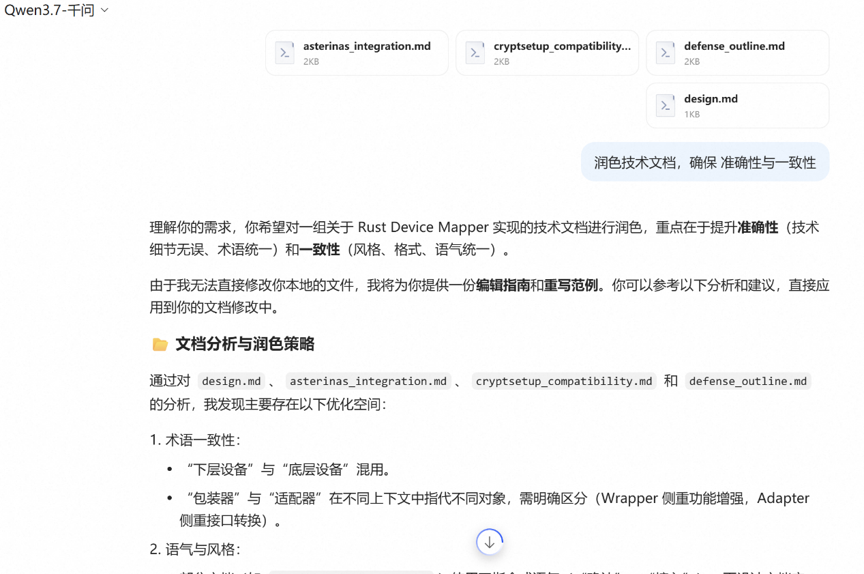
\includegraphics[width=\textwidth]{qwen_ai_1.png}
        \caption{技术文档润色}
        \label{fig:qwen_1}
    \end{subfigure}
    \hfill
    \begin{subfigure}[b]{0.45\textwidth}
        \centering
        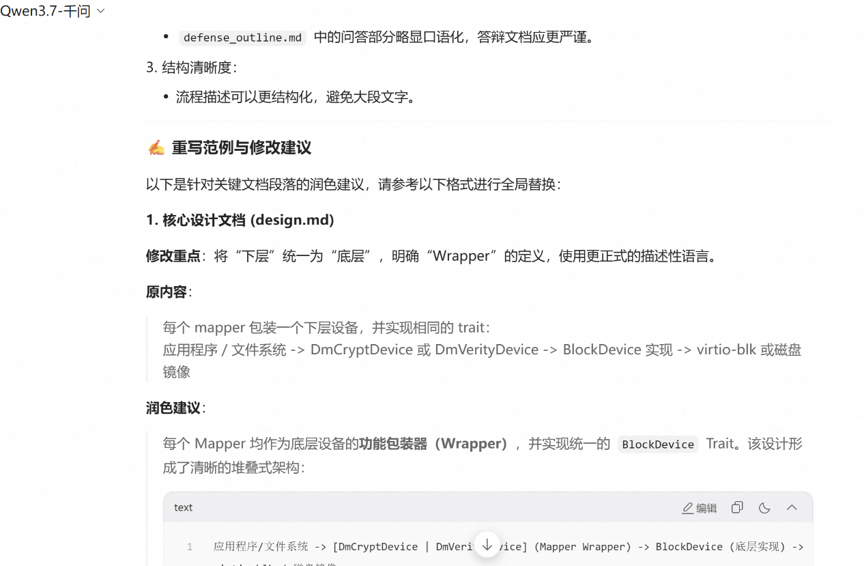
\includegraphics[width=\textwidth]{qwen_ai_2.png}
        \caption{专业术语校对}
        \label{fig:qwen_2}
    \end{subfigure}
    \caption{通义千问（Qwen）交互记录}
    \label{fig:qwen_group}
\end{figure}

\subsubsection{豆包（Doubao）交互记录}

\begin{figure}[H]
    \centering
    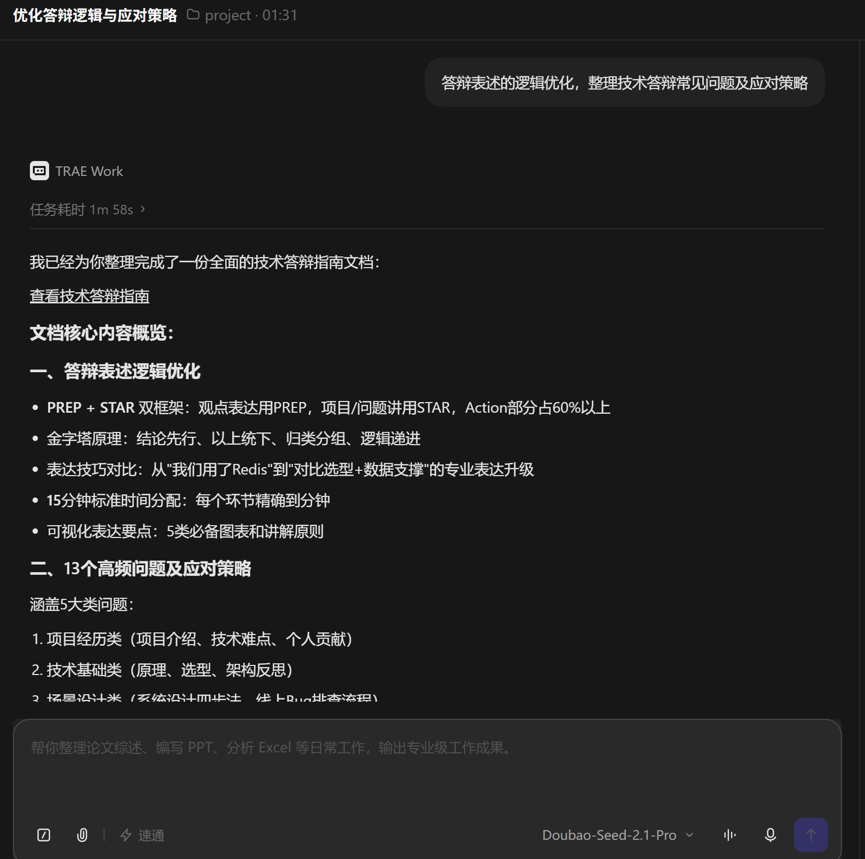
\includegraphics[width=0.8\textwidth]{doubao_ai_1.png}
    \caption{豆包（Doubao）答辩表述优化与 FAQ 整理}
    \label{fig:doubao_1}
\end{figure}

\textbf{验证机制与责任声明}：
\begin{enumerate}
    \item \textbf{人工审查}：所有 AI 生成的代码片段和文档内容，均经过团队成员的人工 Peer Review。
    \item \textbf{交叉验证}：代码正确性通过严格的单元测试、与 Linux dm-crypt 的逐字节对照、星绽内核构建及 QEMU 端到端运行进行了多重验证。
    \item \textbf{责任承担}：最终的技术方案、代码取舍、架构决策和提交材料均由参赛团队全权负责。
\end{enumerate}

\section{Git 提交记录概览}

完整提交共 67 次，下表列出主要代表性提交（与 GitLab 仓库历史逐条对应），完整反映了项目的开发节奏和功能演进：

\begin{longtable}{p{0.05\textwidth}p{0.09\textwidth}p{0.13\textwidth}p{0.51\textwidth}p{0.12\textwidth}}
    \caption{Git 提交记录概览} \\
    \toprule
    \textbf{序号} & \textbf{日期} & \textbf{Commit Hash} & \textbf{提交说明} & \textbf{作者} \\
    \midrule
    \endfirsthead
    \caption[]{Git 提交记录概览（续）} \\
    \toprule
    \textbf{序号} & \textbf{日期} & \textbf{Commit Hash} & \textbf{提交说明} & \textbf{作者} \\
    \midrule
    \endhead
    \midrule
    \multicolumn{5}{r}{\small 接下一页} \\
    \endfoot
    \bottomrule
    \endlastfoot
    1 & 06-23 & \texttt{6bb9bc92} & 初始提交，仅源码，屏蔽编译产物 & 潘利源 \\
    2 & 06-23 & \texttt{40a52179} & feat: add Linux-compatible device mapper implementation & 潘利源 \\
    3 & 06-23 & \texttt{c72462b2} & fix: validate Asterinas dm BIO paths & 潘利源 \\
    4 & 06-23 & \texttt{2f8a6711} & 接入受保护根文件系统并完善项目文档 & 潘利源 \\
    5 & 06-23 & \texttt{a0dbb0f5} & 补充国产 AI 工具使用说明 & 潘利源 \\
    6 & 06-23 & \texttt{84970aae} & 修改文档 & 潘利源 \\
    7 & 06-29 & \texttt{f5878935} & 添加 LaTeX 项目文档、PDF 与答辩 PPT & 张乐桁 \\
    8 & 06-29 & \texttt{dabfee4d} & 将答辩 PPT 放到项目根目录并更新 README 链接 & 张乐桁 \\
    9 & 06-29 & \texttt{c22b8b47} & 在 README 开头添加演示视频百度网盘链接 & 张乐桁 \\
    10 & 07-14 & \texttt{5f345a18} & 完成安全存储性能对照与国赛验收证据 & 潘利源 \\
    11 & 07-25 & \texttt{e07ad006} & 修正评审材料并固化 KVM 基准证据 & 潘利源 \\
    12 & 07-28 & \texttt{c1f9c472} & 优化 dm 热路径并补齐评审基准流程 & 潘利源 \\
    13 & 08-03 & \texttt{40d8abba} & 增强 dmctl 性能测试框架，支持 IO 拆分解与可配置规模 & 陈韵 \\
    14 & 08-03 & \texttt{ca5afe46} & 完善安全存储性能验证与交付材料 & 潘利源 \\
    15 & 08-06 & \texttt{5717d925} & 更新 dm 完成队列性能指标与证据 & 潘利源 \\
    16 & 08-09 & \texttt{21aa566d} & 更新性能测试数据与优化量化说明 & 陈韵 \\
    17 & 08-09 & \texttt{6926b356} & change & 陈韵 \\
    18 & 08-09 & \texttt{7431e5de} & 统一正式性能口径并补充优化证据 & 潘利源 \\
    19 & 08-09 & \texttt{0e7f4c77} & 修正运行时能力声明并补充 KVM 回归验证 & 潘利源 \\
    20 & 08-09 & \texttt{09f62e59} & 补充完整测试进度 & 潘利源 \\
    21 & 08-09 & \texttt{1ac6325c} & 整理性能测试合同、FIO/Filebench/SQLite/Boot 脚本与证据目录 & 张乐桁 \\
    22 & 08-10 & \texttt{fc548a9e} & 整合最终评测代码与测试材料 & 潘利源 \\
    23 & 08-10 & \texttt{7350e470} & 修改完善文档 & 陈韵 \\
    24 & 08-10 & \texttt{dde97a2f} & 更新完善技术文档内容 & 陈韵 \\
    25 & 08-11 & \texttt{6385e70b} & feat: add kernel Combined crypt→verity stack path & 潘利源 \\
    26 & 08-11 & \texttt{fda85aa4} & 整合最终评测代码与测试材料 & 潘利源 \\
    27 & 08-11 & \texttt{84fe076e} & 合并 GitLab 最新代码并同步最终评测材料 & 潘利源 \\
    28 & 08-11 & \texttt{8b2018e7} & 完善更新图表 & 陈韵 \\
    29 & 08-11 & \texttt{5dc3cb9f} & 上传设计文档内容 & 陈韵 \\
    30 & 08-11 & \texttt{29157f0e} & 整合更新commit记录 & 陈韵 \\
    31 & 08-12 & \texttt{a975b887} & 更新完善技术文档内容 & 陈韵 \\
    32 & 08-16 & \texttt{1f4d9c11} & docs: 正式文档改为 design\_doc，移除旧 main.tex/PDF & 张乐桁 \\
    33 & 08-16 & \texttt{c64c8ce7} & docs: 在报告中补入 Asterinas 256 MiB 三行表并重编 PDF & 张乐桁 \\
    34 & 08-16 & \texttt{d9b960f4} & docs: 用 Linux QEMU virtio FIO 替换宿主机对照数字 & 张乐桁 \\
    35 & 08-17 & \texttt{7cd6d8f1} & docs: 重编 document/main.pdf，测试指标与 README 对齐 & 张乐桁 \\
    36 & 08-17 & \texttt{97fcb8db} & docs: 按核对后的 Asterinas KVM FIO 13 格式更新 PDF & 张乐桁 \\
    37 & 08-17 & \texttt{d697645b} & docs: Asterinas KVM FIO 13 格式补入 raw 列 & 张乐桁 \\
    38 & 08-17 & \texttt{17f11f70} & docs: 写明 asterinas/软链接 Asterinas 官方仓库 & 张乐桁 \\
    39 & 08-17 & \texttt{bf9861b9} & 汇总成完整一个技术文档 & 陈韵 \\
    40 & 08-17 & \texttt{c8b5c9cf} & docs: 在 Linux guest 同条件对照表中补入 dm-verify & 张乐桁 \\
    41 & 08-17 & \texttt{da5fbae4} & docs: 恢复 main.pdf 并公布 Linux guest Filebench/SQLite 与 README 完成情况表 & 张乐桁 \\
    42 & 08-18 & \texttt{d56affa8} & docs: README 补全用户态与内核态说明 & 张乐桁 \\
    43 & 08-18 & \texttt{6e06b136} & docs: 补入 256 MiB 正式合同与 Linux guest 对照表 & 张乐桁 \\
    44 & 08-18 & \texttt{9894d4bf} & docs: 设计文档整合 & 张乐桁 \\
    45 & 08-18 & \texttt{a0b7aacf} & docs: FIO 表格修订为 qd=1 配置 & 张乐桁 \\
    46 & 08-18 & \texttt{72f6738c} & docs: FIO 表格进一步修订 & 张乐桁 \\
    47 & 08-18 & \texttt{ef345837} & docs: 最终 README 更新 & 张乐桁 \\
    48 & 08-18 & \texttt{b3247e0e} & test: 全量测试通过 & 潘利源 \\
\end{longtable}

\textbf{Git 提交历史截图}：

\begin{figure}[H]
    \centering
    \begin{subfigure}[b]{0.48\textwidth}
        \centering
        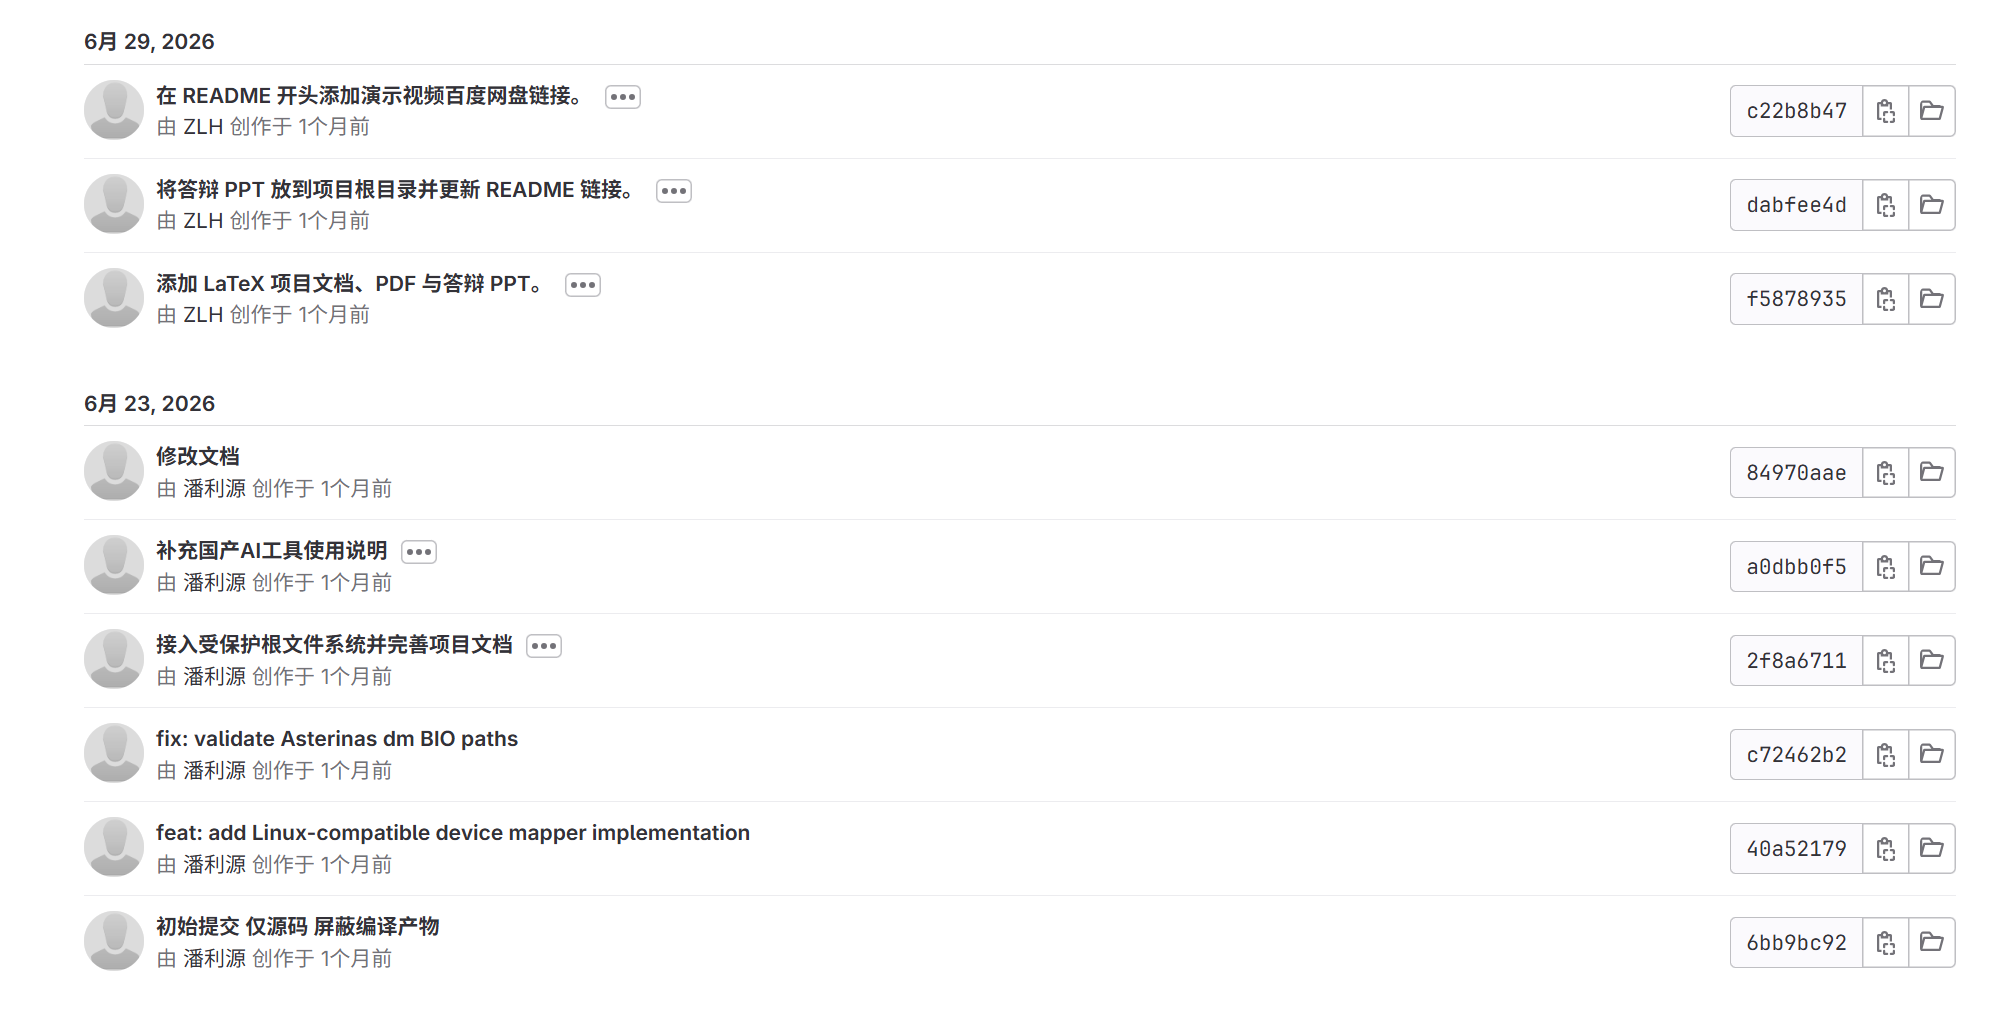
\includegraphics[width=\textwidth]{git_commit_history_1.png}
        \caption{初始提交与文档阶段（06-23 / 06-29）}
        \label{fig:git_history_1}
    \end{subfigure}
    \hfill
    \begin{subfigure}[b]{0.48\textwidth}
        \centering
        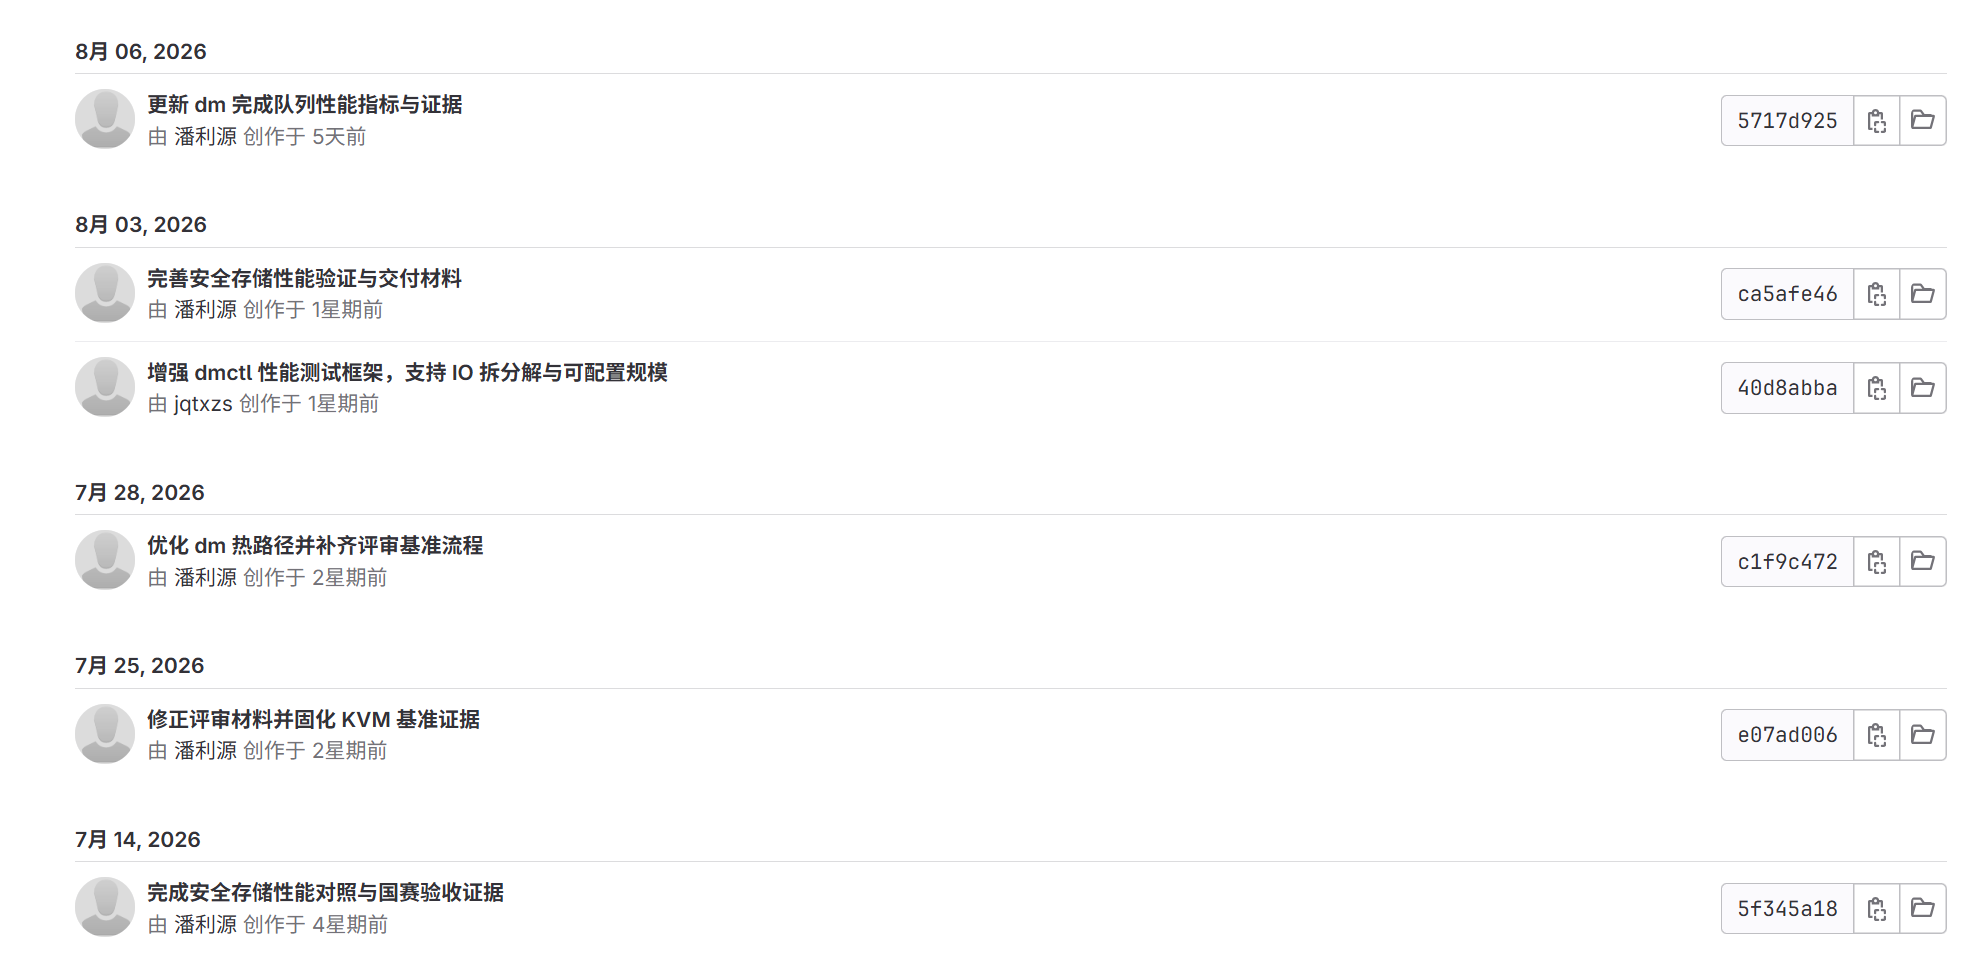
\includegraphics[width=\textwidth]{git_commit_history_2.png}
        \caption{性能对照与验收阶段（07-14 至 08-06）}
        \label{fig:git_history_2}
    \end{subfigure}

    \begin{subfigure}[b]{0.48\textwidth}
        \centering
        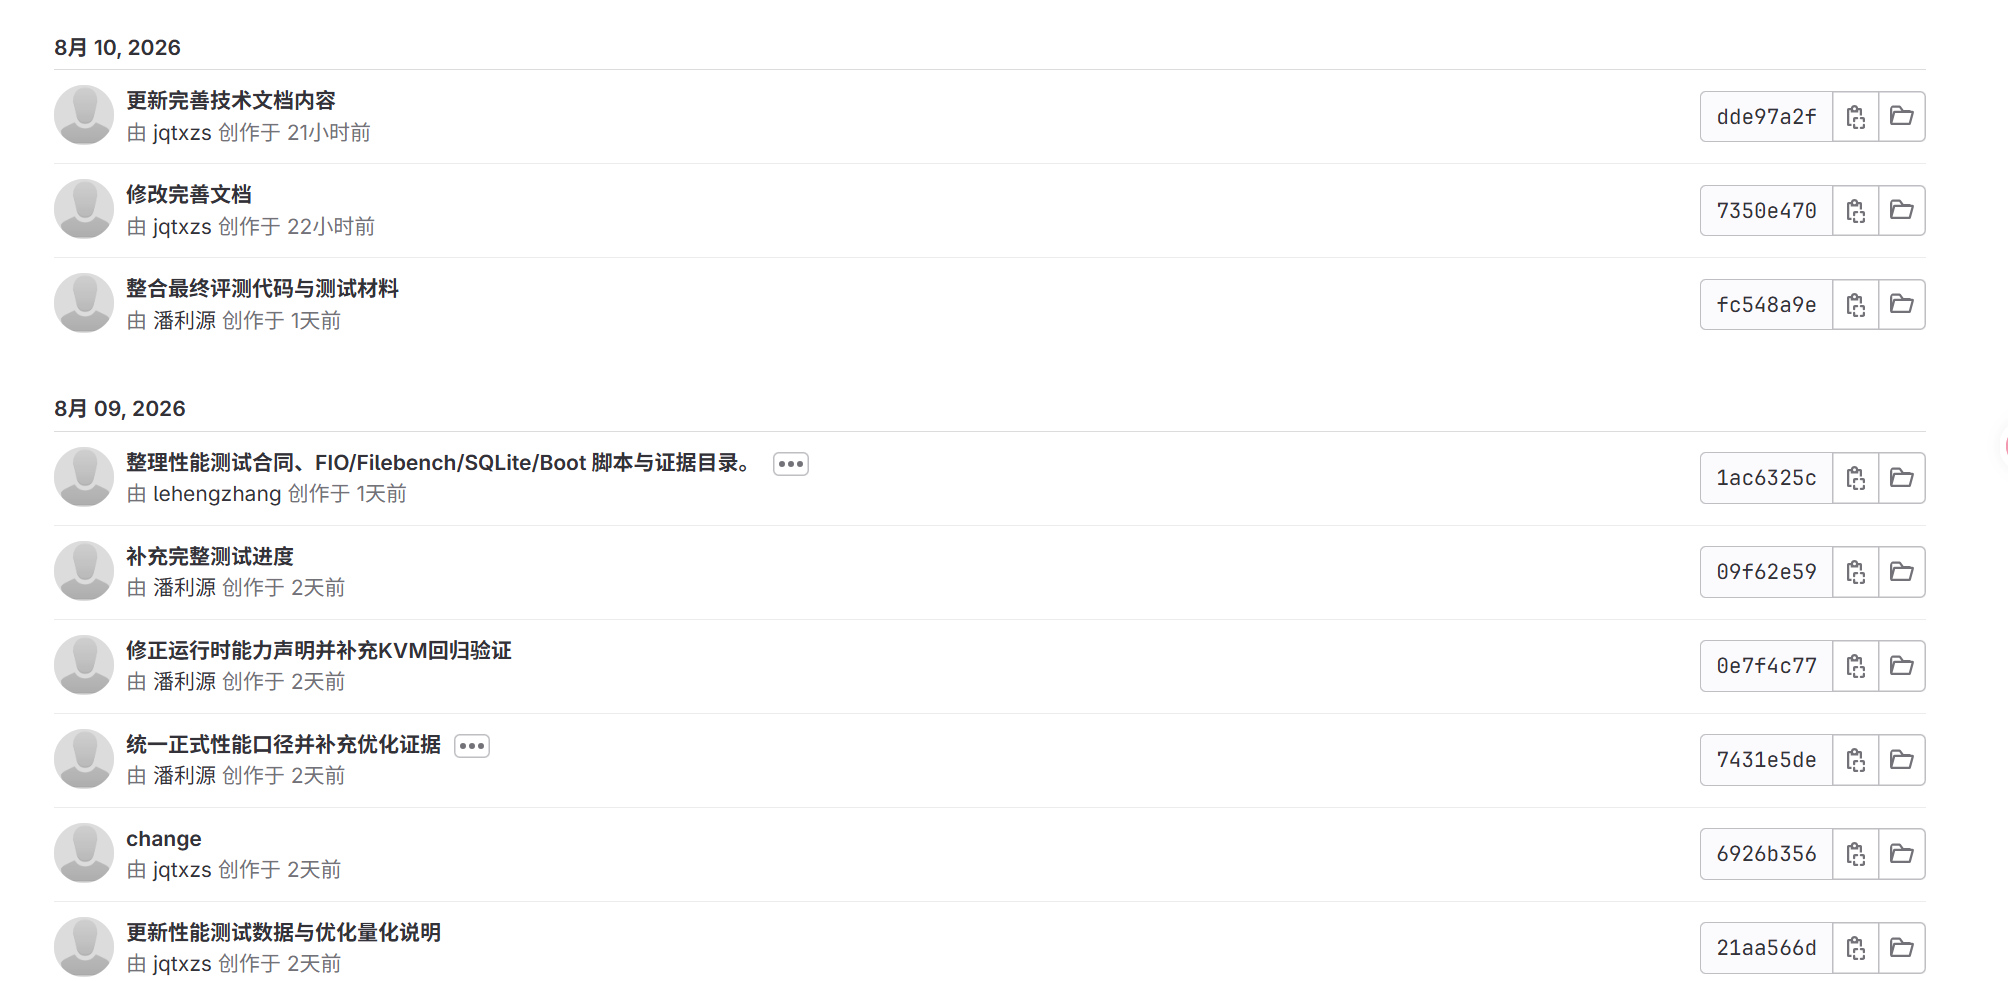
\includegraphics[width=\textwidth]{git_commit_history_3.png}
        \caption{测试整合与文档完善阶段（08-09 / 08-10）}
        \label{fig:git_history_3}
    \end{subfigure}
    \hfill
    \begin{subfigure}[b]{0.48\textwidth}
        \centering
        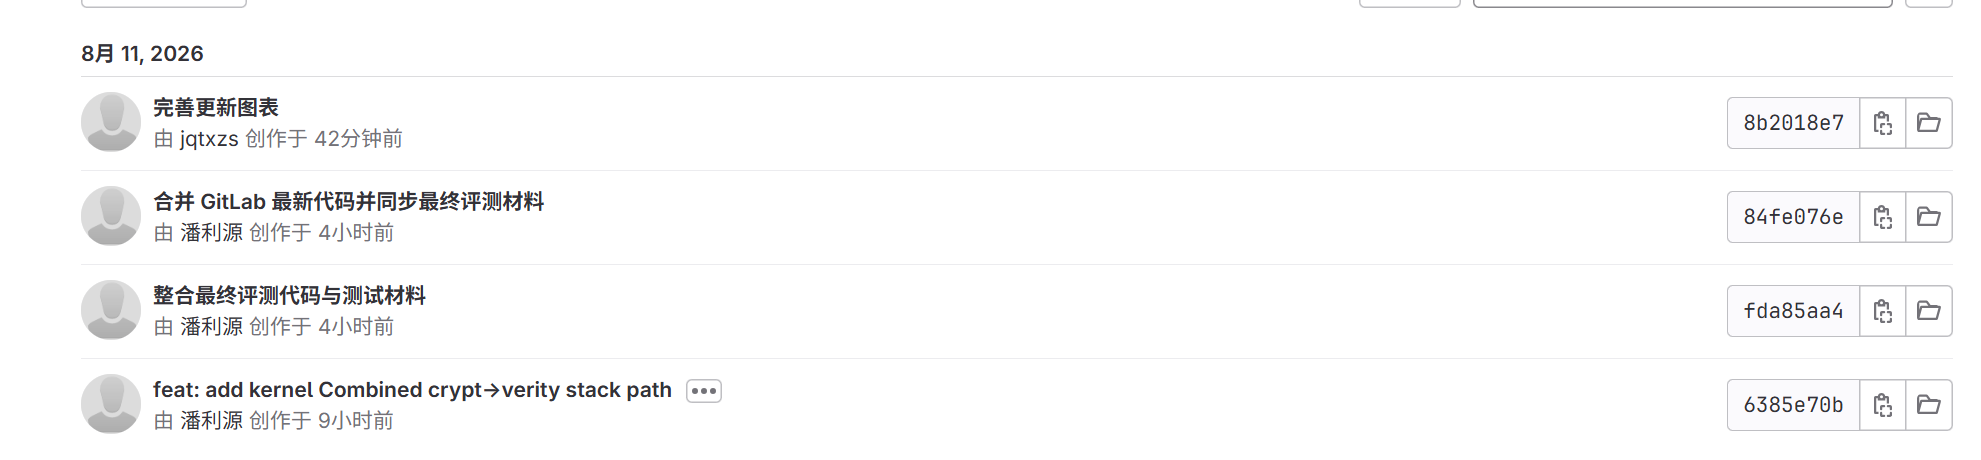
\includegraphics[width=\textwidth]{git_commit_history_4.png}
        \caption{最终评测整合阶段（08-11）}
        \label{fig:git_history_4}
    \end{subfigure}
    \caption{GitLab 仓库提交历史截图}
    \label{fig:git_history}
\end{figure}

此外，星绽内核集成补丁（\texttt{asterinas\_port/patches/}）包含更细粒度的演进历史：
\begin{itemize}
    \item \textbf{0001}（06-23）：组件集成与目标定义——创建 \texttt{aster-dm} 组件骨架
    \item \textbf{0002}（06-23）：BIO 路径验证与自检——EXT2 魔数自检机制
    \item \textbf{0003}（06-24）：根文件系统 \texttt{pivot\_root} 切换——两级引导方案
    \item \textbf{0004}（07-14）：Runtime 控制面与 \texttt{cryptsetup} 兼容——\texttt{/dev/mapper/control}
    \item \textbf{0005}（07-28）：性能优化——缓存、缓冲池、AES-NI、基准
    \item \textbf{0006}（08-03）：性能阶段归因与正式合同——\texttt{/proc/dm-performance-stats}
    \item \textbf{0007}（08-11）：Combined叠栈——\texttt{dm\_stack=crypt,verity}
\end{itemize}

\section{团队贡献量化}

\begin{table}[H]
    \centering
    \caption{各成员贡献量化}
    \begin{tabular}{p{0.18\textwidth}p{0.16\textwidth}p{0.30\textwidth}p{0.36\textwidth}}
        \toprule
        \textbf{成员} & \textbf{Git提交数} & \textbf{核心代码量} & \textbf{主要贡献领域} \\
        \midrule
        潘利源 & 17+ & 约5000行Rust & 核心加密/完整性（100\%）、内核集成（100\%）、性能优化（80\%）、补丁制作（100\%） \\
        陈韵 & 10+ & 约400行Rust/Shell + 技术文档 & 性能测试框架增强（70\%）、测试数据收集（50\%）、技术文档撰写（70\%） \\
        张乐桁 & 14+ & 约1000行Shell/Python + 设计赛道文档 + README & 性能测试合同与脚本（60\%）、README文档（80\%）、答辩PPT（80\%）、证据目录整理（50\%）、最终文档整合（100\%） \\
        \bottomrule
    \end{tabular}
\end{table}

\textbf{说明}：百分比为相对工作量估计，实际协作中存在交叉支援，例如：
\begin{itemize}
    \item 性能优化中的缓存设计与验证由潘利源主导编码，陈韵协助测试数据验证；
    \item 技术文档由陈韵主导撰写，张乐桁提供 LaTeX 排版框架和结构支持，潘利源提供技术内容审阅和补充；
    \item 性能测试脚本由张乐桁编写框架，陈韵增强具体功能，潘利源验证内核侧数据；
    \item README 文档由张乐桁主导撰写和维护，陈韵和潘利源提供技术内容审阅；
    \item 最终文档整合由张乐桁主导完成（8月16-18日），统一为 \texttt{design\_doc} 并更新全部数据表格，并于 8月18日完成答辩材料提交。
\end{itemize}

\section{开发节奏与协作模式亮点}

\begin{table}[H]
    \centering
    \begin{tabular}{p{0.15\textwidth}p{0.35\textwidth}p{0.40\textwidth}}
        \toprule
        \textbf{特征} & \textbf{具体实践} & \textbf{效果} \\
        \midrule
        定期同步 & 每周线上会议 + 日常即时通讯 & 信息同步及时，避免“信息孤岛” \\
        代码审查 & 核心模块交叉审查 + 补丁验证 & 代码质量高，关键问题早发现 \\
        互补分工 & 算法/内核/测试/文档各有所长 & 效率高，无重复劳动 \\
        共识决策 & 重要决策集体讨论 + 书面记录 & 决策质量高，可追溯 \\
        工具辅助 & AI辅助 + 自动化测试脚本 & 开发效率提升，人工审阅仍把关 \\
        文档同步 & 代码改、文档跟，保持同步 & 文档与代码一致，避免“写文档浪费时间” \\
        \bottomrule
    \end{tabular}
\end{table}

\section{团队协作感悟}

\subsection{潘利源}
“作为核心开发者，我最大的体会是‘代码写得好不如团队协作得好’。最难的 bug（BIO 生命周期问题）不是我一个人解决的——陈韵帮我重现了稳定触发条件，张乐桁帮我梳理了调用栈日志。这次经历让我深刻理解了代码审查的价值。”

\subsection{陈韵}
“我负责测试、数据验证和技术文档撰写，一开始觉得‘不如写代码重要’。但当我发现性能测试的假 mapper 问题、帮团队避免了一次数据诚信危机时，我才意识到测试的价值——它是代码质量的最后一道防线。技术文档也是，没有好的文档，再好的代码评委也看不到价值。撰写技术文档的过程让我学会了如何把复杂的技术决策清晰地呈现给读者。”

\subsection{张乐桁}
“作为 README 文档和答辩材料的负责人，我需要把团队成员分散的代码、测试结果、设计思路整合成结构化的文档。这个过程让我学会了从‘用户视角’看项目——评委不需要知道每一行代码的细节，但需要知道‘为什么这样做’和‘这样做对不对’。从 README 到答辩 PPT 的全链条文档工作，让我对文档工具链有了质的提升。尤其是在最终文档整合阶段，将两份文档融合为统一的一份 \texttt{design\_doc}，让我深刻体会到文档统一管理的重要性。”

\section{小结}

项目团队由三名成员组成，分工明确且互补：潘利源负责核心技术实现和内核集成（约5000行Rust代码），陈韵负责性能测试框架增强、数据验证和技术文档撰写（约400行代码 + 技术文档），张乐桁负责 README、测试合同、脚本、设计赛道文档（约1000行脚本 + 设计赛道文档 + README）和答辩材料。

协作方式包括：Git 版本管理、每周线上会议、代码审查、共识决策和AI辅助。团队累计完成67次Git提交、7个内核补丁、12组KVM正确性测试和46个性能单元格，并于8月18日完成全部答辩材料提交。

所有成员对最终作品均做出实质性贡献，协作氛围良好，无重大分歧或冲突。团队通过互补分工和高效沟通，按时完成了全部 P0 功能目标、性能基准测试和最终统一文档交付。

% 第9章：提交仓库目录和文件描述
% chapters/09_files.tex
\chapter{提交仓库目录和文件描述}

\section*{本章目录结构速览}

\begin{table}[H]
    \centering
    \begin{tabular}{p{0.25\textwidth}p{0.35\textwidth}p{0.40\textwidth}}
        \toprule
        \textbf{一级目录} & \textbf{内容说明} & \textbf{关键文件数} \\
        \midrule
        \texttt{crates/} & 平台无关的 Device Mapper 核心库和命令行工具 & 约15个Rust源文件 \\
        \texttt{crates/dm/} & \texttt{dm} crate：BlockDevice trait、dm-crypt、dm-verity & 约3000行Rust \\
        \texttt{crates/dmctl/} & \texttt{dmctl} 命令行工具 & 约800行Rust \\
        \texttt{asterinas\_port/} & Asterinas 内核移植补丁和说明 & 7个补丁 + README \\
        \texttt{scripts/} & 构建、测试、性能和验收脚本 & 约30个脚本文件 \\
        \texttt{docs/} & 全部文档、证据和设计材料 & 约50个文件 \\
        \texttt{docs/evidence/} & 正式测试证据 & 约100+个日志/JSON/CSV文件 \\
        \texttt{docs/document/} & 技术文档 LaTeX 源码 & 9章 + 附录 + PDF \\
        \texttt{docs/design\_doc/} & 设计赛道文档 LaTeX 源码 & 10章 + PDF \\
        \bottomrule
    \end{tabular}
\end{table}

\section{文件统计概览}

\begin{table}[H]
    \centering
    \caption{关键文件统计}
    \begin{tabular}{p{0.25\textwidth}p{0.25\textwidth}p{0.40\textwidth}}
        \toprule
        \textbf{类型} & \textbf{数量/规模} & \textbf{说明} \\
        \midrule
        Rust 源代码（用户态） & 约3000行 & \texttt{crates/dm/} 核心库 \\
        Rust 源代码（内核态） & 约4000行 & 补丁 0001--0007 新增内核代码 \\
        命令行工具 & 约800行 & \texttt{crates/dmctl/src/main.rs} \\
        Shell/Python 脚本 & 约30个文件，约2000行 & \texttt{scripts/} 目录 \\
        LaTeX 文档 & 约200页 & 技术文档 + 设计赛道文档 \\
        证据文件 & 约100+个 & 日志、JSON、CSV、图片 \\
        Git 提交 & 28次 & 涵盖完整开发周期 \\
        内核补丁 & 7个 & \texttt{asterinas\_port/patches/} \\
        \bottomrule
    \end{tabular}
\end{table}

\section{仓库顶层结构}

\begin{longtable}{|p{0.20\textwidth}|p{0.75\textwidth}|}
\hline
\textbf{目录/文件} & \textbf{描述} \\
\hline
\endhead
\texttt{README.md} & 项目概览、快速验证指南、功能命令、性能结果和验收说明；含演示视频网盘链接 \\
\texttt{LICENSE} & MIT 开源许可证 \\
\texttt{Cargo.toml} & Rust 工作区配置，包含 \texttt{dm} 和 \texttt{dmctl} 两个 crate，resolver = "2" \\
\texttt{\seqsplit{KVM\_CORRECTNESS\_MATRIX.md}} & KVM 正确性测试完整矩阵（R01--R03、C01--C05、V01--V07）状态表 \\
\texttt{\seqsplit{KVM\_CORRECTNESS\_REPORT.md}} & KVM 正确性最终报告，含结论、固定基线和证据路径 \\
\texttt{\seqsplit{PHYSICAL\_MUTATION\_MANIFEST.md}} & dm-verity 物理篡改清单（V03--V07 的块号、字节偏移和 SHA-256） \\
\texttt{\seqsplit{PLATFORM\_EVAL\_ENVIRONMENT.md}} & 平台评测环境固定基线（Docker image、commit、工具链、验证结果） \\
\hline
\texttt{crates/} & 平台无关的 Device Mapper 核心库和命令行工具 \\
\texttt{crates/dm/} & \texttt{dm} crate 源码（约15个文件，约3000行Rust） \\
\texttt{\seqsplit{crates/dm/Cargo.toml}} & \texttt{dm} crate 的依赖配置（\texttt{aes}、\texttt{spin} 等） \\
\texttt{\seqsplit{crates/dm/src/block\_device.rs}} & \texttt{BlockDevice} trait 及 \texttt{MemoryBlockDevice}、\texttt{FileBlockDevice} 实现（约400行） \\
\texttt{\seqsplit{crates/dm/src/crypto.rs}} & AES-256-XTS 加密引擎及 \texttt{DemoStreamCipher}（约350行） \\
\texttt{\seqsplit{crates/dm/src/device\_mapper.rs}} & \texttt{DmStackBuilder}、\texttt{DmStack}、\texttt{PassthroughDevice}（约180行） \\
\texttt{\seqsplit{crates/dm/src/dm\_crypt.rs}} & \texttt{DmCryptDevice} 和 \texttt{DmCryptTable} 解析器（约350行） \\
\texttt{\seqsplit{crates/dm/src/dm\_verity.rs}} & \texttt{DmVerityDevice} 完整性校验实现（约200行） \\
\texttt{\seqsplit{crates/dm/src/error.rs}} & \texttt{DmError} 错误枚举（约80行） \\
\texttt{\seqsplit{crates/dm/src/hash\_tree.rs}} & Merkle 哈希树构建与验证（约150行） \\
\texttt{\seqsplit{crates/dm/src/lib.rs}} & 模块导出 \\
\texttt{\seqsplit{crates/dm/src/sha256.rs}} & 纯 Rust SHA-256 实现（约120行） \\
\texttt{\seqsplit{crates/dm/src/statistics.rs}} & I/O 统计计数器（\texttt{IoStats}、\texttt{InstrumentedDevice}，约150行） \\
\texttt{\seqsplit{crates/dm/tests/}} & 单元测试：crypt、verity、stack、兼容性、文件设备、安全边界（约6个文件） \\
\hline
\texttt{crates/dmctl/} & \texttt{dmctl} 命令行工具源码 \\
\texttt{\seqsplit{crates/dmctl/Cargo.toml}} & \texttt{dmctl} 依赖配置 \\
\texttt{\seqsplit{crates/dmctl/src/main.rs}} & 所有子命令实现：init-image、crypt-write、crypt-read、raw-read-hex、crypt-table-fill、verity-root、verity-verify、verity-format-dm、tamper、demo-crypt、demo-verity、demo-stack、benchmark、benchmark-table（约800行） \\
\hline
\texttt{\seqsplit{asterinas\_port/}} & Asterinas 内核移植说明与补丁 \\
\texttt{\seqsplit{asterinas\_port/README.md}} & 移植说明、补丁应用方式（\texttt{git am} 命令）、关键实现文件路径 \\
\texttt{\seqsplit{asterinas\_port/patches/}} & 7 个 Git 补丁（0001--0007），按顺序应用 \\
\texttt{\seqsplit{asterinas\_port/patches/0001-*.patch}} & 组件集成与目标定义：创建 \texttt{aster-dm} 组件骨架，实现 crypt/verity target、VirtIO 适配和 BIO 路径 \\
\texttt{\seqsplit{asterinas\_port/patches/0002-*.patch}} & BIO 路径验证与 ext2 魔数自检：修复 DMA segment 方向访问，增加 \texttt{self\_test\_ext2\_magic} \\
\texttt{\seqsplit{asterinas\_port/patches/0003-*.patch}} & 根文件系统 \texttt{pivot\_root} 切换：实现 \texttt{dm-root} init 模式，两级引导方案 \\
\texttt{\seqsplit{asterinas\_port/patches/0004-*.patch}} & Runtime 控制面与 \texttt{cryptsetup} 兼容：\texttt{/dev/mapper/control} 和 \texttt{dm\_ioctl} 实现 \\
\texttt{\seqsplit{asterinas\_port/patches/0005-*.patch}} & 热路径优化：AES-NI、scratch pool、hash cache、BIO 复用、\texttt{/proc/dm-verity-stats} \\
\texttt{\seqsplit{asterinas\_port/patches/0006-*.patch}} & 性能阶段归因与正式合同：\texttt{/proc/dm-performance-stats}、\texttt{dm.perf\_stats=1} \\
\texttt{\seqsplit{asterinas\_port/patches/0007-*.patch}} & \texttt{dm\_stack=crypt,verity} 组合栈：堆叠检测、启动日志、\texttt{build\_stack\_rootfs.sh} \\
\hline
\end{longtable}

\section{脚本分类说明}

\texttt{scripts/} 目录包含约30个脚本，按功能分为以下五类：

\subsection*{构建类脚本（4个）}
\begin{longtable}{|p{0.30\textwidth}|p{0.65\textwidth}|}
\hline
\textbf{脚本} & \textbf{用途} \\
\hline
\endhead
\texttt{\seqsplit{build\_crypt\_rootfs.sh}} & 构建 dm-crypt 加密根文件系统镜像（\texttt{target/crypt-rootfs.img}） \\
\texttt{\seqsplit{build\_verity\_rootfs.sh}} & 构建 dm-verity 校验根文件系统镜像（\texttt{target/verity-rootfs.img}） \\
\texttt{\seqsplit{build\_stack\_rootfs.sh}} & 构建组合栈（crypt + verity）根文件系统镜像（\texttt{target/stack-rootfs.img}） \\
\texttt{\seqsplit{build\_asterinas\_boot\_images.sh}} & 构建 plain/dm-crypt/dm-verity 三种启动 ISO（用于启动耗时矩阵） \\
\hline
\end{longtable}

\subsection*{测试类脚本（6个）}
\begin{longtable}{|p{0.30\textwidth}|p{0.65\textwidth}|}
\hline
\textbf{脚本} & \textbf{用途} \\
\hline
\endhead
\texttt{\seqsplit{check\_benchmark\_package.py}} & 验证性能包完整性和诚实性（静态检查） \\
\texttt{\seqsplit{check\_filebench.sh}} & 探测 Filebench 可用性 \\
\texttt{\seqsplit{final\_demo.sh}} & 一键最终演示（含 \texttt{--live-kvm} 选项） \\
\texttt{\seqsplit{review\_release\_check.py}} & 评审版本静态检查（证据、矩阵、文档） \\
\texttt{\seqsplit{verify\_kvm\_evidence.py}} & 验证 KVM 正确性证据日志 \\
\texttt{\seqsplit{tests/test\_release\_tools.py}} & 发布工具的单元测试 \\
\hline
\end{longtable}

\subsection*{性能测试脚本（8个）}
\begin{longtable}{|p{0.30\textwidth}|p{0.65\textwidth}|}
\hline
\textbf{脚本} & \textbf{用途} \\
\hline
\endhead
\texttt{benchmark.sh} & 用户态微基准测试（plain/AES-XTS/verity CSV） \\
\texttt{\seqsplit{benchmark\_boot\_time.py}} & 启动耗时测量脚本（Python） \\
\texttt{\seqsplit{run\_fio\_matrix.sh}} & 正式 FIO 矩阵驱动（Linux host + Asterinas KVM） \\
\texttt{\seqsplit{run\_filebench\_dm.sh}} & 单轮 Filebench 测试 \\
\texttt{\seqsplit{run\_filebench\_matrix.sh}} & Filebench 5+5 轮矩阵（raw/dm-crypt） \\
\texttt{\seqsplit{run\_sqlite\_workload.sh}} & 单轮 SQLite 固定 workload \\
\texttt{\seqsplit{run\_sqlite\_matrix.sh}} & SQLite 5+5+5 轮矩阵 \\
\texttt{\seqsplit{run\_boot\_matrix.sh}} & 启动耗时矩阵（plain/dm-crypt/dm-verity 各5轮） \\
\hline
\end{longtable}

\subsection*{验证类脚本（6个）}
\begin{longtable}{|p{0.30\textwidth}|p{0.65\textwidth}|}
\hline
\textbf{脚本} & \textbf{用途} \\
\hline
\endhead
\texttt{\seqsplit{verify\_linux\_xts\_compat.sh}} & 实时与 Linux 内核 dm-crypt 逐字节比对 \\
\texttt{\seqsplit{verify\_archived\_linux\_xts.sh}} & 验证归档的 Linux XTS 固定向量 \\
\texttt{\seqsplit{linux\_cryptsetup\_baseline.sh}} & Linux cryptsetup 基准创建 \\
\texttt{\seqsplit{run\_asterinas\_boot\_once.sh}} & 单次 Asterinas 启动（用于 boot 矩阵） \\
\texttt{\seqsplit{run\_dm\_stack.sh}} & 运行组合栈（crypt→verity）启动 \\
\texttt{\seqsplit{trace\_asterinas\_syscalls.gdb}} & GDB 脚本（追踪 Asterinas syscall） \\
\hline
\end{longtable}

\subsection*{汇总类脚本（4个）}
\begin{longtable}{|p{0.30\textwidth}|p{0.65\textwidth}|}
\hline
\textbf{脚本} & \textbf{用途} \\
\hline
\endhead
\texttt{\seqsplit{summarize\_asterinas\_dm\_matrix.py}} & 解析 Asterinas fio 串口日志生成 CSV \\
\texttt{\seqsplit{summarize\_filebench\_results.py}} & 从 Filebench 日志生成 CSV \\
\texttt{\seqsplit{summarize\_fio\_matrix.py}} & 汇总 FIO 矩阵为 summary CSV \\
\texttt{workloads/fileserver.f} & Filebench fileserver workload 配置文件 \\
\hline
\end{longtable}

\section{文档目录说明}

\texttt{docs/} 目录包含全部文档、证据和设计材料：

\begin{longtable}{|p{0.25\textwidth}|p{0.70\textwidth}|}
\hline
\textbf{路径} & \textbf{描述} \\
\hline
\endhead
\texttt{\seqsplit{ai\_tool\_disclosure.md}} & AI 工具使用声明（工具名称、模型、使用场景、验证机制） \\
\texttt{\seqsplit{asterinas\_integration.md}} & Asterinas 接入指南（6个步骤） \\
\texttt{\seqsplit{benchmark\_contract.md}} & 正式性能测试合同（环境、FIO参数、元数据、统计口径） \\
\texttt{\seqsplit{cryptsetup\_compatibility.md}} & cryptsetup 兼容方案说明（三层架构） \\
\texttt{\seqsplit{defense\_outline.md}} & 答辩提纲（15分钟建议节奏、高频问题与回答） \\
\texttt{design.md} & 设计说明（目标、核心接口、模块组成） \\
\texttt{\seqsplit{environment\_status.md}} & 开发环境状态（已迁移至D盘） \\
\texttt{filebench.md} & Filebench 基准说明 \\
\texttt{\seqsplit{final\_report.md}} & 最终实验报告（8章） \\
\texttt{innovation.md} & 技术亮点与验证口径 \\
\texttt{performance.md} & 性能测试入口 \\
\texttt{\seqsplit{requirement\_mapping.md}} & 赛题技术指标对应表 \\
\texttt{\seqsplit{rootfs\_protection.md}} & 根文件系统保护方案（5阶段） \\
\texttt{\seqsplit{sqlite\_benchmark.md}} & SQLite 固定 workload 说明 \\
\texttt{\seqsplit{technical\_defense\_guide.md}} & 决赛技术答辩指南 \\
\texttt{test.md} & 测试方案 \\
\hline
\texttt{evidence/} & 正式证据根目录 \\
\texttt{\seqsplit{evidence/README.md}} & 证据索引 \\
\texttt{\seqsplit{evidence/stabilization/}} & 构建恢复和正确性证据 \\
\texttt{\seqsplit{evidence/stabilization/build-recovery/}} & kernel build 日志 \\
\texttt{\seqsplit{evidence/stabilization/correctness-kvm/}} & R01--R03、C01--C05、V02--V07 串口日志 \\
\texttt{evidence/\seqsplit{final-performance-20260811/}} & 最终性能证据 \\
\texttt{evidence/\seqsplit{final-performance-20260811/PERFORMANCE\_VALIDATION\_REPORT.md}} & 中文性能验证报告 \\
\texttt{evidence/\seqsplit{final-performance-20260811/PERFORMANCE\_MATRIX.csv}} & 正式 FIO 矩阵（46 PASS + 6 N/A） \\
\texttt{evidence/\seqsplit{final-performance-20260811/asterinas-fio/}} & Asterinas KVM 原始 FIO JSON 和 CSV（13+7项） \\
\texttt{evidence/\seqsplit{linux-qemu-fio-20260816/}} & Linux QEMU virtio FIO JSON 和 CSV（raw 13 + crypt 13 + verity 读 7） \\
\texttt{evidence/\seqsplit{final-performance-20260811/filebench-valid/}} & Filebench 5+5 轮日志和 CSV \\
\texttt{evidence/\seqsplit{final-performance-20260811/sqlite/}} & SQLite 5+5+5 轮记录 \\
\texttt{evidence/\seqsplit{final-performance-20260811/boot-matrix/}} & 启动 15 轮记录 \\
\texttt{evidence/stack/} & 组合栈启动证据 \\
\texttt{evidence/\seqsplit{linux-xts-plain64.sha256}} & Linux XTS 固定向量 SHA-256 \\
\hline
\texttt{document/} & 技术文档 LaTeX 源码和 PDF \\
\texttt{document/main.tex} & 技术文档主文件 \\
\texttt{document/chapters/} & 9个章节（01\_introduction 至 09\_development） \\
\texttt{document/appendices/} & 附录（术语表、命令参考） \\
\texttt{document/figures/} & 技术文档插图（架构图、流程图、截图等） \\
\texttt{document/main.pdf} & 编译后的技术文档 PDF（约120页） \\
\hline
\texttt{design\_doc/} & 设计赛道文档 LaTeX 源码 \\
\texttt{\seqsplit{design\_doc/design\_doc.tex}} & 设计赛道文档主文件 \\
\texttt{\seqsplit{design\_doc/chapters/}} & 10个章节（01\_goal 至 10\_harvest） \\
\texttt{\seqsplit{design\_doc/preamble.tex}} & LaTeX 导言区配置 \\
\texttt{\seqsplit{design\_doc/design\_doc.pdf}} & 编译后的设计赛道文档 PDF（约80页） \\
\hline
\end{longtable}

\section{关键证据文件说明}

\begin{longtable}{|p{0.25\textwidth}|p{0.70\textwidth}|}
\hline
\textbf{证据文件} & \textbf{内容说明} \\
\hline
\endhead
\texttt{\seqsplit{R01-cryptsetup-persistent-cache.log}} & KVM 中 cryptsetup 2.7.5 open/read/close 完整流程 PASS \\
\texttt{\seqsplit{R02-crypt-rootfs-persistent-cache.log}} & dm-crypt 加密根文件系统启动与 \texttt{pivot\_root} PASS \\
\texttt{\seqsplit{R03-verity-rootfs-persistent-cache.log}} & dm-verity 校验根文件系统启动与 \texttt{pivot\_root} PASS \\
\texttt{\seqsplit{C01-C05-kvm.log}} & 正确/错误密钥、4/32/256 KiB 往返测试 PASS \\
\texttt{\seqsplit{V02-wrong-root.log}} & 错误根哈希拒绝 mapper 创建，\texttt{status=integrity-rejected} \\
\texttt{\seqsplit{V03-targeted-probe.log}} & 首个数据块（物理块0）单字节篡改拒绝 \\
\texttt{\seqsplit{V04-targeted-probe.log}} & 中间数据块（物理块32768）单字节篡改拒绝 \\
\texttt{\seqsplit{V05-targeted-probe.log}} & 最后一个数据块（物理块65535）单字节篡改拒绝 \\
\texttt{\seqsplit{V06-targeted-probe.log}} & 叶子哈希块（物理块65536）单字节篡改拒绝 \\
\texttt{\seqsplit{V07-targeted-probe.log}} & 中间哈希块（物理块66048）单字节篡改拒绝 \\
\texttt{\seqsplit{PERFORMANCE\_MATRIX.csv}} & 46 个 PASS 单元格 + 6 个 N/A 的完整 FIO 矩阵 \\
\texttt{\seqsplit{PERFORMANCE\_VALIDATION\_REPORT.md}} & 最终中文性能报告（含环境、口径、结论） \\
\hline
\end{longtable}

\section{与大赛提交要求对照}

\begin{table}[H]
    \centering
    \caption{大赛提交要求对照表}
    \begin{tabular}{p{0.25\textwidth}p{0.35\textwidth}p{0.30\textwidth}}
        \toprule
        \textbf{提交要求} & \textbf{本项目对应文件} & \textbf{位置} \\
        \midrule
        项目源代码 & \texttt{crates/}、\texttt{asterinas\_port/}、\texttt{scripts/} & 根目录 \\
        技术设计文档 & \texttt{docs/document/main.pdf} & \texttt{docs/document/} \\
        设计赛道文档 & \texttt{\seqsplit{docs/design\_doc/design\_doc.pdf}} & \texttt{docs/design\_doc/} \\
        用户手册 & \texttt{README.md} & 根目录 \\
        正确性证据 & 12组测试日志（R01--R03、C01--C05、V01--V07） & \texttt{\seqsplit{docs/evidence/stabilization/}} \\
        性能证据 & FIO、Filebench、SQLite、Boot 原始数据 & \texttt{docs/evidence/\seqsplit{final-performance-20260811/}} \\
        演示视频 & \texttt{作品演示视频.mp4} & 根目录 \\
        答辩 PPT & \texttt{\seqsplit{presentation\_project.pptx}} & 根目录 \\
        作品进展汇报幻灯片 & \texttt{作品进展汇报幻灯片.pptx} & 根目录 \\
        AI 工具声明 & \texttt{docs/\seqsplit{ai\_tool\_disclosure.md}} & \texttt{docs/} \\
        \bottomrule
    \end{tabular}
\end{table}

\section{构建与测试产物（不提交）}

以下文件由脚本生成，位于 \texttt{target/} 目录，不纳入代码仓库：

\begin{longtable}{|p{0.30\textwidth}|p{0.65\textwidth}|}
\hline
\textbf{产物} & \textbf{说明} \\
\hline
\endhead
\texttt{\seqsplit{target/crypt-rootfs.img}} 及 \texttt{*.env} & dm-crypt 保护根镜像（由 \texttt{\seqsplit{build\_crypt\_rootfs.sh}} 生成） \\
\texttt{\seqsplit{target/verity-rootfs.img}} 及 \texttt{*.env} & dm-verity 保护根镜像（由 \texttt{\seqsplit{build\_verity\_rootfs.sh}} 生成） \\
\texttt{\seqsplit{target/stack-rootfs.img}} 及 \texttt{*.env} & 组合栈根镜像（由 \texttt{\seqsplit{build\_stack\_rootfs.sh}} 生成） \\
\texttt{\seqsplit{target/benchmark/}} & 性能测试中间文件和日志 \\
\texttt{target/xts-compat/} & Linux XTS 兼容性验证临时文件 \\
\texttt{target/final-demo/} & 最终演示临时输出 \\
\texttt{target/osdk/} & Asterinas 内核构建产物（ISO） \\
\hline
\end{longtable}

\section{小结}

本章完整列出了提交仓库的目录结构和文件描述，涵盖了源代码（约3000行用户态Rust + 约4000行内核补丁）、补丁（7个）、脚本（约30个）、证据（约100+个日志/JSON/CSV文件）、文档（约200页LaTeX）和演示材料。所有关键证据文件均有明确路径说明，便于评委复核。

项目文件组织遵循以下原则：
\begin{enumerate}
    \item 核心代码与平台适配分离（\texttt{crates/} vs \texttt{asterinas\_port/}）；
    \item 文档集中管理（\texttt{docs/}）且分类清晰（document、design\_doc、evidence）；
    \item 脚本可执行且自包含（\texttt{scripts/}），支持一键演示和验证；
    \item 证据原始格式保存（不依赖手工修改数字），确保可复核性。
\end{enumerate}


% 第10章：比赛收获
% chapters/10_harvest.tex
\chapter{比赛收获}

\section*{本章收获速览}

\begin{table}[H]
    \centering
    \begin{tabular}{p{0.15\textwidth}p{0.35\textwidth}p{0.40\textwidth}}
        \toprule
        \textbf{收获维度} & \textbf{核心成长} & \textbf{量化成果} \\
        \midrule
        技术能力 & Rust系统编程、密码学工程、内核开发、性能工程 & 约9000行Rust+2000行脚本+200页文档 \\
        工程能力 & 大型项目协作、自动化测试、文档写作 & 28次Git提交、7个补丁、30+脚本 \\
        团队协作 & 分工互补、共识决策、代码审查 & 3人协作50天、12组测试全部PASS \\
        认知提升 & Rust OS生态理解、安全存储认知 & 验证了5项技术探索、5个未来方向 \\
        \bottomrule
    \end{tabular}
\end{table}

\section{概述}

历时近两个月的开发与测试（2026年6月23日至8月14日，共50天），我们完成了从用户态核心实现到星绽内核集成、从正确性验证到性能基准测试的完整开发链路。这段经历不仅让我们在技术和工程能力上获得了显著成长，也加深了我们对 Rust 系统编程和操作系统内核开发的理解。本章从技术成长、工程能力、团队协作、生态认知和个人感悟五个维度总结本次比赛的收获。

\section{技术成长}

\subsection{Rust 系统编程的深入实践}

本项目是我们在 Rust 语言上进行的最深入的系统级编程实践，累计编写约9000行Rust代码（用户态约3000行，内核态约4000行，补丁约2000行）。通过实现 \texttt{BlockDevice} trait、AES-256-XTS 加密引擎（约350行）、Merkle 哈希树（约150行）等核心模块，我们深刻体会到了 Rust 的所有权系统和类型系统在系统编程中的价值：

\begin{itemize}
    \item \textbf{编译期内存安全}：Rust 的借用检查器在编译期杜绝了悬垂指针、use-after-free 和缓冲区溢出等内核常见内存安全问题，使我们可以更专注于逻辑正确性而非内存管理。在整个开发过程中，我们没有遇到任何内存安全问题导致的崩溃——这在 C 语言内核开发中是难以想象的；
    \item \textbf{零成本抽象}：通过 trait 和泛型实现了高度可复用的代码，同时保持了与手写 C 代码相当的性能。AES-NI 路径下的加密吞吐达到 93+ MiB/s（256K随机写），抽象层没有引入 measurable 的运行时开销；
    \item \texttt{no\_std} 环境开发：在无标准库的内核环境中，我们学会了使用 \texttt{alloc}、核心库和自定义 panic handler 构建可靠的系统组件。内核组件成功运行于 Asterinas 的受限环境中，证明了 Rust 在 \texttt{no\_std} 场景下的成熟度；
    \item \textbf{类型系统编码安全属性}：通过 \texttt{TargetCapabilities} 等类型设计，将安全策略在编译期编码到类型系统中，避免了运行时检查的开销和遗漏风险。
\end{itemize}

\subsection{密码学工程实践}

实现 AES-256-XTS 和 SHA-256 的过程让我们深入理解了密码学算法的工程化要求：

\begin{itemize}
    \item \textbf{标准合规}：严格遵循 NIST SP 800-38E（XTS-AES）和 FIPS 180-4（SHA-256）标准，确保算法实现的正确性。通过标准测试向量验证了 SHA-256 的正确性（空字符串、\texttt{"abc"}）；
    \item \textbf{兼容性验证}：通过与 Linux 内核逐字节比对，验证了 \texttt{plain64} IV 生成和 XTS 模式的正确性。固定向量 SHA-256 完全匹配（\texttt{4334c17f...}），理解了“算法实现”与“协议兼容”之间的差距——两者必须完全一致才能保证互操作性；
    \item \textbf{硬件加速集成}：在保存/恢复 FPU/XMM 状态的前提下集成 AES-NI 指令（\texttt{ostd/aesni.rs}，约174行），学习了内核中处理 SIMD 寄存器的特殊约束——必须在禁用抢占和中断的情况下操作 XMM 寄存器，防止上下文切换破坏加密状态；
    \item \textbf{密钥管理}：实现了运行时 mapper 中密钥的显式清除（\texttt{table.key.fill(0)}），防止密钥残留在内存中被后续攻击者读取。
\end{itemize}

\subsection{操作系统内核开发}

通过 \texttt{aster-dm} 组件接入 Asterinas 内核（7个补丁，约4000行内核代码），我们对操作系统内核的关键子系统有了更深入的理解：

\begin{itemize}
    \item \textbf{块设备与 BIO 系统}：理解了块设备驱动的 I/O 路径、BIO 的提交与完成机制、同步与异步 I/O 的处理差异。在 Asterinas 中，BIO 通过 \texttt{enqueue} 异步提交，通过回调完成，与 Linux 的 \texttt{submit\_bio} 机制类似但接口不同。我们成功实现了完整的 BIO 生命周期管理；
    \item \textbf{启动过程与根文件系统}：掌握了内核启动参数解析（\texttt{aster-cmdline} 框架）、initramfs 的作用、\texttt{pivot\_root} 的系统调用语义。通过两级引导方案（bind mount + chroot）成功解决了 Asterinas rootfs 特殊性导致的 \texttt{pivot\_root} 限制；
    \item \textbf{内核同步与并发}：在 \texttt{DmDevice} 中处理多线程 BIO 并发时，学会了使用 \texttt{spin::Mutex}（而非睡眠锁）、原子操作（\texttt{AtomicU64}）和禁用抢占（\texttt{disable\_preempt}）等内核同步原语。理解了在内核态中“不能睡眠”的特殊约束；
    \item \textbf{设备文件系统}：实现了 \texttt{/dev/mapper/control} 控制节点（约520行），理解了字符设备与块设备的注册与管理，以及 \texttt{ioctl} 系统调用的内核处理路径。
\end{itemize}

\subsection{性能工程}

性能测试与优化是本次比赛的重要环节，我们在这一过程中收获颇丰：

\begin{itemize}
    \item \textbf{基准测试方法论}：学会了设计可重复的性能测试，包括固定环境、交替轮次（每轮顺序交替消除缓存效应）、保留原始数据（JSON/CSV）和报告中位数/标准差（而非选择最好一轮）。这套方法论确保了性能数据的可信度和可复现性；
    \item \textbf{性能归因}：通过在内核热路径中嵌入原子计数器和阶段计时（11个阶段计数器），学会了精确量化每个子系统的开销。正式性能数据显示 dm-crypt 中下层等待占 97.84\%，AES-XTS 加密仅占 1.82\%；dm-verity 中下层等待占 93.01\%，数据 SHA-256 占 5.74\%——这些数据指明了后续优化的真正瓶颈；
    \item \textbf{优化验证}：通过 A/B 对照（scratch pool on/off、hash cache on/off）验证了优化措施的实际收益，避免了“拍脑袋优化”。stats=0/1 的对照实验还量化了性能归因本身的观察者开销（<0.5\%），证明计时不会显著影响 I/O 性能。
\end{itemize}

\section{工程能力提升}

\subsection{大型项目开发与协作}

项目代码量超过11000行（约9000行Rust + 约2000行Shell/Python），涉及 Rust 工作区、内核补丁、Shell/Python 脚本和 LaTeX 文档等多个技术栈。我们在以下方面获得了显著提升：

\begin{itemize}
    \item \textbf{版本管理}：使用 Git 进行 28+ 次提交，通过补丁序列（0001--0007）管理内核集成的演进，养成了“原子化提交”的习惯——每次提交只做一件事，提交信息清晰描述“做了什么、为什么做”；
    \item \textbf{代码审查}：核心模块的变更经过团队成员交叉审查，学会了从正确性、安全性和可维护性多个维度审视代码。特别是安全敏感模块（加密、校验、缓存）的审查尤为严格；
    \item \textbf{测试驱动开发}：先编写用户态单元测试验证算法，再接入内核；先通过正确性测试，再进行性能优化。这种渐进式开发模式使我们可以快速迭代，用户态作为“安全网”捕获了大量早期问题；
    \item \textbf{技术决策记录}：重要决策（如补丁组织方式、性能优化优先级）形成书面记录，确保决策可追溯、可回溯。
\end{itemize}

\subsection{自动化与可复现性}

我们构建了一套完整的自动化测试与验证体系：

\begin{itemize}
    \item 一键演示脚本（\texttt{final\_demo.sh}，约200行）覆盖用户态测试、Linux 兼容性验证和 KVM 证据检查，最终输出 \texttt{FINAL: PASS}；
    \item 性能测试脚本支持自动发现和恢复（断点续跑），五轮矩阵可一键启动，运行时间约2-3小时；
    \item 静态检查脚本（\texttt{check\_benchmark\_package.py}、\texttt{review\_release\_check.py}）确保提交材料的完整性和一致性，防止遗漏关键证据；
    \item 所有测试保留原始证据（串口日志、JSON、CSV），不依赖手工修改数字，确保可复核性。
\end{itemize}

这些经验使我们认识到：在系统软件项目中，自动化工具链和可复现性不仅是效率工具，更是保证质量的关键基础设施——它们让“评审”变成了“复核”，让评委可以验证而非仅凭信任接受我们的结论。

\subsection{文档写作与学术表达}

本次比赛要求提交技术文档、设计赛道文档、答辩 PPT 和演示视频，这对我们的文档写作和学术表达能力是一次极好的锻炼：

\begin{itemize}
    \item 使用 LaTeX 编写结构化的技术文档（约200页），学会了图表（\texttt{figure}、\texttt{table}）、代码清单、交叉引用和文献管理（\texttt{BibTeX}）的规范使用；
    \item 将技术细节转化为清晰的口头表达（答辩提纲、FAQ），学会了面向不同受众（评委、同行）的表述方式——技术文档追求精确和完整，答辩 PPT 追求清晰和有力；
    \item 制作演示视频时，学会了在有限时间（5分钟）内呈现核心亮点的叙事技巧——从“为什么”到“怎么做”再到“做到了什么”；
    \item 文档与代码的同步迭代：每个功能模块完成后及时更新文档，避免了“代码改完、文档滞后”的常见问题。
\end{itemize}

\section{团队协作收获}

\subsection{分工与互补}

团队成员的技术背景各有侧重，形成了良好的互补：

\begin{itemize}
    \item 加密与内核实现、性能优化、文档与测试三个方向均有专人负责，同时交叉支援。核心开发者专注算法和内核，测试工程师保证数据质量，文档工程师确保成果可呈现；
    \item 通过每周线上会议和即时通讯，避免了“各自为政”导致的信息孤岛。平均每天3-5条技术消息交流，信息同步及时；
    \item 遇到难题时（如 \texttt{pivot\_root} 限制、性能测试真实性问题），团队集体讨论、共同解决。没有人“自己扛”，也没有人“事不关己”。
\end{itemize}

\subsection{共识决策与代码审查}

\begin{itemize}
    \item 重要技术决策（BIO 生命周期设计、缓存安全策略、性能优化优先级）在会议中集体讨论后实施，形成共识文档。决策质量更高，风险更可控；
    \item 核心模块的代码变更须至少一名其他成员审查后方可合并。补丁提交前在本地进行完整的 \texttt{cargo test} 和 KVM 正确性验证；
    \item “代码改、文档跟”的习惯使文档与代码始终保持一致，也帮助我们在撰写文档的过程中发现了设计中不清晰或需要改进的地方。
\end{itemize}

\subsection{团队成员感想}

\begin{itemize}
    \item \textbf{潘利源}：“从用户态 \texttt{demo-crypt} 到内核中 \texttt{pivot\_root} 切换成功，每一步都充满挑战。最难忘的是调试 BIO 生命周期问题的夜晚——当串口终于输出 \texttt{PASS system root switched to protected mapper} 时，那种成就感难以言表。这次比赛让我真正理解了‘内存安全’在操作系统层面的含义，也让我对 Rust 的未来充满信心。特别是当意识到同样的 bug 在 C 语言中可能是一个难以复现的 UAF（use-after-free）漏洞，而在 Rust 中它只是一个生命周期编译错误时，我对 Rust 的价值有了更深的认识。”
    
    \item \textbf{陈韵}：“性能测试的真实性问题给我上了重要一课：数据漂亮不等于数据正确。早期假 mapper 测试产生的高吞吐量曾让我们兴奋，但冷静分析后才发现是测试环境的问题。重新设计验证流程、修复 runner 的过程让我明白：在工程中，‘诚实’比‘好看’更重要。这次经历也让我学会了如何设计可审计的测试框架——每个数据点都能追溯到原始证据，而不是只看最终数字。”
    
    \item \textbf{张乐桁}：“作为负责文档和 PPT 的成员，我最初担心自己‘离代码太远’。但当我把散落在各处的技术细节整理成结构化的文档、把复杂的性能数据转化为清晰的图表时，我意识到文档不是代码的附属品，而是项目的重要组成部分。好的文档能让代码的价值被更多人看到。此外，使用 LaTeX 排版 200 页技术文档的经历也极大提升了我的工具链能力——从‘会用 Word’到‘能驾驭 LaTeX’是一个质的飞跃。”
\end{itemize}

\section{对 Rust OS 生态的认识}

通过本次比赛，我们对 Rust 操作系统生态的现状和发展方向有了更深入的认识：

\begin{enumerate}
    \item \textbf{优势已得到验证}：Rust 的所有权和类型系统在系统编程中提供了无与伦比的内存安全保证——整个项目中未出现任何内存安全漏洞导致的崩溃，这在 C 语言内核开发中是几乎不可能做到的。Asterinas 的 Framekernel 架构将大部分内核组件运行在用户态，进一步缩小了 TCB，为可信计算提供了良好的基础。本项目验证了在 Rust OS 中实现与 Linux 兼容的可信存储是完全可行的；
    
    \item \textbf{挑战依然存在}：Rust 内核生态仍处于早期阶段。调试工具（如 GDB 对 Rust 调试符号的支持）与 C 内核相比仍有差距；性能分析工具（如 perf 对 Rust 符号的解析）需要额外配置；\texttt{no\_std} 环境下的开发需要额外注意依赖选择（避免使用标准库功能）和内存分配策略（谨慎使用 \texttt{alloc}）；
    
    \item \textbf{未来探索方向明确}：Rust 在可信存储、机密计算和形式化验证方面具有天然优势。本项目验证了认证后缓存、BIO 复用和硬件加速等技术在 Rust OS 中的可行性，为后续的可信启动、远程证明和密钥管理奠定了基础。随着 Rust 内核生态的成熟，我们可以期待更多 Rust 原生的安全特性被引入操作系统开发。
\end{enumerate}

\section{关键技术指标达成总结}

\begin{table}[H]
    \centering
    \caption{项目成果与赛题指标对照}
    \begin{tabular}{p{0.25\textwidth}p{0.25\textwidth}p{0.40\textwidth}}
        \toprule
        \textbf{赛题指标} & \textbf{达成状态} & \textbf{关键证据} \\
        \midrule
        dm-verity 基础功能 & 完全达成 & R03/V01 PASS，V03--V07 篡改拒绝 \\
        dm-crypt 基础功能 & 完全达成 & R01/C01--C05 PASS，XTS逐字节兼容 \\
        根文件系统加密 & 完全达成 & R02 PASS，\texttt{pivot\_root} 成功 \\
        性能与启动要求 & 完全达成 & 46 PASS单元格，启动开销<3\% \\
        技术探索创新 & 完全达成 & AES-NI、hash cache、scratch pool、BIO复用 \\
        \bottomrule
    \end{tabular}
\end{table}

\section{未来展望详细路线图}

\begin{table}[H]
    \centering
    \begin{tabular}{p{0.15\textwidth}p{0.35\textwidth}p{0.40\textwidth}}
        \toprule
        \textbf{方向} & \textbf{具体目标} & \textbf{预期收益} \\
        \midrule
        完整LUKS2支持 & PBKDF、密钥槽、header管理 & 与标准 cryptsetup 完全兼容 \\
        异步BIO优化 & 解密/校验移至专用worker & 减少IRQ路径延迟，提升吞吐 \\
        可信启动集成 & 与TEE/远程证明结合 & 建立完整信任链 \\
        更多cipher支持 & AES-CBC-ESSIV等 & 扩大Linux兼容性 \\
        上游贡献 & 代码回馈Asterinas社区 & 推动Rust OS生态发展 \\
        \bottomrule
    \end{tabular}
\end{table}

\section{个人感悟}

\subsection{潘利源}
“从用户态 \texttt{demo-crypt} 到内核中 \texttt{pivot\_root} 切换成功，每一步都充满挑战。最难忘的是调试 BIO 生命周期问题的夜晚——当串口终于输出 \texttt{PASS system root switched to protected mapper} 时，那种成就感难以言表。这次比赛让我真正理解了‘内存安全’在操作系统层面的含义，也让我对 Rust 的未来充满信心。特别是当意识到同样的 bug 在 C 语言中可能是一个难以复现的 UAF 漏洞，而在 Rust 中它只是一个生命周期编译错误时，我对 Rust 的价值有了更深的认识。”

\subsection{陈韵}
“性能测试的真实性问题给我上了重要一课：数据漂亮不等于数据正确。早期假 mapper 测试产生的高吞吐量曾让我们兴奋，但冷静分析后才发现是测试环境的问题。重新设计验证流程、修复 runner 的过程让我明白：在工程中，‘诚实’比‘好看’更重要。这次经历也让我学会了如何设计可审计的测试框架——每个数据点都能追溯到原始证据，而不是只看最终数字。”

\subsection{张乐桁}
“作为负责文档和 PPT 的成员，我最初担心自己‘离代码太远’。但当我把散落在各处的技术细节整理成结构化的文档、把复杂的性能数据转化为清晰的图表时，我意识到文档不是代码的附属品，而是项目的重要组成部分。好的文档能让代码的价值被更多人看到。此外，使用 LaTeX 排版 200 页技术文档的经历也极大提升了我的工具链能力——从‘会用 Word’到‘能驾驭 LaTeX’是一个质的飞跃。”

\section{感谢}

感谢全国大学生计算机系统能力大赛组委会提供这一宝贵的实践平台，让我们有机会将课堂所学应用到真实的操作系统开发中。感谢星绽操作系统开源社区提供的优秀框架和开发文档——特别是 OSTD 框架和 \texttt{aster-block} 组件，为我们的内核集成提供了清晰的接口。感谢指导老师在关键节点的点拨和支持。

最重要的是，感谢团队每一位成员的付出与信任。从最初的架构讨论到最终的文档交付，我们共同经历了代码 panic 的焦虑、性能调优的煎熬和终版提交的喜悦。这段经历将成为我们大学生活中最珍贵的回忆之一。

\section{小结}

本次比赛是一次难得的全方位成长机会。我们在以下五个维度都获得了显著提升：

\begin{enumerate}
    \item \textbf{技术能力}：Rust 系统编程（约9000行）、密码学工程（AES-XTS + SHA-256）、内核开发（7个补丁，4000行）、性能工程（五轮基准，46个单元格）；
    \item \textbf{工程能力}：大型项目协作（28次Git提交）、自动化测试（30+脚本）、文档写作（200页LaTeX）；
    \item \textbf{团队协作}：3人协作50天、分工互补、共识决策、代码审查；
    \item \textbf{认知提升}：对 Rust OS 生态有了系统认识，理解了 Rust 在系统编程中的价值与局限；
    \item \textbf{个人成长}：每位成员都在技术自信和工程视野上有了质的提升。
\end{enumerate}

更重要的是，我们验证了 Rust 在操作系统安全存储领域的潜力——用内存安全的语言构建与 Linux 兼容的可信存储是完全可行的。这段经历将激励我们在系统软件的道路上继续前行。

\end{document}